\documentclass{MSthesis} 
% subclass of the document class report.
\pgfplotsset{compat=1.16}

%\def\checkmark{\tikz\fill[scale=0.4](0,.35) -- (.25,0) -- (1,.7) -- (.25,.15) -- cycle;} 
\def\scalecheck{\resizebox{\widthof{\checkmark}*\ratio{\widthof{x}}{\widthof{\normalsize x}}}{!}{\checkmark}}
%that's defined it - now for a test

\begin{document}

% Formatting titles and spaces 

% Originally its
% Chapter 1:
% Name of chapter one
\titleformat{\chapter}[hang] 
{\normalfont\huge\bfseries}{\thechapter}{1em}{}  

% left margin, vertical space,  space to section, 
\titlespacing*{\chapter}{0cm}{0cm}{0cm}
\titlespacing*{\section}{0cm}{0cm}{0cm}
\titlespacing*{\subsection}{0cm}{0cm}{0cm}
\titlespacing*{\subsubsection}{0cm}{0cm}{0cm}
%%%%%%%%%%%%%%%%%%%%%%%%%%%%%%%%%%%%%%%%%%%%%%%%

% USING THE TWOSIDED OPTION left = inner , and right = outer
\myfrontpage
\mycopyright
\newgeometry{top=2.5cm, bottom=2.5cm, left=3.0cm, right=2.5cm}
%\newpage\null\thispagestyle{empty}\newpage

% Abstract should have first page nr,
\pagenumbering{roman}
\chapter*{Abstract}
\addcontentsline{toc}{chapter}{Abstract}
%\textbf{Pass på at plassen et tema får i abstract og oppgaven generelt er representativut på hvor mye tid du har brukt på det...}

%\subsection*{Introduce topic and why its important}
Over the last decades researchers have been working on determining the climate sensitivity. %The fifth assessment report result in a range of 1.5K to 4.7K. Here 4.7K allows for a doubling of the $CO_2$ emissions compared to 1.5K. 
Clouds are important in today's climate, reflecting $47W/m^{-2}$ (\cite{Wild2019TheModels}) of the solar radiation back into space. Society needs a more accurate description of what may happen in future climates.
%Trap less heat because of global warming.
%TS:Det er ikke riktig at skyer reflekterer 50% - de reflekterer 50W/m2, som er mye mindre enn 50%

%\subsection*{Introduce a challenge or unresolved issue that you will try and solve.} 
There is large uncertainties in estimates climate sensitivity for climate projections. This is related to cloud feedbacks and it is attributed to how clouds are resolved in climate models. %\textbf{Du har ikke sagt noe om "uncertainty" så langt, så her må det først legges inn en setning om at mye av usikkerheten i klimafølsomhet og dermed klima-fremsrivninger skyldes sky-tilbakekoplinger}
%TS Du har ikke sagt noe om "uncertainty" så langt, så her må det først legges inn en setning om at mye av usikkerheten i klimafølsomhet og dermed klima-fremsrivninger skyldes sky-tilbakekoplinger 
%Large uncertainties associated with the effect of clouds in future climates. 
It is unclear which level of sophistication is needed for these sub-grid scale parameterizations in order to model their effect on climate.

%\subsection*{What have you done to try and solving this.}
To investigate this problem from a new angle,  namely the potential for data driven learning for parameterization of clouds, a new dataset, \acrfull{ecc}, was compiled based on a combination of reanalysis and satellite data. 
%TS: Nei, dette holder i et abstract, men du kan kanskje si at det er basert på satellitdata

Statistical methods, \acrfull{ar}- and \acrfull{convlstm}-models were compared against ERA5, on their ability to parameterize cloud cover.

%\subsection*{Main result - Include the numerical result of your best model.}
The \textbf{name best AR} had a performance of \textbf{X} and the \textbf{name architecture of best convlstm} had a performance of \textbf{Y}. Autoregressive (\acrshort{ar}) outperform the more complex  \acrshort{convlstm}-model. Unfortunately, these models performance can't compete with the parameterizations available in ERA5, having a score of \textbf{X}. 
%\textbf{Går dette under implications}
%In summary this study is the produced dataset, applied it to numerical experiment performing the task of forecasting cloud cover. 
In its current state the dataset is not of high enough quality to outperform ERA5 on the task of predicting cloud cover. Hopefully this can serve as motivation and a suitable starting point for similar studies. 

%\subsection*{The implications in the context of 1+2.}
%ConvLSTM demonstrate is ability to detect spatial relations, and offer a staring point for other studies.
%development..? \textbf{How to include the implications of what seems to be two bad models.}

\cleardoublepage
\chapter*{Acknowledgement}
\addcontentsline{toc}{chapter}{Acknowledgement}
This thesis is a joint work between \acrfull{uio}, \acrfull{simulamet} and \acrfull{oslomet}. First and foremost I would like to thank my supervisors Hugo L. Hammer (\acrshort{oslomet}) and Michael Riegler (\acrshort{simulamet}) for suggesting this interesting topic of \textit{Applying artificial intelligence to perform climate predictions}, and to Trude Storelvmo (\acrshort{uio}) for joining us, allowing me to shift the focus toward applications to cloudphysics.

It is a poor workman who blames his tools, I admire how you tackled the corona pandemic and lead me safely to shore. Thanks for your patience, kindness and fruitful discussions, I've learned a lot from working with you!

I would also like to thank the scientist at EUMETSAT. 
Their expertise have been invaluable when generating the dataset. 
Hans Petter Verne in IT-support on the GEO-department for your technical support regarding storage space among other things has been greatly appreciated.

I would also like to thank Raymond Wiker, Jonah Shaw and Ina Storteig for their support and insightful comments. Your contribution have been valuable for my work.

A big thanks goes to my fellow master students, friends and family. \textbf{Ny setning, Your support have been great}. Finally, the constant encouragement of my sister, Sara, is sincerely appreciated.
%A big thanks goes to my sister Sara for her unconditional support and for occasionally keeping me company as MetOs. Its much appreciated. 
%Thanks to Michael Schulz and Jan Griesfeller for giving me access to Modis6.1 Terra data, prepossessing the data. 
%Kind and patient supervisors for listening to \textit{all my great ideas}.
\cleardoublepage

\tableofcontents

% Clear double page --> New chapters or listings begin on odd numbered pages.
\cleardoublepage

\listoffigures
\addcontentsline{toc}{chapter}{\listfigurename}
\cleardoublepage

% List of tables 
\listoftables
\addcontentsline{toc}{chapter}{\listtablename} 
% add list of tables to contents line
\cleardoublepage

% List of acronyms
\printglossary[type=\acronymtype]
\addcontentsline{toc}{chapter}{Acronyms}

% Example acronyms list.
% Adding seasons to the acronyms list.
\newacronym{mam}{MAM}{March April May}
\newacronym{djf}{DJF}{December January February}
\newacronym{jja}{JJA}{June July August}
\newacronym{son}{SON}{September October November}
\newacronym{eu}{EU}{Europa}

%%%%%%%%%%%%%%%%%%%%%%%%%%%%%%%% MET 
\newacronym{bams}{BAMS}{Bulletin American Meteorological Society}
\newacronym{sevri}{SEVRI}{Fyll in sevri}
\newacronym{msg}{MSG}{meteosat second generation}
\newacronym{ecmwf}{ECMWF}{European Centre for Medium-Range Weather Forecasts}
\newacronym{eumetsat}{EUMETSAT}{European Organisation for the Exploitation of Meteorological Satellites}
\newacronym{ecc}{ECC}{European Cloud Cover}
\newacronym{ccn}{CCN}{cloud condensation nuclei}
\newacronym{inp}{INP}{ice nuclei particle}
\newacronym{cre}{CRE}{cloud radiative effect}
\newacronym{ghg}{GHG}{green house gases}
\newacronym{ipcc}{IPCC}{intergovernmental panel of climate change}
\newacronym{toa}{TOA}{top of the atmosphere}
\newacronym{ecs}{ECS}{equilibrium climate sensitivity}
\newacronym{cmip5}{CMIP5}{the coupled model intercomparison project phase 5}
\newacronym{cmip6}{CMIP6}{the coupled model intercomparison project phase 6}
\newacronym{ppm}{ppm}{parts per million}


%%%%%%%%%%%%%%%%%%% ML 
\newacronym{ai}{AI}{artificial intelligence}
\newacronym{ml}{ML}{machine learning}
\newacronym{rnn}{RNN}{recurrent neural network}
\newacronym{cnn}{CNN}{convolutional neural network}
\newacronym{ann}{ANN}{artificial neural network}
\newacronym{ffnn}{FFNN}{feed forward neural network}
\newacronym{lstm}{LSTM}{long short-term memory network}
\newacronym{convlstm}{ConvLSTM}{convolutional long short-term memory network}
\newacronym{mse}{MSE}{mean squared error}
\newacronym{r2}{$R^2$}{coefficient of determination}
\newacronym{phi}{$\phi$}{longitude}
\newacronym{theta}{$\theta$}{latitude}
\newacronym{rcp}{RCP}{representative concentration pathways}



\cleardoublepage

\pagenumbering{arabic} % page numbering to arabic
%\chapter{Introduction} \label{ch:introduction}
Weather and climate have a major influence of life on Earth. While the globe struggles to support the needs of a increasing population, human activity continue to change the environment. %Emissions of greenhouse gases have a delayed influence on temperature. %For the current atmospheric composition, the surface temperature required to close the energy budget is higher than the global mean temperature of $255K$. \textbf{dette er -18 tempen jordkloden hadde hatt uten atmosphere}
% The \acrfull{ecs} is the amount of warming that will occur ones all 
Global warming is in progress. Greenhouse gas emission have a delayed effect on temperature and the temperature will rise until it has reached this equilibrium temperature, closing the energy budget. 

Providing a realistic estimate of future climates is important for motivating mitigation and limiting the global temperature increase. 
% avoiding tipping points. 
This introduces the need for studying potential futures using a combination of models and idealised experiments. A common, yet not very intuitive quantity used to describe this temperature increase is the \acrfull{ecs}. 

Based on an ensemble of models \acrfull{cmip5}, prepared for the latest assessment report (\acrshort{ar5}) produced by the \acrfull{ipcc}, simulations put \acrshort{ecs}s in a range from $2.1^oC$ to $4.7^oC$ (\cite{IPCC_CH9_climate_models}, pp.817). It is computed as the linear fit between perturbed global mean surface temperature and the radiative imbalance at \acrfull{toa}, after running simulations forced with a instantaneous quadrupling the concentration %(of pre-industrial levels 
of $CO_2$ and keeping it constant for 150 years. Since \acrshort{ar5} was published in \citeyear{IPCC_entire_book}, a lot of research efforts have been invested in reducing the spread. The socio-economic consequences related to the uncertainty is enormous (\cite{bony2015}). 

% Despite decades of research efforts this uncertainty has been reduced from \textbf{mistenkter at perioden klimasensitiviten representerer er helt forskjellig.} % The first estimates of \acrshort{ecs} made by \cite{hansen} where in the range []. This is not major improvement based on the decades of research provided in this period. 

%\section{Scope of this study}
%Including the effects of clouds on large scale processes, in climate models, has proven difficult \textit{There is very high confidence that uncertainties in cloud processes explain much of the spread in modelled climate sensitivity.  } (\cite{IPCC_CH9_climate_models}). 

After decades of being mainly a research area of limited use, today \acrfull{ai} in the form of \acrfull{dl} has become a part of our daily life. Face recognition technology has the ability to unlock your phone. Speech recognition allows you to dictate text messages (\cite{Sak2014LongRecognition}). Self-driving buses are used in metropolitan areas around the world, including Oslo city centre (\href{https://www.letsholo.com/oslo}{https://www.letsholo.com/oslo}). Image manipulation allows you to transform Monet paintings to pictures and back (\cite{zhu2017_cycleGAN_monet_zebra}). Video manipulation can make people appear to say and do things they never did. 

\acrshort{dl} has already proven its value in many fields. The scope of this thesis is to implement and compare different methods for data driven learning to find the most suitable method for cloud cover predictions. For this task \acrfull{ar} models and \acrfull{convlstm} are considered. 
%\textit{This thesis attempts to answer if its a appropriate method for solving cloud predictions.} \textit{It remains a open question if its the best model for tackling this task, predicting cloud cover.} %Even thought machine leaning is has proven able for great advances in certain fields. 
Occam's razor is an old philosophical concept. It states that if two hypothesises are equally likely, the simplest one should be preferred. \textbf{kilde (ikke wikipedia)}. For this application, the compilation of a new dataset was deemed necessary. Named \acrfull{ecc}, and composed of reanalysis data from ERA5 and satellite retrievals from \acrfull{msg}. The dataset has a temporal resolution of one hour and spatial resolution of $0.25^o$. Clouds have a average lifetime of one hour (\cite{lohmann2016}), thus it should be achievable extract suitable features to make reasonable predictions. 

There is currently a huge interest in and activities around machine learning and \acrshort{ai}. The practical applications to climate research are under investigation. The last few years researchers have been attempting to incorporate \acrshort{dl} into geosciences. Attempting to solve a wide range of problems, from rainfall runoff modelling (\cite{hess-23-5089-2019}) to  high-resolution weather forecasting (\cite{Rodrigues2018DeepDownscale:Forecast}). Another more comprehensive \acrshort{ml} project is lead by Tapio Schneider at \acrfull{caltech}. Along with his team of technologist they have ambitions to create a \acrshort{esm} using \acrshort{ml}. He and his team of researchers from \acrfull{mit} and former employees of Microsoft and Google hope to create a platform that can resolve clouds and hopefully reduce the uncertainty in climate sensitivity (\cite{Voosen2018ScienceIntelligence}).

There is a high confidence that a lot if the spread is attributed to cloud feedback's (\cite{IPCC_CH9_climate_models}, pp.?). Developing new methods for cloud cover predictions is believed to produce more reliable estimates of future climates. Focusing on a small part of the processes, stands the best chance of reducing the spread. This thesis is a ``proof of concept'' study investigating the potential for using a data driven approach for parameterizing \acrfull{cfc} based on environmental variables. 
%at a satisfactory precision.

\section{Structure and Implementations}
The numerical methods used in this thesis are described in Chapter \ref{ch:num_methods}. The code is available on GitHub in the project repository named ``MS'' on \href{https://github.com/hannasv/MS}{https://github.com/hannasv/MS}. 


The code is developed in Python3.7, the developed code is stored in the package \textit{scloud}, some developed modules draw inspiration from the structure of \textit{scikit-learn} (\cite{sklearn_api}) and the \textit{keras-tuner} (\cite{chollet2015kerastuner}). The \acrshort{convlstm} is implemented in \textit{keras} (\cite{chollet2015keras}) using \textit{tensorflow} as a backend (\cite{tensorflow2015}). The \textit{keras-tuner} is used to automize the hyperparameter search (\cite{chollet2015kerastuner}).

Vizualizations are generated using \textit{Matplotlib} (\cite{matplotlib}), \textit{Seaborn} (\cite{seaborn}) and maps are generated using the package \textit{Cartopy} (0.17) (\cite{Cartopy}). Other more technical illustrations are developed using TIkZ, a language used for producing technical illustrations within the environment of LaTEX.

%The repository contains everything need to reproduce the results in this study.
%The experiments are conducted in notebooks and the developed modules are stored in the package ``sciclouds''. Descriptions on how to acquire the data (scripts if possible) and project environment is provided to simplify the process.
The versions are documented in the \textit{requirements.txt} and the project environment called ``sciclouds'' is ready for installation. This is a conda envionment, the yaml-file lists the python packages and the versions used for running this code. Below you find the code example for installing the environment.

% Included in the readme file on github. 
\begin{verbatim}
git clone https://github.com/hannasv/MS.git
cd MS
conda env create -f environment.yml
conda activate sciclouds
python setup.py install
\end{verbatim}

Supplementary material for remapping satellite data and filtering masks is available in the supplementary repository \href{https://github.com/hannasv/MS-suppl}{https://github.com/hannasv/MS-suppl}. The filters are generated from within the environment of PyAEROCOM (\cite{pyaerocom}). To make use of all the functionality this repo needs to be cloned in the same directory as ``MS''.




\cleardoublepage

%\setcounter{chapter}{1} 
\newacronym{esm}{ESM}{Earth system models}
\chapter{Theoretical Background } \label{ch:theoretical_back}
This chapter describes the background for this thesis work. First it describes clouds role in the climate system. Starting with cloud formation, including the clouds effect on radiative budget in the current climate and the suggestion of future cloud climatologies as proposed by \acrfull{ipcc} in assessment report 5. This is followed by a introduction to parametrization of clouds, the method used to incorporate clouds into models, therefore necessary in studies of cloud feedback's. %in future climates. 
Finally, the data used to compile the dataset is introduced. 

\section{Clouds role in the climate system} \label{sec:cloud_in_climate_system}
% Clouds, climate and machine learning
Clouds play an important role in the climate system both affecting the radiative budget and the hydrological cycle. Understanding how clouds form in the complex system of the atmosphere involves both knowledge about the large scale influence by the circulation and the small scale influence by aerosols. Clouds exist in countless number of shapes and sizes, and have fascinated mankind since the beginning of time. Figure \ref{fig:cloud_cover_jotunheimen} shows the stunning view from Store Smørstabbtinden in Jotunheimen. The sky is covered by cumulus type clouds, a common sight in summer.
\begin{figure}
    \centering
    \adjincludegraphics[scale=0.1, trim={0 {.3\height} 0 0}, clip]{Chapter1_Intro/images/cloud_cover_ina.jpg}
    \caption[Cumulus deck at Store Smørstabbtinden in Jotunheimen]{Cumulus deck at Store Smørstabbtinden in Jotunheimen, photo by Ina Storteig.}
    \label{fig:cloud_cover_jotunheimen}
\end{figure}
%Climate models are the most useful tool for studying the past, present and future climate. Clouds and aerosols are acknowledged as the factors contributing with the largest uncertainty to the \acrfull{ecs}. Also known as global mean temperature increase as a consequence of doubling of the pre-industrial levels of $CO_2$ (280 \acrshort{ppm}). \textbf{kilde AR4 which ch?} \textit{It remains unclear to which level of sophistication is adequate to model their effect om climate.} (\cite{IPCC_CH7_clouds}).
%\newpage

\subsection{Evolution of clouds}
Clouds are composed of liquid droplets, ice crystal or both. To this day the microphysics of all phases are not fully understood \textcolor{red}{\textbf{kilde - les å sjekk at den kan brukes} \cite{ReviewMicroPhys}}. Here mixed phase clouds, consisting of both liquid and ice, have proven to be the most difficult to fully understand. 

\textit{Aerosols} include both liquid and solid particles suspended in the air. They interact with the clouds by serving as particles which vapour and ice can condensate or deposit upon. The different phases require different properties and the nuclei are called \acrfull{ccn} for liquid droplets and \acrfull{inp} for ice crystals. 
% Chemistry definition of saturation - the degree or extent to which something is dissolved or absorbed compared with the maximum possible, usually expressed as a percentage.
In the following discussion, \textit{saturation} describes the equilibrium state between to phases. % \textcolor{red}{er dette en definisjon du selv har funnet på? Eller har det fra et sted? }. 
For phases such as liquid water and vapour, saturation implies equal rates of condensation and evaporation. Phase changes occur when the system deviates from the equilibrium state. Under supersaturated conditions, the rate of condensation exceeds the rate of evaporation, facilitating vapour to condense onto suitable aerosols and initiating the formation of clouds. 
% The energy barrier needed to overcome (surface tension) to homogeneous nucleation 

Saturation is usually achieved by a temperature decrease in rising air masses. The saturation vapour pressure, $e_s$, is the quantity describing the maximum amount of vapour air can retain at a certain temperature. The way in which $e_s$ depends on the temperature, $T$, is described by the Clausius-Clapeyron equation for water, see Equation \eqref{eq:clausius_clapeyron_differentias}. The entalphy of vaporization, $l_v$, is the amount of energy needed to evaporate one unit (e.g one mole) of molecules from the liquid. This is also known as the latent heat of vaporization. 
\begin{equation} \label{eq:clausius_clapeyron_differentias}
    \frac{de_s}{dT} = \frac{l_v e_s}{R T^2}
\end{equation}
Here $l_v = 40.8 \cdot 10^3 J mol^{-1}$ and the universal gas constant $R= 8.314 J mol^{-1} K^{-1}$ (\cite{cloud_phys_book_johanne}, p. 42). 

A solution to Equation \eqref{eq:clausius_clapeyron_differentias} is given in Equation \eqref{eq:clausius_clapeyron}. It is derived by integrating from $T_0 = 273.15K \left(0 ^{\circ}C \right)$ to an arbitrary temperature, $T$. The integral is intractable for varying $l_v$. However a constant $l_v$ is %in most cases 
a reasonable assumption for the ranges of temperatures of atmospheric interest. The lower boundary, $T_0$, is chosen based on convenience, motivated by the fact that the constant of integration,  $e_0$, needs to originate from measurements. At $T_0$, the equilibrium of a mixture of water and ice at a total pressure of $1$ $atm$ is $e_0 = 611Pa$. 
\begin{equation} \label{eq:clausius_clapeyron}
    e_s\left( T \right) = e_0 e^{\frac{l_v}{R} \left( \frac{1}{T_0} - \frac{1}{T} \right) }
\end{equation}
From Equation \eqref{eq:clausius_clapeyron} it is clear that $e_s$ increases with rising temperature, resulting in the phenomena that warmer air can retain more vapour. The same principles apply for the phase change sublimation, but its entalphy, $l_s$, has a distinct value (\cite{cloud_phys_book_johanne}, p.135). The saturation vapour pressure with respect to ice, $e_i$, can be derived by replacing $l_v$ by $l_s$. Subsaturated conditions cause the cloud liquid water to evaporate, and ultimately the cloud disappears. This can happen when the cloud mixes with dry air or the temperature increase. The reverse process of adiabatic cooling, caused by sinking air masses in cloud. 

%From Equation \eqref{eq:clausius_clapeyron} it becomes clear that the  is inversely proportional with the second power of the temperature, meaning that for decreasing temperatures the vapour pressure 
%Double check if this id only valid for adiabatic processes, is there any other assumptions..?
%$R^*$ is the specific gas constant (the universal
%gas constant divided by the mean atmospheric molecular
%weight).  
Growth processes are phase dependent. Liquid droplets grow by diffusion and later by collision and coalescence. At temperatures around -38 $^oC$ (\cite{lohmann2016}, \textbf{p.222}, men det referes til pruppacher og klett 1997) droplets spontaneously freeze, while at warmer temperatures freezing can only occur with the aid of an  \acrshort{inp}. Clouds consisting purely of ice crystals first grow by deposition of vapour and then by aggregation (\cite{Fowler1996LiquidAssumptions}). In the presence of both phases, the Wegeron-Bergeron-Findeisen process describes the mechanism where droplets evaporate and the vapour deposits on to the ice crystals. %When both phases are present in a cloud, the saturation vapour pressure over ice is higher than over liquid. This may cause the droplets to evaporate and deposit on to the ice crystals. 
This mechanism exists because the saturation vapour pressure is lower with respect to ice than water, $e_i < e_s$. The process is most efficient at -12$^{\circ}C$ when the difference is largest.

%\section{Clouds role in the energy budget}

\subsection{Clouds role in the radiative budget}
\textbf{MOVE TO THE MOST SUITABLE SPOT. Macrophysical properties describe the clouds as units, using properties like base height, top height, thickness, fractional cover and regime (also known as type). Microphysical processes are all mechanisms involving the particles forming a cloud. Examples of properties used to quantify the microphysical state
are \acrshort{ccn} and droplet number concentrations (\cite{Grabowski2019ModelingBetter}).}
The characteristic white colour of the clouds has it nature in its ability to  effectively scatter solar radiation. %(explains why they appear white - because the backscatter radiation of all wavelenght in the visible spectrum)
%In part, this mechanism describes the important role in the Earth radiative budget. 
The Earth bathes in radiation from the Sun. Passing through the atmosphere, a small portion of the radiation gets absorbed while another portion gets scattered by clouds and aerosols. The majority of the radiation reaches the Earth and transforms into heat, warming the surface. The Earth emits thermal radiation, a minor portion of which escapes directly back to space, while most of it gets absorbed by the atmosphere and is re-emitted. This phenomena is known as \textit{the greenhouse effect}. 

The amount of heat trapped in the Earth system depends fundamentally on the spectral properties of its components (i.e. clouds, greenhouse gases, aerosols), and determines the magnitude of the enhanced warming (\cite{greenhouse_effect}).

%The physical properties of the atmospheric components determine their interactions with radiation. 
\textit{Albedo} is the ratio of reflected to incoming radiation. Dense low level clouds have high number concentrations of droplet, which corresponds to a large surface area. This results in enhanced scattering of radiation and thus a higher albedo. The greenhouse effect of clouds follows the principals of the greenhouse effect described above. It arises from their ability to absorb thermal radiation and re-emit it. The absorbed radiation originates from the surface or the atmosphere below. A widely used assumption is that the Earth (and most clouds) radiate like a black body, thus its radiant flux is given by Stefan-Boltzmann fourth-power law, 
\begin{equation} \label{eq:stefan-boltzmann}
    F = \sigma T ^4 % \epsilon
\end{equation}
here $F$ denotes flux in units of $W m^{-2}$, $T$ denotes temperature in units of $K$ and \\  $\sigma = 5.670 \time 10^{-8} W m^{-2} K^{-4}$ is the Stefan-Boltzmann constant. 
%The \textit{emissivity}, $\epsilon$, of a medium is the ratio between the actual emission and the black body emission at the same temperature. It depends on the beams frequency and the viewing angle.
 %Most models assume a black body emission of the Earth and the atmospheric components, this corresponds to an emissivity, $\epsilon=1$. 
%TS: Her ville jeg ikke sagt at modeller antar en emissivitet på 1 for alle "atmospheric components" for det er ikke riktig. For drivhusgassene varierer emissiviteten for ulike diskrete bølgelengde-bånd, men det er jo riktig at disse beregningene er forenklinger og dermed bidrar med usikkerhet


Mediums like water, snow and ice are not necessarily perfect emitters, this requires the need for modifying Equation \eqref{eq:stefan-boltzmann} with a scaling factor, called emissivity, $\epsilon \in [0, 1]$,
%TS: Du har jo allerede introdusert epsilon ovenfor, så litt rart å gjøre det igjen her
this depends on the composition and density of the medium. The emitted flux is given by $ F = \sigma \epsilon T ^4$. This provides an additional source of uncertainty to the computations of the greenhouse effect of clouds and therefore also the \acrshort{ecs}.

%To asses the validity of the black body assumption on the Earth surface, \citepaper{Huang2018ImprovedClimate} demonstrated the changes in the radiative transfer calculations by varying the emissivity based on surface types. Their findings show that it makes a considerable change to the radiative transfer calculations, and in conclusion it need to be further investigated. 
%TS: Teksten ovenfor tar forsåvidt opp et interessant tema, men det er ikke veldig relevant for denne oppgaven...
Researchers are still struggling with determining the exact spectral emissivity of different mediums. This is of interest for both implications to the radiative transfer calculation, but it is also of utmost importance in the field of remote sensing, where distinguishing the signal from the reference signal continues to pose as a problem.
%this property is also being exploited in remote sensing. In remote sensing it is of utmost importance to distinguish the signal from the reference signal, a cloud from its background for instance. 
%Different parts of the globe are covered by different surfaces and \citeauthor{Huang2016AnSimulations} proved that assuming a constant surface emissivity effects the \acrfull{toa} polar energy budget \textbf{read paper again to determine why this is of importance}. 
The greenhouse effect increases with the cloud altitude, enhanced by the increased temperature difference between the surface and cloud. High clouds with low temperatures re-emit radiation at a lower intensity than they absorbed. Energy thereby gets trapped in the Earth system, which has a warming effect. 
%Despite the uncertainties related to emissivity of the medium, the re-emitted radiation is of a lower intensity than what it absorb.
%This is shown in equations \eqref{eq:cre_sw} and \eqref{eq:cre_lw}. \textbf{drop equations..?}
\section{Clouds in the current climate} \label{sec:intro_cloud_current_climate}
On the basis of simulations and available observational data, both remote sensing and in-situ measurements, \citepaper{Wild2019TheModels} have quantified the contribution of elements in the Earth's annual global mean energy budget. The Cloud radiative effect (\acrshort{cre}) is computed by subtracting the components of a cloudy atmosphere from a cloud-free atmosphere (\cite{RAMANATHAN1989}), usually at the top-of-the-atmosphere (\acrshort{toa}). The altitude along with the composition of clouds determine their optical properties and in turn their interactions with radiation.

\begin{figure}[ht]
    \centering
    \definecolor{mygray}{gray}{0.8}

    \begin{tikzpicture} %[remember picture,overlay]
        \node at (current page.center) {\includegraphics[scale = 0.55]{Chapter2_Theory/images/cre_ny_farge.pdf}};
        \begin{scope}
            % Grid to help find the positions (remove in final version)
            \node at (11cm, 19.5cm) {\Large \textcolor{mygray}{Cloud Radiative Effect (CRE)}};
            
            \node at (14.2cm, 18.1cm) {\Large \textcolor{orange}{LW CRE = +28}};
            %\node at (14.7cm, 16cm) {\large 28};
            
            \node at (9cm, 18.1cm) {\Large \textcolor{yellow}{SW CRE = -47}};
            %\node at (8.7cm, 16cm) {\large -47};
            
            
            % Litt usikker på om jeg syns de bidro
            %\node at (16.5cm, 15.4cm) {\large Atmosphere};
            %\node at (17cm, 18cm) {\large TOA};
            %\node at (16.4cm, 10.2cm) {\large Surface};
            
            \node [rotate = 70] at (10.5cm, 11.6cm) {\small \textcolor{red}{sensible heat}};
            \node [rotate = 73] at (9.7cm, 11.7cm) {\small \textcolor{mygray}{latent heat}};
            \node [rotate = 73] at (8.9cm, 11.5cm) {\small \textcolor{mygray}{solar reflected surface}};
            
            \node at (6.1cm, 10.7cm) {\small Imbalance};
            
            \node at (15.9cm, 11.2cm) {\Large 28};
            \node at (15.4cm, 14.1cm) {\Large 0};
            \node at (7.cm, 14.2cm) {\Large 7};
            \node at (11.2cm, 13.2cm) {\Large 7};
            
            \node at (11.3cm, 15.4cm) {\Large NET CRE};
            \node at (11.3cm, 14.9cm) {\Large =-19};
            
            \node at (11.cm, 10.6cm) {\Large -26};
             
            \node at (16.cm, 10.4cm) {\small thermal};
            \node at (16.cm, 10.1cm) {\small down};
            \node at (16.cm, 9.8cm) {\small surface};
            
            \node at (13.5cm, 11.4cm) {\small thermal};
            \node at (13.5cm, 11.1cm) {\small up};
            \node at (13.5cm, 10.9cm) {\small surface};
            
            \node at (7.6cm, 10.4cm) {\small solar}; % down surface
            \node at (7.6cm, 10.1cm) {\small down};
            \node at (7.6cm, 9.8cm) {\small surface};
            \node at (7.3cm, 11.3cm) {\textcolor{black}{\large -54}};
            
            \node at (5.9cm, 17.4cm) {\small incomming};
            \node at (5.9cm, 17.2cm) {\small solar};
            \node at (5.9cm, 16.90cm) {\small TOA};
            
            \node [rotate = 75] at (8.1cm, 16.cm) {\small solar reflected TOA};
            
            \node at (14.4cm, 17cm)   {\small thermal};
            \node at (14.4cm, 16.7cm) {\small outgoing};
            \node at (14.4cm, 16.4cm) {\small TOA};
            
            \node at (4.7cm, 13cm) {\small \textcolor{black}{solar absorbed}}; % atmosphere
            %\node at (4.38cm, 13.5cm) {\small \textcolor{black}{absored}}; % atmosphere
            \node at (4.6cm, 12.7cm) {\small \textcolor{black}{atmosphere}}; % atmosphere
        \end{scope}

    \end{tikzpicture}
    \caption{The global mean annual \acrfull{cre} is the difference between the radiative components of the clear-sky (cloud-free) and all-sky (cloudy) radiative components. A positive sign can be describes a warming effect and negative a cooling, units in $W m^{-2}$. Inspired by Figure 15 in \cite{Wild2019TheModels}. \textbf{Trude:} I wrote latent heat, Wild used evaporation. Aren't we interested in the heat flux assisiated with evaporation which is latent heat? Det er lett å bytte tilbake hva blir mest riktig..?}
    \label{fig:cre}
\end{figure}
%%%%%%%%%%%%%%%%%%%%%%%%%%%%% WILD FIGURE 
%\begin{figure}[h]
%    \centering
%    \includegraphics[scale = 7]{Chapter1_Intro/images/CRE_wild2019.jpg}
%    \caption{The global mean annual \acrfull{cre} is the difference between the radiative components of the clear-sky and all-sky radiative components. A positive sign can be described as a warming effect and negative a cooling, units in $W m^{-2}$. This schematic is a modified version of Figure 15 in \cite{Wild2019TheModels}.
%    }
%    \label{fig:cre}
%\end{figure}

Figure \ref{fig:cre} shows a schematic illustration of the \acrshort{cre} in the Earth's \acrshort{toa} annual mean energy budget, a negative sign denotes a cooling effect and a positive sign can be associated with a warming effect. %, units are in $W m^{-2}$ 
\citepaper{Wild2019TheModels} find a reduction in incoming solar radiation of $-47Wm^{-2}$ caused by clouds, showing that clouds reflect approximately 14\% of the incoming solar radiation. 

The thermal \acrshort{cre} amounts to $28Wm^{-2}$, resulting in a net \acrshort{cre} of $-19Wm^{-2}$. 
This proves that the net effect of clouds on the \acrshort{toa} radiative budget is negative, and that clouds currently have a cooling effect on the climate. For the details on the all-sky (cloudy) and clear-sky (cloud-free) energy budgets, used in the computations of the \acrshort{cre}, please see the paper \citepaper{Wild2019TheModels}. 
%\textit{The cloud-free global energy balance and inferred cloud radiative effects: an assessment based on direct observations and climate models} by \cite{Wild2019TheModels}.

%Dense low level clouds reduce the amount of solar radiation absorbed by the surface, and the altitude of the clouds determine the amount of heat trapped in the system. 

\section{Clouds in future climates} \label{sec:intro_cloud_future_climates}
\begin{figure}[h]
    \centering
    \includegraphics[scale = 0.8]{Chapter1_Intro/images/Fig7-11_ipcc.jpg}
    \caption{Expected cloud changes in future climate. This figure was developed based on feedbacks in climate models, and the different adjustments are associated with different levels of confidence.  (\cite{IPCC_CH7_clouds}).}
    \label{fig:cloud_scheme}
\end{figure}
As concluded in the previous section, an excess of radiation currently gets trapped in the Earth system, forcing the atmospheric temperature to increase in order to ultimately close the radiative budget. The temperature increase induces climate change and recent estimates find the imbalance at \acrshort{toa} to be $0.6 Wm^{-2}$ (\cite{Wild2019TheModels}).

%\citepaper{Wild2019TheModels} finds an imbalance of 
This heat gets trapped in the earth system, forcing the surface temperature to increase in order to close the radiative budget. The imbalance in the radiative budget at \acrfull{toa} is the radiative forcing. 
%TS: Hvorfor er teksten ovenfor kommentert ut? Den trengs jo for å definere "forcing"..
Climate drivers include both natural and anthropogenic forcings. A \textit{forcing} can be everything from natural variability in the solar energy output, volcanic eruptions or greenhouse gas emissions. The climate science community works toward a common goal to determine the magnitude of the forcings responsible for the observed climate change since pre-industrial times, and the associated climate response as quantified by the \acrshort{ecs}. The latter is controlled by climate feedback processes, of which those associated with clouds are the most uncertain. %Different emission scenarios result different \acrshort{ecs}.  

Figure \ref{fig:cloud_scheme} shows a summary of the most likely cloud feedbacks and the shift in cloud regimes suggested by the \acrshort{ipcc} (\cite{IPCC_CH7_clouds}).

First, a broadening of the Hadley cell causes a poleward shift of storms. This dries the subtropics and moistens the higher latitudes. Northward propagating clouds cause a reduction in the albedo effect. The radiation available for reflection decreases poleward, disappearing into the polar night, as a direct consequence of the Earth's spherical geometry.
%, caused by the spherical geometry of the Earth, the solar radiation available for reflection decrease poleward, until it disappears into the polar night \textcolor{red}{Altfor lang setning. Kanskje: "Northward propagating clouds would explain a reduction in the albedo effect
%. This is because/(as a concequence of)  the spherical geometry of the Earth decrease the solar radiation available for reflection poleward. Leading to a heating in the Arctics/at the poles as a consequence of/as as result of the greenhouse effect of clouds still persist without sunlight." Vet ikke om dette ble noe bedre, men jeg kan prøve å tenke litt videre på den. Den burde det uansett gjøres noe med :)}. 
%proportional with the $sin\left(\theta \right)$, where $\theta$ describes the latitude. 
The greenhouse effect of clouds still persist without sunlight leading to a heating due to clouds in the Arctic, in contrast to their global effect \textbf{ANNEN KILDE EN IPPCC} (\cite{IPCC_CH7_clouds}).
%TS: ta med en referanse her
Second, rising high clouds motivate a stronger greenhouse effect. Third, a reduction in the presence of low level clouds reduces the amount of reflected solar radiation.The reduced reflection of solar radiaton is assumed to be partly offset by an lifting of the melting layer. Consequently, ice crystals are replaced by liquid droplets and the phase transition results in more opaque clouds. \textbf{Add one or more sources here, see (\cite{IPCC_CH7_clouds}) for inspiration.} 
%TS: legg til en referanse eller to her

\textit{Global radiative equilibrium} is reached when the temperature of the atmosphere is adjusted such that the radiation emitted to space is equal to the portion absorbed by the surface.


\section{Parametrization of clouds} \label{sec:param_clouds}
\textbf{The development of both systems (observations and models) requires a understanding of the physical and biogeochemical processes that takes place in the earth system.
Developing models involve testing new conseptual ideas. A model is benchmarked against observation to ensure that it is capable of describing the desired mechanisms.} There is a considerable amount of different numerical models used in weather forecasting or climate research. The models used in the last assessment report from \acrshort{ipcc} is called \acrfull{cmip5}. This is a collaboration between 20 modelling groups world wide (\cite{Taylor2012AnDesign}, \cite{IPCC_CH9_climate_models}). 

This section will give a brief introduction to some methods used for parameterizing clouds. The aim is to give the reader an idea of earlier endeavours. Limited by computational power and knowledge of cloud processes, including all small scale processes described in previous sections is a impossible task. 

A common denominator between other parameterization is cloud type specific schemes. Its believed that focusing on fewer variables stands a better chanse of reducing the uncertainty associated with cloud processes. Building a model based on meteorological variables provided by a reliable estimate from reanalysis datasets. Employing a hierarchical modelling approach focusing on macrophysical properties. Macrophysics properties describes the cloud as a whole. Examples of such properties are base height, top height, thickness, fractional cover and regime/type. Microphysical processes are all mechanisms involving the particles making up a cloud. Examples of these variable are cloud condensation nuclei and droplet number concentrations. (\cite{Grabowski2019ModelingBetter}).

% https://journals.ametsoc.org/doi/pdf/10.1175/2009JAS3072.1
% https://www.esrl.noaa.gov/psd/iasoa/vocabulary/Cloud%20Properties/Macrophysical
Precipitation formation and cloud optical thickness is affected by changes on a microphysical level. However, they are undeniably closely related to the macrophysical properties of the cloud. Imagine precipitation without a cloud fractional cover. 

Due to small scale of the processes involved, modelling the effects of clouds on the earth system requires parameterizations. 
Due to the large uncertainty in \acrfull{ecs} related to clouds. This area has received a lot of attention the last few years. A consequence of increasing the complexity of the models is the trailing increase in uncertainty. Popular approaches are saturation threshold, \acrfull{pdf} and \acrfull{crm}. 

%The data driven approach taken in this thesis does not net this case-specific adjustment. Doesn't need different approaches for different regimes, but relies on the satellites capabilities to detect them. Cirrus being the most difficult. When you one as seperate parameterizations for different cloud regimens, a consequence of this is that the cloud fraction might exceed 1.

\subsection{Relative humidity schemes}
The simplest form of cloud scheme is a binary. A pixel is either cloudy of clear. Equation \eqref{eq:binary_param_clouds} describes a diagnostic relationship between cloud cover and relative humidity. Binary saturation threshold can be implemented as follows,
\begin{equation} \label{eq:binary_param_clouds}
    CLA\left(RH\right) = 
     \begin{cases}
       \text{0,} &\quad\text{if RH}\le100\\
       \text{1,} &\quad\text{else}
     \end{cases}
\end{equation}

\subsection{Statistical schemes}
Most climate models have a fractional cloud cover, which is driven by saturation threshold. All the vapour in excess of saturation, $RH=100\%$, gets turned into cloud liquid water. Sub-grid scale variability is necessary to achieve fractional cloud cover. The most common variables either alone or in combination is relative humidity, temperature and vertical velocity. 

Based on observations, from air plane campaigns, researches have attempted to draw statistical distributions of relevant variables and then implementing these \acrshort{pdf} into models. Virtually all existing \acrshort{pdf}s have been used to model either cloud cover or its dependant variables. % humidity, temperature and so on. 
A reproduction of the summary from \cite{Tompkins2009CloudParametrization}, describing distribution used in a selection of papers is given in table \ref{tab:summary_PDF}.
\begin{table}[]
    \centering
    \setlength\tabcolsep{1.5pt} % default value: 6pt
    \setlength\extrarowheight{-7pt}
    \begin{tabular}{c|c|c}
        PDF shape &  Summary & Reference \\ \hline
        Double Delta & U, S & Ose (1993), Fowler et al. (1996) \\
        Uniform & U, S & LeTreut and Li (1991) \\
        Triangular & U, S & Smith (1990), Rotstayn (1997), Nishizawa (2000) \\
        Polynomial & U, S & Lohmann et al. (1999) \\
        Gaussian & U, S & Bougeault (1981), Ricard and Royer (1993) \\ 
        & &  Bechtolf et al. (1995) \\
        Beta & U, sk & Tomkins (2002) \\
        Log-normal & U, sk & Bony and Emanuel (2001) \\ 
        Exponential &  U, sk & Bougeault (1981), Ricard and Royer (1993) \\
        & &  Bechtolf et al. (1995) \\
        Double Gaussian/ Normal & B, sk & Lewellen and Yoh (1993), Golaz et al. (2002)
    \end{tabular}
    \caption{Summary of distributions used to parameterize cloud or its dependant variables. \textit{PDF} forms used in statistical cloud schemes. In the summary column, the key is; U=Unimodal, B=Bimodal, S=Symmetric, sk = Skewed.}
    \label{tab:summary_PDF}
\end{table}

Researchers have not been successful in finding a adequate representation of cloud cover using these approaches (\cite{Tompkins2009CloudParametrization}) \textbf{Dobbelsjekk at det står der}. \cite{Golaz2002_part1} derived a joint \acrshort{pdf} to parametrize boundary layer clouds. This is implemented in \acrfull{noresm} and \acrfull{cesm}, to recognized \acrshort{esm}. \textbf{citation ask Trude} 

%%%%%%%%%%%%% Beskriv Golaz sin parameterisering.
Their parameterization can be regarded as a higher order turbulent closure problem. A big advantage of this scheme is that the same scheme can be applied to all regimes. Developing general conditions to differentiate between different regimes. \textbf{Les mer ...}

Parameterizations based on dependant structures. (co-depandant on each other ) The results are available in \cite{Golaz2002_part2}.



%What is necessary to understand why clouds are Parameterisations. Cite that all climate models are wrong but some are useful.
\subsection{Cloud resolving models} \label{sec:params_climate_models}
\cite{raso}
One method to deal with this is cloud parameterisation are cloud resolving models. The name cloud resolving model implies that the scale is small enough to resolve a cloud, this is not the full truth. It runs a \acrlong{les} model, more of the smaller scale processes can be resolved. Parameterizing the microphysical scheme, while resolving the convective motions.
% turbulent and aerosols effects.

Including aerosols in models, involves parametzising its sources and sinks. Precipitation is the main cause of deposition of aerosols. Les om nedbør i \cite{Simmons2016Observation2016-2025}. 


Accelerating the computations using \acrshort{dl} methods to emmulated the models.  Emmulation in the contex of computing referes to, \textit{imitation of behavior of a computer or other electronic system with the help of another type of computer/system}. The \acrshort{dl} model is then restricted to perform at most as good as the \acrshort{crm} (\cite{Rasp2018DeepModels}).


%The contributions of the clouds to the short wave component in the radiative budget is the main contributor to the uncertainty. Short wave cloud feedback. \textit{To this day neither observations of \acrfull{gcm} provide clear evidence or contradict the low level clouds feedback}. There is no accepted basis to refuse a \acrshort{gcm} \textit{a priori} \textbf{this increases the multi-model mean spread in climate sensitivity}. Missing representations of clouds micro-physical processes related to opacity or cirrus (high altitude, composed of ice) clouds. \textbf{cite AR5}

%The computational cost of generating these large ensembles are limiting factor. Simplified models in terms of resolution and/ or complexity is common/often necessary. 

The proposed parameterization of clouds includes some considerable simplifications, neglecting cloud microphisics. 


\subsection{ERA5 - make sure this should be included before you write it} \label{sec:param_ERA5}
ERA5 is produced used IFS cycle 4lr2. This has a new cloud scheme or hydrological cycle. \textbf{Artikkelen forteller om oppdateringer fra sist era-interim produksjon ikke alt som finnes. Bedre å skrive denne etter du har skrevet i datasettet hvor }. Husk Tomkins jobber for ECMWF.

\textbf{Write this if you compare your clouds to era5 clouds.}

\section{Data}
\textbf{write introductions}


\subsection{ERA5} \label{sec:era5}
ERA5 is the latest in the series of reanalysis produced by \acrfull{ecmwf}. Re-analysis is as close to observations as one can get coherent in space and time. It is produced using a forecast model to assimilate observations. Data assimilation take observations and input and tries to make a accurate estimate of the state of the system. This includes observations from ground based, ships, bouyes, airplanes and satellites. The analysis is produced in the operational system, making it available within five days of real time. ERA5 is based on the Integrated Forecasting System, IFS cycle 4lr2. The data is available in $0.25^o$ degree and hourly resolution. Its an important product for the continuous climate monitoring of the earth system. 

Reanalyses data is often mistakenly referred to as observations. This was the theme of a essay in \acrfull{bams}, 2015 (\cite{Parker2016ReanalysesDifference}). Based on the following three points they conclude that observations and re-analysis are not to different. First, both involve inference (theory based calculations). Re-analysis relies on forecast and observations does not. Second, it is not a significant difference as long as the forecast is sufficiently accurate. Third, its important to be aware of that the uncertainty of the reanalysis is less well known than for observations. This makes it harder to judge appropriate use of the reanalysis. 

\textbf{In what section does the following belong.}
It can be worth noting that the all sky radiance's from \acrfull{msg} in the period 2003-2012 is included in the assimilation. This is the same satellite that provides the cloud mask. 
\textbf{One sentence explaining that we have judged the appropriate use and have come to the conclusion that using the assimilated variables and not parameterised are appropriate for this application.}

\subsection{Remote sensing of cloud properties}
Satellites are instruments capable of providing continuous global measurements. Two types of sensors, passive and active imagers. The passive imaging sensor detects natural occurring levels of radiation. Opposed to active sensor, which detect the radiation returned from a emitted artificially fixed pulse of radiation.
\begin{figure*}
        \centering
        \begin{subfigure}[b]{0.475\textwidth}
            \centering
            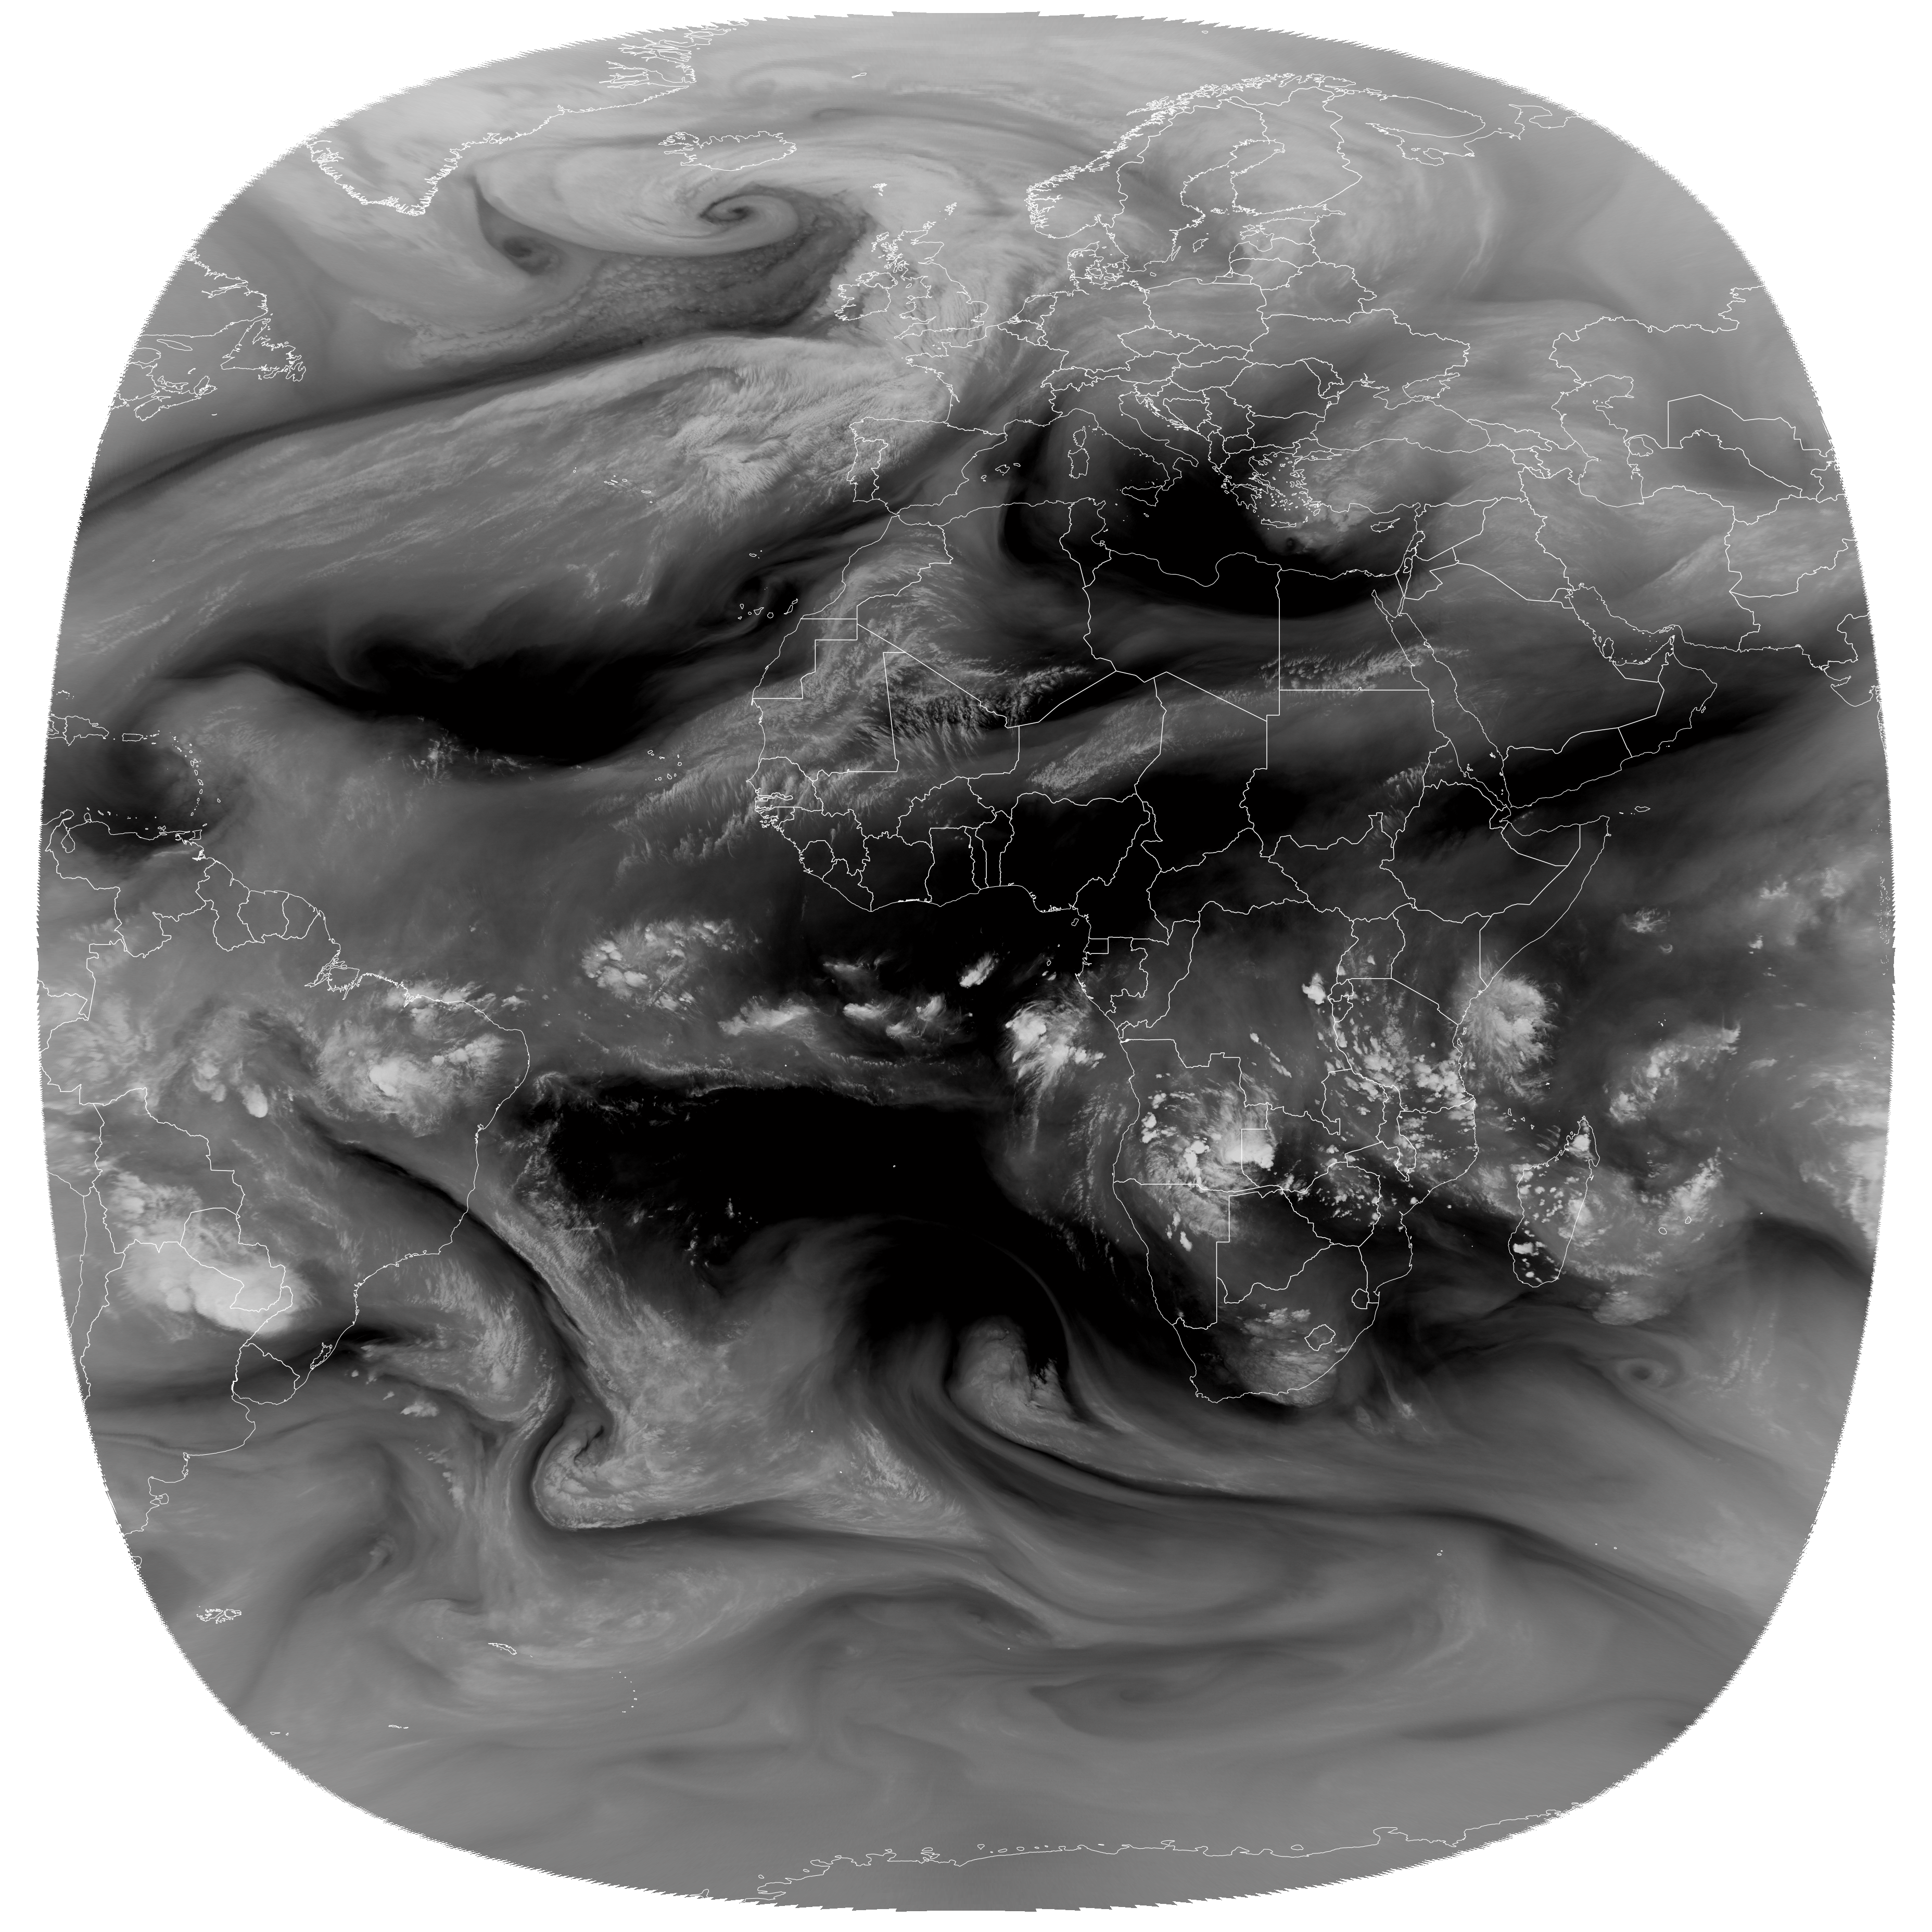
\includegraphics[width=\textwidth]{Chapter2_Theory/images/sat_channels/meteosat-msg_wv062_overlay-ne_10m_coastline_overlay-ne_10m_admin_0_boundary_lines_land.png}
            \caption[Channel WV 6.2]%
            {{\small Channel WV 6.2}}    
            \label{fig:WV_6.2}
        \end{subfigure}
        \hfill
        \begin{subfigure}[b]{0.475\textwidth}  
            \centering 
            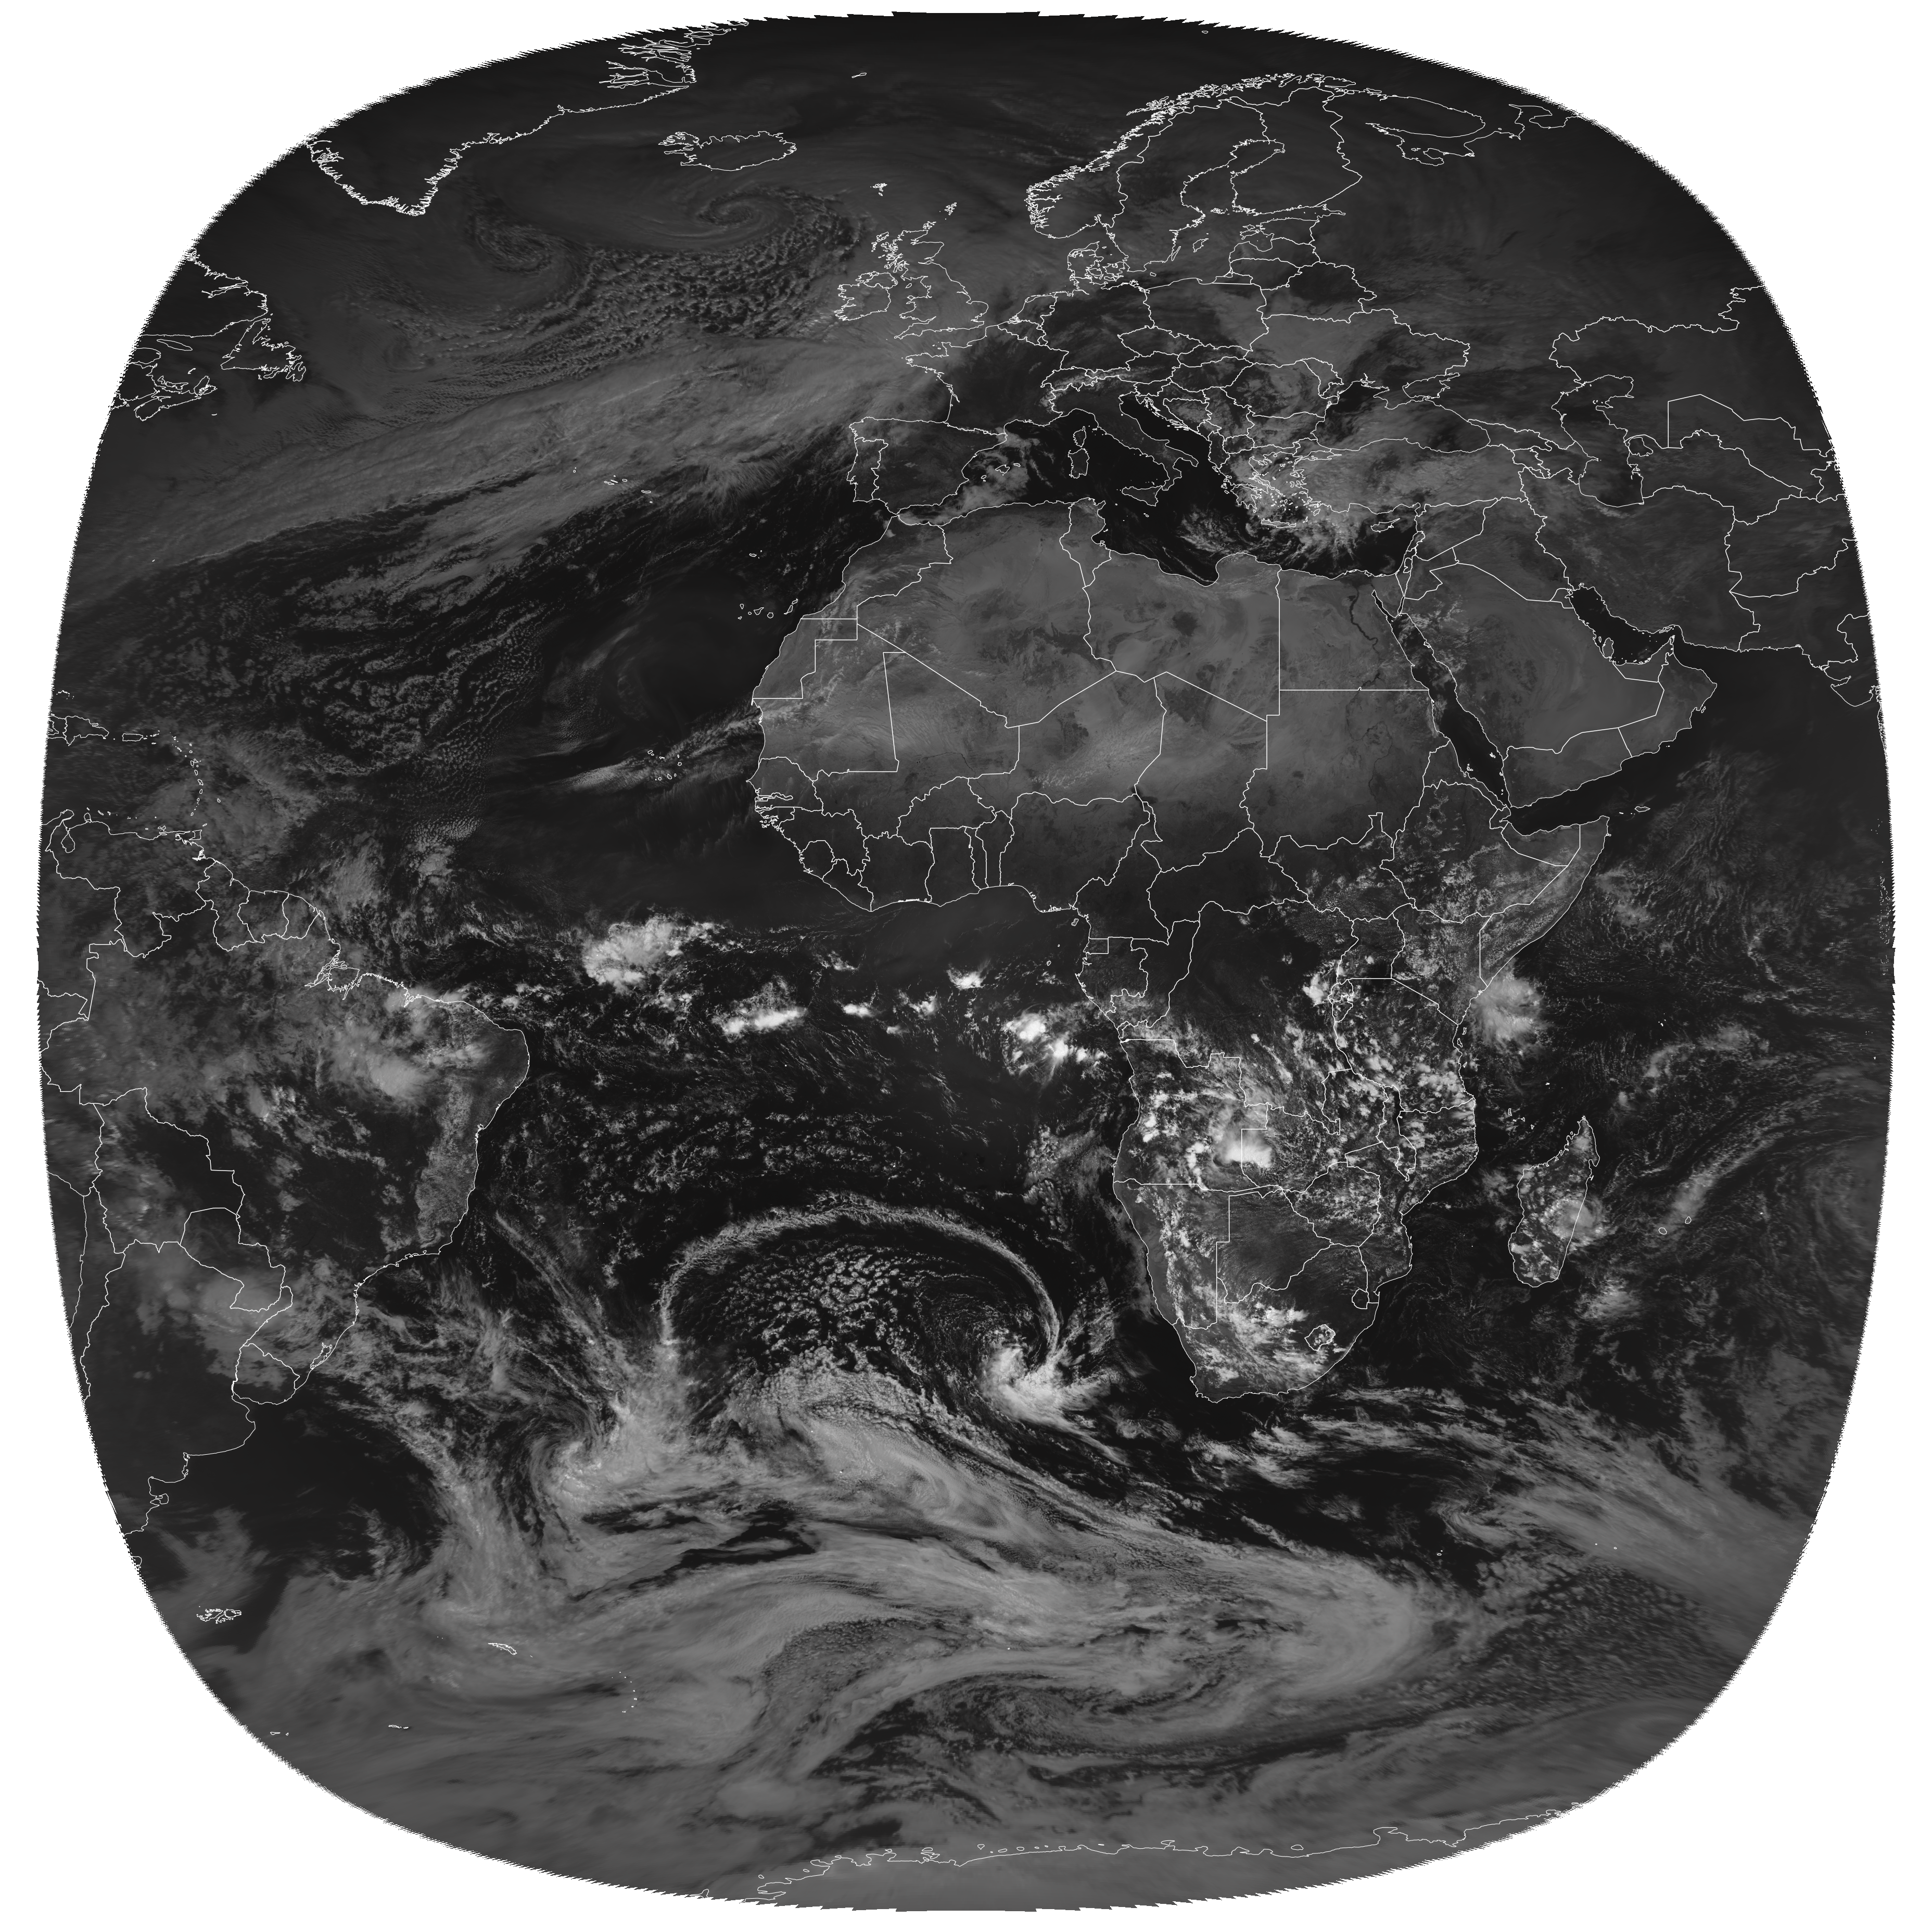
\includegraphics[width=\textwidth]{Chapter2_Theory/images/sat_channels/meteosat-msg_vis006_overlay-ne_10m_coastline_overlay-ne_10m_admin_0_boundary_lines_land.png}
            \caption[]%
            {{\small VIS 0.6}}    
            \label{fig:VIS_0.6}
        \end{subfigure}
        \vskip\baselineskip
        \begin{subfigure}[b]{0.475\textwidth}   
            \centering 
            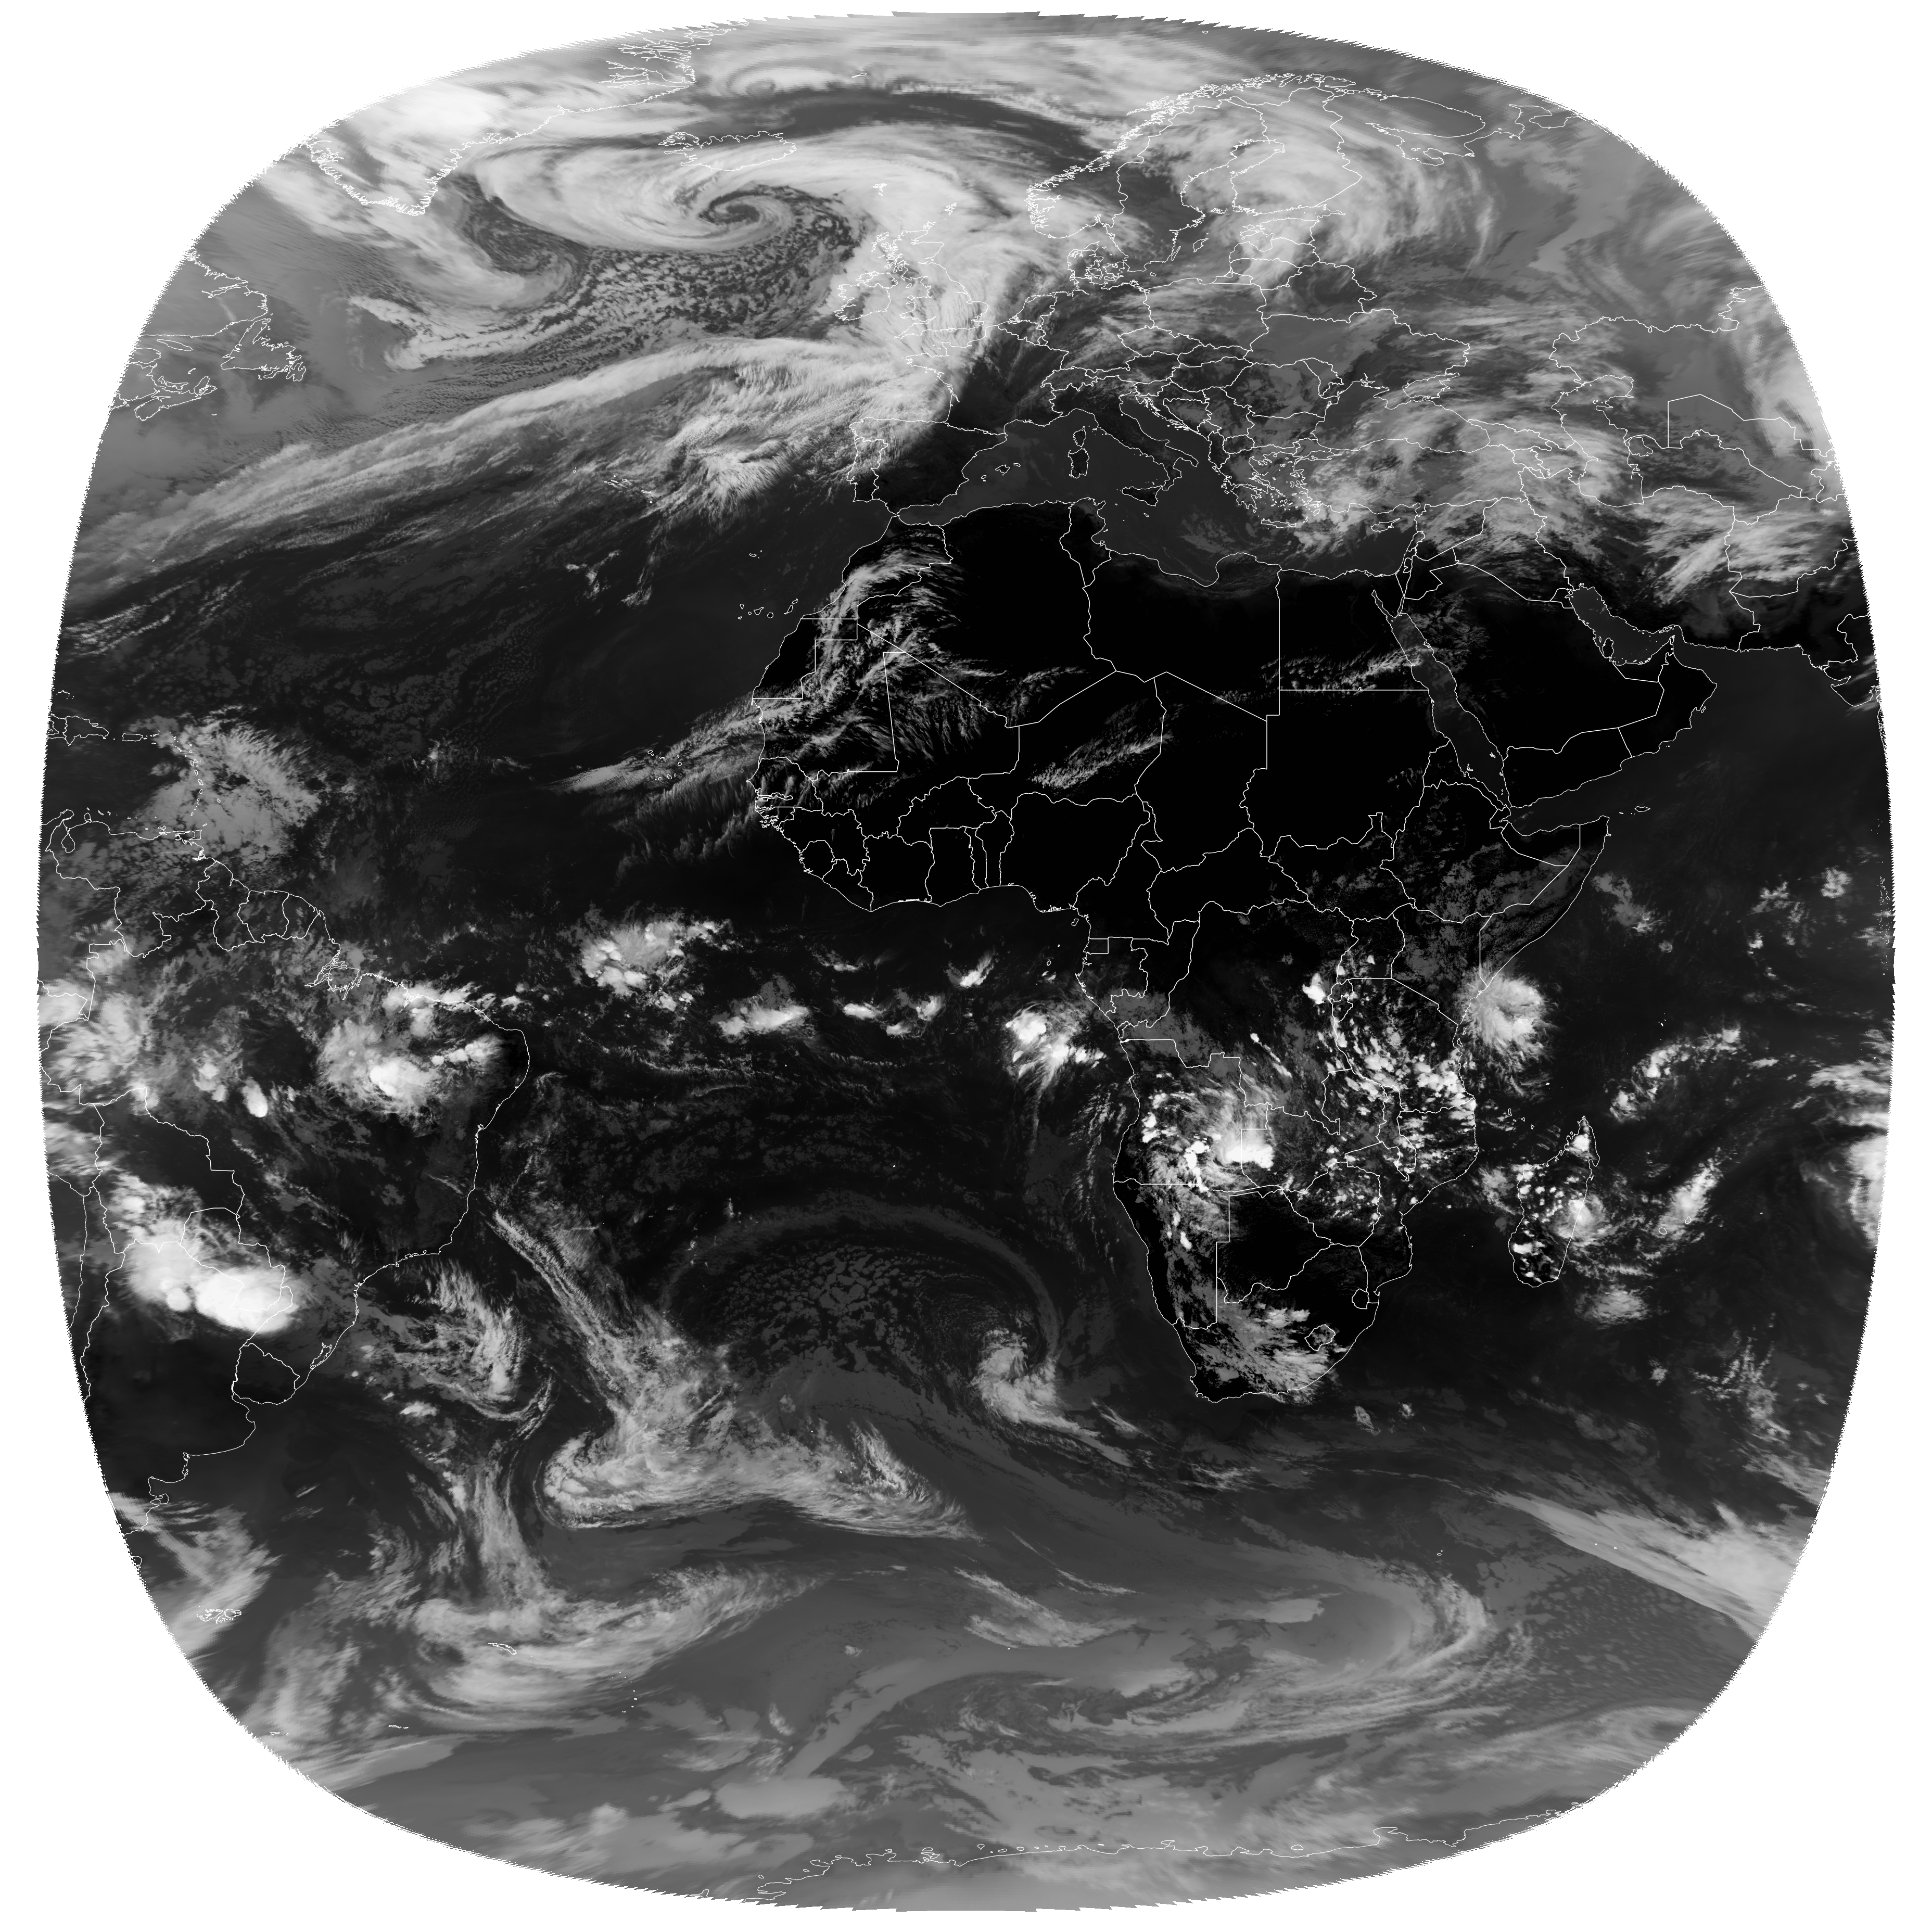
\includegraphics[width=\textwidth]{Chapter2_Theory/images/sat_channels/meteosat-msg_ir108_overlay-ne_10m_coastline_overlay-ne_10m_admin_0_boundary_lines_land.png}
            \caption[something]%
            {{\small IR 10.8}}    
            \label{fig:IR_10.8}
        \end{subfigure}
        \quad
        \begin{subfigure}[b]{0.475\textwidth}   
            \centering 
            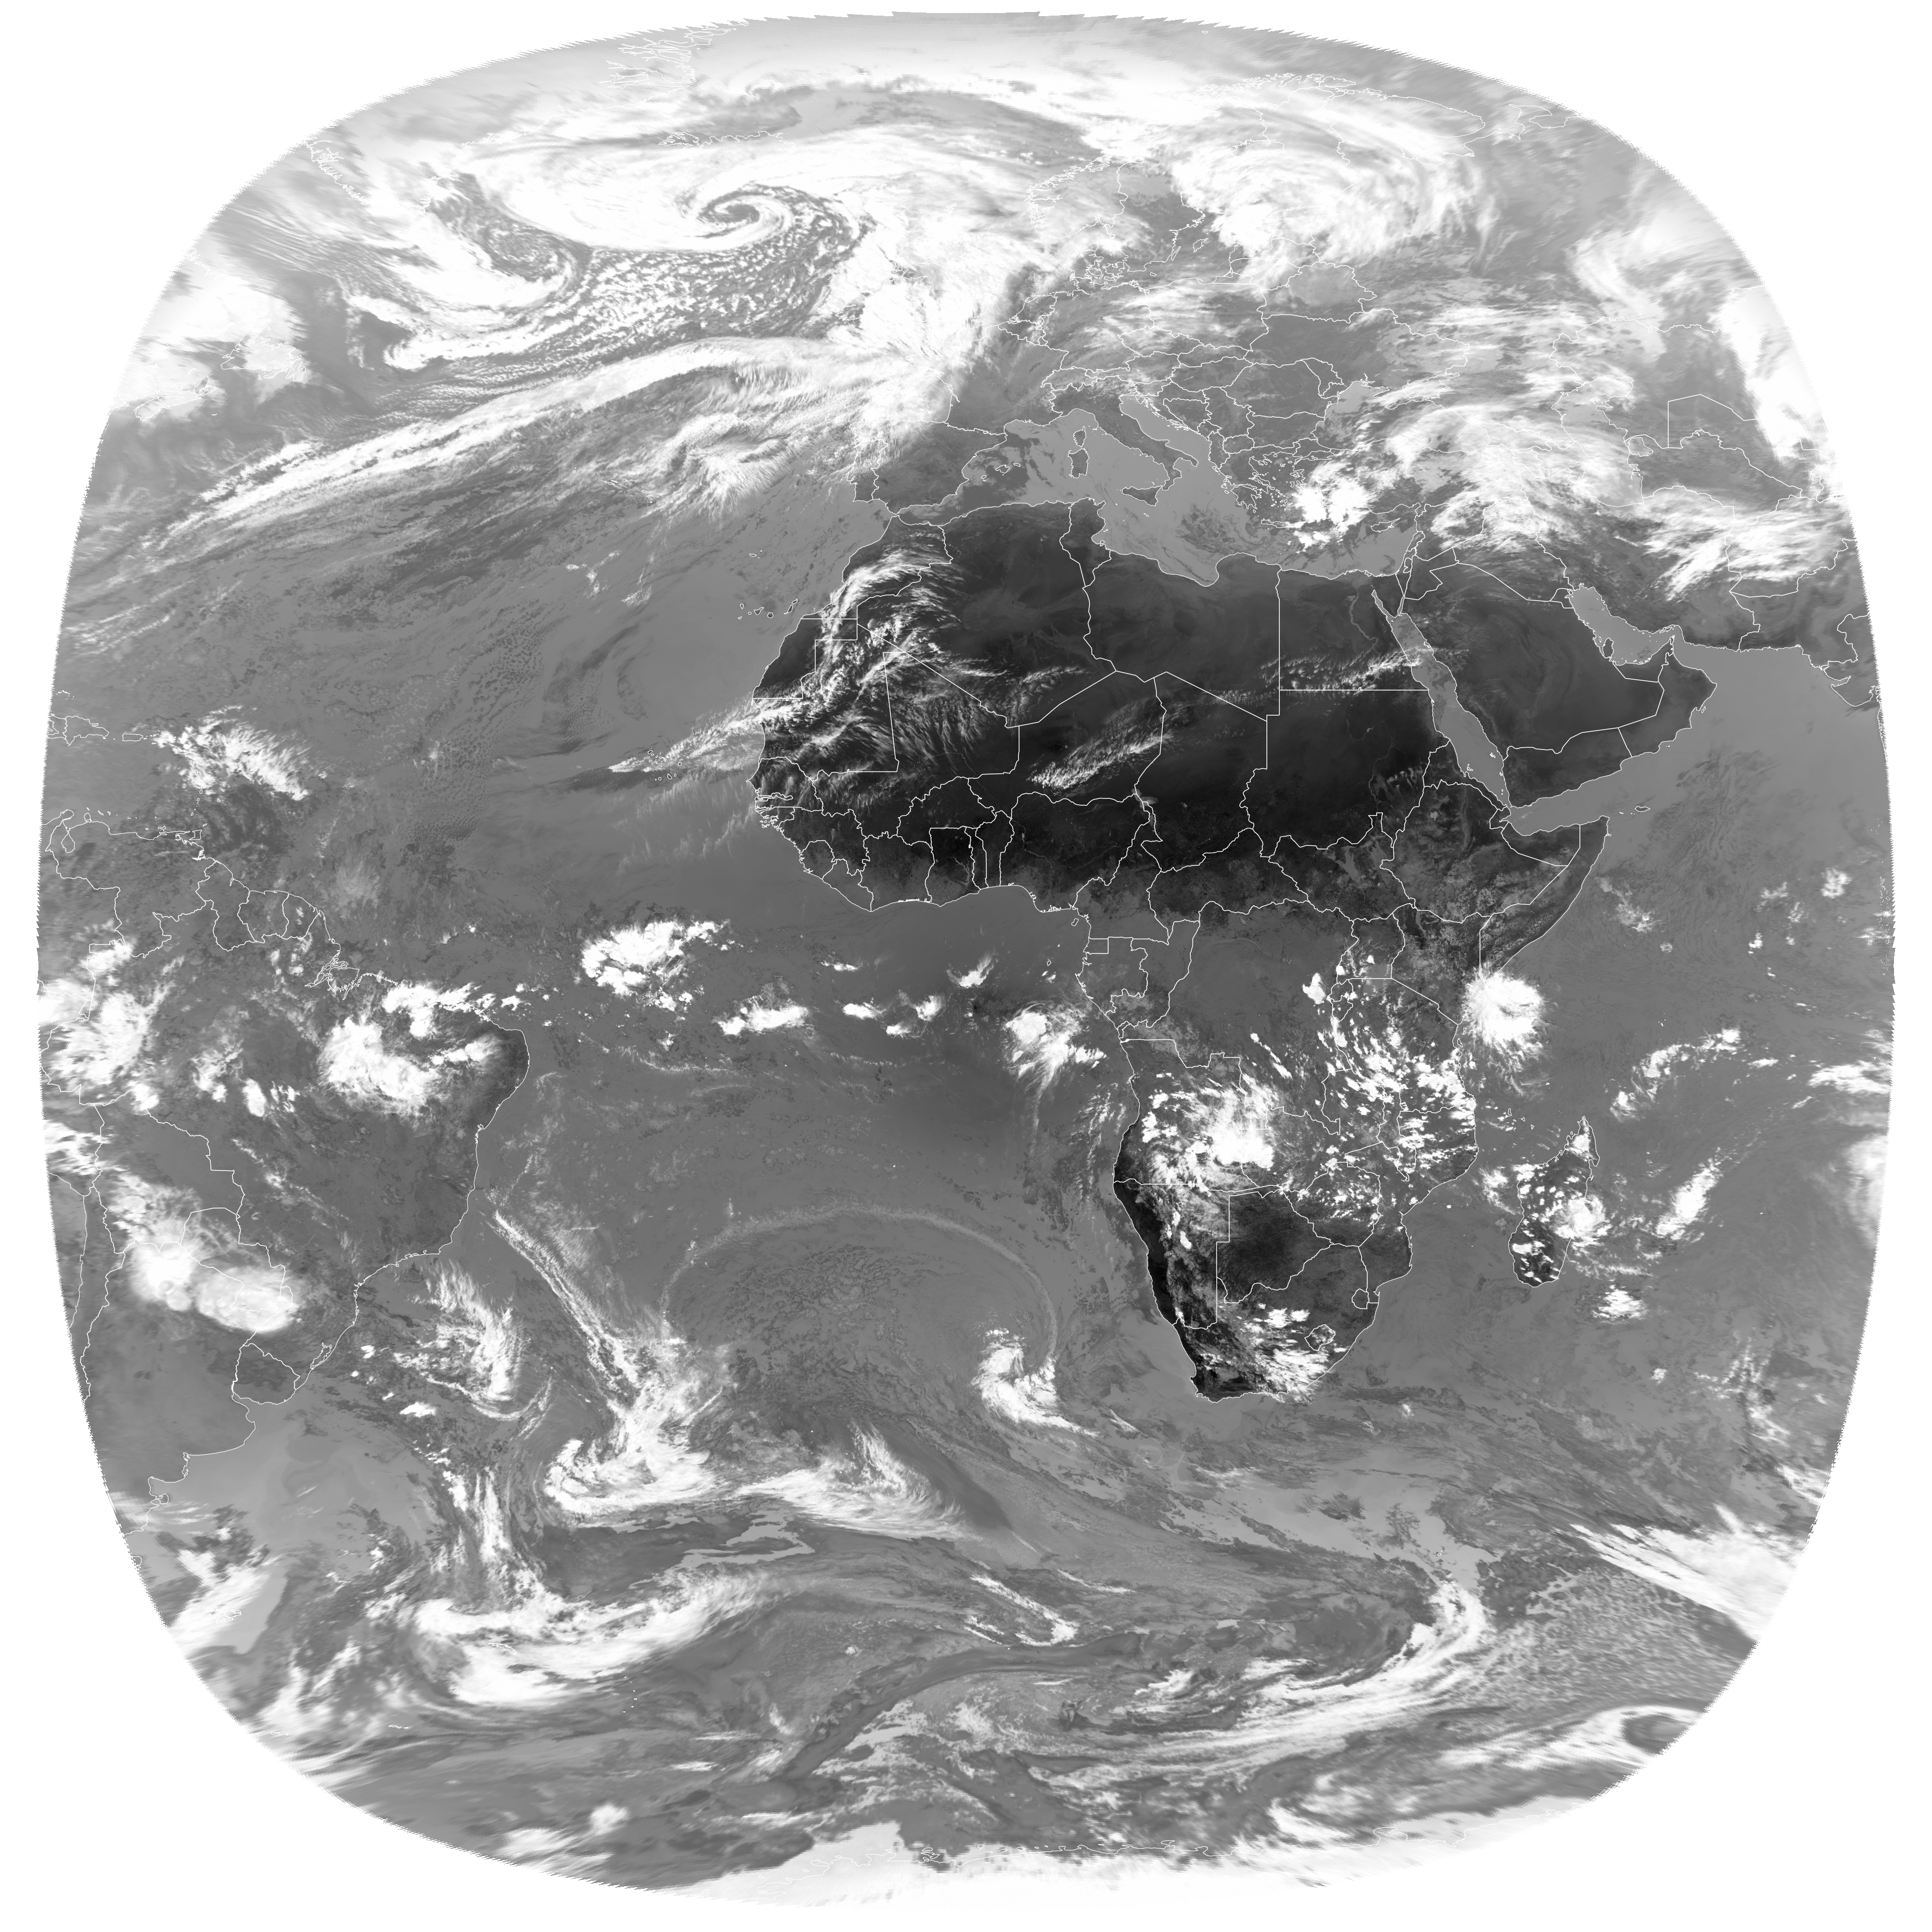
\includegraphics[width=\textwidth]{Chapter2_Theory/images/sat_channels/meteosat-msg_ir039_overlay-ne_10m_coastline_overlay-ne_10m_admin_0_boundary_lines_land.png}
            \caption{{\small IR 3.9}}    
            \label{fig:IR_3.9}
        \end{subfigure}
        \caption{{Spectral bands from SEVIRI. February 15th 2020 at noon. It shows the lowpressure system \textit{Elsa} positioned of the west coast of Iceland. Having a record breaking low of 915hPa (\cite{nrk_lavtrykk}). 
        The images are provided by  \cite{eumetcast_image_gallery}.}
    } 
    \label{fig:SEVIRI_channels}
\end{figure*}

% Info på bildene \textbf{Rectified (level 1.5) Meteosat SEVIRI image data. The data is transmitted as High Rate transmissions in 12 spectral channels. Level 1.5 image data corresponds to the geolocated and radiometrically pre-processed image data, ready for further processing, e.g. the extraction of meteorological products. Any spacecraft specific effects have been removed, and in particular, linearisation and equalisation of the image radiometry has been performed for all SEVIRI channels. The on-board blackbody data has been processed. Both radiometric and geometric quality control information is included. Images are made available with different timeliness according to their latency: quarter-hourly images if latency is more than 3 hours and hourly images if latency is less than 3 hours (for a total of 87 images per day). To enhance the perception for areas which are on the night side of the Earth a different mapping with increased contrast is applied for IR3.9 product. The greyscale mapping is based on the EBBT which allows to map the ranges 200 K to 300 K for the night and 250 K to 330 K for the day.}
% Lastet ned 16.02.2020.
\cite{Karlsson2015AdvancingData} list the five key properties for remote sensing of clouds using passive imagery. To have a reference figure \ref{fig:SEVIRI_channels} shows examples on how different properties are seen by the satellite. This includes the four spectral bands, WV 6.2, VIS 0.6, IR 3.9 and IR 10.8. In general anything that appears bright have a higher reflectance at the \acrfull{toa} than the surface. Lower radiences are displayed in darker colours and brighter is white. Clouds appear bright in VIS and NIR channels, see \ref{fig:VIS_0.6}. Clouds consisting of liquid droplets reflect strongly in SWIR and MWIR. This is shown in figure \ref{fig:IR_3.9}. The earth surface, including snow and ice, appear dark. This allows for detection of low level clouds at night. Exploiting the fact that clouds are not perfectly emitting black bodies. Cloud are typically colder than the earth surface. Cirrus cloud are optically thin, but can be detected using split window channels (IR10.8 and IR12.0) differences. See figure \ref{fig:IR_10.8}. Figure \ref{fig:WV_6.2} shows detected water vapour. In general broken clouds give rise to scattered pattern or texture in images otherwise homogeneous, ice-free ocean for instance. To summaries the success of a screening is dependant on the illumination, the state of the surface and atmosphere (\cite{Karlsson2015AdvancingData}).  The number of spectral bands and footprint size (pixel resolution) determine the practical application a particular retrieval can be used for. Differences in swath width determine the frequency at a given position. Viewing angle affect the optical properties of the medium (but also its apparent position). \textit{Parallax} describes the apparent shift in position of a object, when you move the observer along a axis. This is a issue in remote sensing. Positions of satellites are moved and high viewing angles may cause similar issues. Since the position of objects is relevant to the viewing angle. A high viewing angle may introduce problems with parallax of high clouds. This factor is negligible when detecting low clouds (\cite{Joro2010ComparisonFinland}). Moving the observer (satellite) changes the apparent position of the measurement. 

Differences in sensitivity and retrieval algorithms contribute to a large spread in global mean cloud amount among different cloud products. In their assessment of global cloud datasets \cite{Stubenrauch2013AssessmentPanel} compared the global mean cloud cover of six datasets (ISCCP, PATMOS-x, MODIS-ST, MODIS-CE, AIR-LMD and TOVS Path-B). In this process they eliminating MISR and ATSR-GRAPE because of different observation times (as in Table 3.) and two outlier datasets, HIRS-NOAA and POLDER. Their results show that the difference among the six datasets, the difference is of order 0.08. On the contrary, local differences could be up to 0.4. Its worth noting that the satellite data using in this thesis is not included in  \citeauthor{Stubenrauch2013AssessmentPanel} study, but its illustrates nicely the large differences among other datasets. 

%Cloud-Aerosol Lidar and Infrared Pathfinder Satellite Observations, CALISO is much used in other research because it gives a vertically resolved cloud (3D observations). This additional spatial information is provided on the expense of frequency and uncertainty. \textit{Reason why calipso is ruled out as a candidate. large uncertainty Stubenau} MODIS has low spatial resolution but high temporal resolution, one to two days. National Oceanic and Atmospheric Administration, NOAA \textbf{ something}. Most polar orbiting satellites have a resolution at best daily. \textbf{kilde (shubenau)} \textbf{Does the other one give ferdig produkter av skyfraksjoner og eller er mye lettere og regridde??} The number of channels (higher for other than METEOSAT). The more channels you have the more accurate cloud detection algorihms you can use. Most of the uncertainty in satellite retrivals are attributed to the presence of clouds.  

\textbf{Hugo how much where you thinking of including from other satellites.}

\subsection{METeosat Second Generation, MSG} \label{sec:meteosat}
Prior to the launch of the METeosat researchers discussed the temporal frequency suitable for the observing weather. The METeosat first generation had a temporal resolution of 30min \textbf{kilde}. For the second generation, 15min intervals was chosen to best cope with the short lifetime and rapid deformation of clouds. It was also suggested that a temporal frequency of 1 to 10min is necessary tracking cumulus type clouds. \textbf{kilde stubenau - må være en annen kilde}. This agrees with the table 1.3 in Lohmann et. al. stating the lifetimes of different type clouds. \textbf{kilde Lohmann s. 19} There is a \textit{ring} of geostationary satellites located at equator providing a global covering (not included polar regions). The altitude of satellite determine the forward velocity and is chosen for the geostationary orbit. To achieve this orbit it needs to maintain a height of $\sim 36 000km $. The first Meteosat Second Generation (MSG-1) was lauched 28 August 2002. It became operational 29 January 2004 and got renamed Meteosat-8. The \acrshort{msg} system provides a two satellite system, one operational and one standby. This introduces issues related to the parallax. It becomes evident when comparing simultaneous measurements for the operation and the standby METeosat satellites. \ref{tab:dataset_summary} The operational satellite at a nadir point of $0^o$ latitude. Samples a full disk in cycles of 15min. A full disk is $3712\times 3712$ pixels.
%\textbf{Thoughts:}
%\begin{enumerate}
%    \item Would it be possible to see further north if the altitude where higher? (Wouldn't be geostationary anymore but would you.)
%    \item Må den alltid være på latitude = 0 for å være geostationary? 
%\end{enumerate}
%METeosat is the only geostationary satellite covering the Europe, Africa and India?. Geostationary \textit{ring} of GEO-satellites. 
The \acrfull{msg} was established as a corporation between \acrfull{esa} and \acrfull{eumetsat}. \acrshort{esa} was in charge of developing the prototype of MSG-1. \acrshort{eumetsat} is responsible for maintaining the user requirements, launch procedures, developing ground segments, ensuring over all system consistency and day to day operations.  \acrshort{msg} primary function is to provide a continuous observations of the earths full disk. Near-constant sampling frequency and a geostationary orbit allows for observing weather phenomena occurring on short scales. Since the satellite always is located at $0^o$ the spatial resolution is not constant spatial resolution, unlike the polar orbiting satellites. The resolution becomes coarser with increasing off-nadir viewing angle (\cite{Stubenrauch2013AssessmentPanel}). There are efforts invested in extending the MSG dataset with the MFG, in order to make use of the time series all the way back to 1980. \textbf{kilde, launched 1977} This is requires new cloud detection algorithms since they only have three common channels and two of them are useful for detecting clouds. \textbf{kilde Stöckli} This could potentially be useful in the future. 

On board the \acrshort{msg} is the \acrfull{seviri} imaging radiometer. Its has  12 spectral channels. The scan is done south to north, east to west. The wavelength of the discrete channels are chosen based on heritage from other sensors. One broadband visible channel, three solar channels (0.6, 0.8 and 1.6 $\mu m$) and 8 thermal infrared channels (3.9, 6.2, 7.3, 8.7, 9.7, 10.8, 12.0 and 13.4 $\mu m$) (\cite{Taravat2015MultilayerMasking}). (Taravat, 2015)  This is of great advantage since much of the community already know how to use the \acrshort{seviri} radiance observations. The channels have been chosen based on their ability to detect clouds, water vapour and ozone. More information about what the different channels detect is available in this paper \textit{An introduction to METeosat second generation (MSG)} published in BAMS 2002 (\cite{Schmetz_meteosat_intro}). % \ref{tab:dataset_summary}. 
\begin{figure}[h]
    \centering
    \includegraphics[scale=0.11]{Chapter2_Theory/images/MET10_RGBNatColourEnhncd_FullResolution_20191123120000.jpg}    
    \caption{\textit{Coverage with \acrshort{seviri} on MSG.}The view of the earth from \acrshort{msg}. The picture is dated noon on the 11 November 2019. \textbf{Cite EUMETSAT}. By studying the patterns it becomes evident that clouds are influenced by the circulations. The image is "Natural colors enhanced"}
    \label{fig:sat_view}
\end{figure}
%You may calculate the difference of the measurements, e.g. for channels VIS0.6, IR3.9 and IR10.8 between the two satellites. This will give an estimate how large the measurements differ and as a consequence the products (e.g. cloud mask) will be different.\textbf{also personal correspondance.}
The operational cloud detection algorithm is pixel by pixel. Post processing involves re-classifing isolated pixels. There is a lot of effort invested in new detection algorithms including spatial structures. One of the methods that show potential here is deep learning \textbf{List many sources.}

The viewing angle attributes to small differences in detected cloud mask. Explained by parallax. This becomes evident when the standby and operational satellite scan simultaneously. By default the standby satellite is adjusted to fit the position of the operational. By taking the difference some small patterns becomes visible. This is not accounted/adjusted for when using the data. Sometimes both satellites gather data at the same time. Then the standby-satellite grid is rectified to a a grid of the operational one \textbf{(Personal correspondence EUMETSAT staff).} 

\subsection{EUMETSAT Cloud Mask} \label{sec:EUMETSAT_cloud_mask}

The \acrshort{eumetsat} cloud mask, CLM consist of four classes, described in table \ref{tab:classes_clm}.

\begin{table}[h]
    \centering
    \setlength\extrarowheight{-7pt}
    \begin{tabular}{c|c}
        Class & Description \\ \hline
        0 & Clear sky over ocean \\
        1 & Clear sky over land \\
        2 & Cloudy \\
        3 & No data/ outer space        
    \end{tabular}
    \caption{Description of classes in EUMETSAT Cloud Mask product.}
    \label{tab:classes_clm}
\end{table}
\begin{table}[ht]
    \centering
    \setlength\extrarowheight{-7pt}
    \begin{tabular}{c|c|c}
        Spectral band & Central wavelength $\left( \mu m  \right)$ & Remark \newline 
        (main gaseous observer of window) \\ \hline
        VIS 0.6 & 0.635 & clouds (window)    \\
        VIS 0.8 & 0.81  & clouds (window)     \\
        NIR 1.6 & 1.64  & clouds (window)    \\
        IR 3.9 & 3.92  & clouds  (window)     \\
        WV 6.2 & 6.25 & \acrlong{wv}  \\
        WV 7.3 & 7.35 & \acrlong{wv}  \\ 
        IR 8.7 & 8.7 &   clouds  (window)       \\
        IR 9.7 & 9.66 & Ozone        \\
        IR 10.8 & 10.8 & Cirrus Clouds (window)  \\
        IR 12.0 & 12 & Cirrus Clouds (window) \\
        IR 13.4 & 13.4 & Carbon Dioxide  \\
        HRV & 0.75 & \acrlong{wv}/ window 
    \end{tabular}
    \caption{Summary of spectral bands, central wavelength and their respective retrieval abilities (\cite{Schmetz_meteosat_intro}). \textbf{Double check remark column wft is a window}}
    \label{tab:msg_spectral_bands}
\end{table}

These classes are derived from almost all channels except HRV and isolated pixels are reclassified \textbf{cite article 10 in Tavarat, 2015}. The cloud mask is distributed in GRIdded Binary or General Regularly-distributed Information in Binary form (GRIB) (no coordinates) and network Common Data Form (NetCDF) (coordinates). The data is available on Earth Observation Portal on EUMETSATS web pages. 

%\begin{figure}[h]
%    \centering
%    \includegraphics[scale = 0.6]{Chapter2_Theory/images/coordinates.png}
%    \caption{Credit, https://tex.stackexchange.com/questions/159445/draw-in-cylindrical-and-spherical-coordinates}
%    \label{fig:coords}
%\end{figure}
%The cloud cover will be referred to as cloud amount, fraction or simply the clouds.
%%%%%%%%%%%%%%%%%%%%%%%%%%%%%%%%%%%%%%%%%%%%%%%%%%%%%%%%%%%%%

\section{Practical implications - OUTDATED} \label{sec:practical_implications}
It is necessary to have a understanding of the needs of the end product before conducting large machine learning projects. Answering questions like: What will it be used for and how can it be implemented in useful way?

A major downside of the data driven learning approach is the rigid resolution. A trained model can only be used on similar problems, with the same spatiotemporal resolution. For applications like climate models, output comes in a wide range of different resolutions. Before implementing the finished product in a new model of a different resolution, it would need to be retrained on the resolution of the climate model under development. This process involves both remapping of the dataset and retraining the model at the correct resolution. This is a time consuming process involving finding a new set of hyperparameters suitable for the new resolution. % It essentially means starting over.

Once trained on global climate datasets, machine learning models provide fast results even for complex parameterisation which is what makes them suitable for the application of climate modelling. Most machine learning packages are developed using Python. \acrfull{esm} are implemented in python. Methods for including the trained parameterizations need to be developed.
 
\subsection{Any implications based on the results presented in this chapter.}

\subsubsection{summary}
This thesis aim to devolop and/or explore methods of parameterising cloud cover based on macro-scale variables like humidity, surface temperature and pressure. Regressing historical observations against macro physical properties which affect clouds. Moving away from the subgrid scale processes. Wish to answar weather there be enough information in humidity, temperature and surface pressure to predict clouds in a time and space.



% Kommentarer fra Hugo om skriving : Teoridelem om satelitter hva er nevn flere og deres oppløsning og hva er fordelen og ulemepen med dem. 
%  Legg inn helt generelle ting i teoretical background åså diskuter selve datasettet i metoden.

% Ignorer artifakten men kommenter i resultatene, keep in mind the artifact is present. 
% Fixed input length, normally one would add 0 if it not present. We need to find a value to add. 
% Scaling is smart due to numerical error not necessarily a requirement for the statistical models. 
% Missing values can be dealt with in two ways. 
% 1) Calculate the average ()
% 2) Predict the missing values - as always this might lead to a unnatural smoothness. 
% 3) 
\cleardoublepage

%\setcounter{chapter}{2}
\chapter{Numerical Methods} \label{ch:num_methods}

In this section we introduce the computational methods used for generating the numerical experiments conducted in this thesis, starting with a short introduction to artificial intelligence. We will give a brief introduction to the biological mechanisms the algorithms in this thesis draw inspiration from. This helps to gain insight to possible applications of different structures. 
%Presenting the autoregressive model and convolutional long short-term memory. The performance metrics used to evaluate their performance and finishing of with automatic optimization routines.
% based on bio-inspired mechanisms are introduced
The task of forecasting in time and space requires two types of intelligence. One is computer vision, to understand the spatial relation and use the underlying physical properties. The other is sequential modelling to understand the temporal evolution.

Two approaches will be explored: autoregressive models (AR) and Convolutional Long Short-Term Memory Network (ConvLSTM). The AR model describes a time varying process, depending linearly on it previous values. The ConvLSTM is used to find a non-linear relation that describes phenomena varying in both time and space. %Another method used is the ConvLSTM.
The aim of this study is to determine whether the concatenation of linear models, or the more advanced non-linear model are better at prediction the complex phenomena varying in time and space.
%When used in tandem (all the linear models?), these models can predict complex natural phenomena ++++ .
The popularity of DL can be partly explained by its flexibility. This flexibility allows deep learning to be applied across many domains. The algorithms discussed here are simply a mathematical framework for learning model representations in data. The process of training is repeated until the network reaches an acceptable performance. In other words \textit{the extent to which this potential can be exploited is limited to the effectiveness of the training procedure applied} and also the data its provided. 

\section{Artificial intelligence}
\begin{figure}[h] % h means place here if possible
    \centering
    \begin{tikzpicture}
        \draw [black, fill=orange, opacity = 0.3]  (2, -0.65) ellipse (2.5 and 1.25); % DL 
        \draw [black, fill=orange, opacity = 0.3]  (2, -0.25) ellipse (4 and 2); % ML
        \draw [black, fill=orange, opacity = 0.3]  (2, 0) ellipse (5.5 and 2.75);     % AI
        \node at ($(2, 2.125)$) {\Large Artificial Intelligence}; % +(2 and -0.65)
        \node at ($(2, 0.9)$) {\Large Machine Learning};
        \node at ($(2, -0.65)$) {\Large Deep Learning};
    \end{tikzpicture}
    \caption{Graph illustrating the subfields of \acrshort{ai}. \acrshort{ml} is a subfield of \acrshort{ai}, \acrshort{dl} is again a subfield of \acrshort{ml}. The sketch is inspired by Figure 1.1 in \citeauthor{chollet_book} (\citeyear{chollet_book}, p.5).}
    \label{fig:subcategories_AI}
\end{figure}
%\begin{figure}[h] % h means place here if possible
    \centering
    \begin{tikzpicture}
        \draw [black, fill=orange, opacity = 0.3]  (2, -0.65) ellipse (2.5 and 1.25); % DL 
        \draw [black, fill=orange, opacity = 0.3]  (2, -0.25) ellipse (4 and 2); % ML
        \draw [black, fill=orange, opacity = 0.3]  (2, 0) ellipse (5.5 and 2.75);     % AI
        \node at ($(2, 2.125)$) {\Large Artificial Intelligence}; % +(2 and -0.65)
        \node at ($(2, 0.9)$) {\Large Machine Learning};
        \node at ($(2, -0.65)$) {\Large Deep Learning};
    \end{tikzpicture}
    \caption{Graph illustrating the subfields of \acrshort{ai}. \acrshort{ml} is a subfield of \acrshort{ai}, \acrshort{dl} is again a subfield of \acrshort{ml}. The sketch is inspired by Figure 1.1 in \citeauthor{chollet_book} (\citeyear{chollet_book}, p.5).}
    \label{fig:subcategories_AI}
\end{figure}
In encounters with geoscientists the author often get the question: \textit{What is the difference between machine learning and artificial intelligence?} They are not different fields, but machine learning (ML) is a subfield of AI. In fact, it is worth mentioning that there is a subfield of ML known as deep learning (DL) (see graph in Figure \ref{fig:subcategories_AI}). DL is at the frontier of AI, with many recent advances being made in this subfield. %Deep learning is a subfield of machine learning, making it a subfield of artificial intelligence. %Deep learning provide a improved. 
The origin of the subfields has a historical explanation. Each subfield is linked to significant advances, which will be explained using parallels to the long standing problem of computer chess. 
\begin{figure}[h] % h means place here if possible
\centering
\def\layersep{2.5cm}
\begin{tikzpicture}[shorten >=1pt,->,draw=blue, node distance=\layersep]
    \tikzstyle{every pin edge}=[<-,shorten <=1pt]
    \tikzstyle{neuron}=[circle,fill=black!25,minimum size=17pt,inner sep=0pt]
    \tikzstyle{input neuron}=[neuron, fill=green];
    \tikzstyle{output neuron}=[neuron, fill=red];
    \tikzstyle{hidden neuron}=[neuron, fill=cyan];
    \tikzstyle{annot} = [text width=4em, text centered]

    \node[input neuron] (I-1) at (0,-1) {}; % {$T_{2m}$};
    \node[input neuron] (I-2) at (0,-2) {}; % {$q_v$};
    \node[input neuron] (I-3) at (0,-3) {}; % {$RH$};
    \node[input neuron] (I-4) at (0,-4) {}; % {$p_s$};

    % Draw the input layer nodes
    %\foreach \name / \y in {1,...,4}
    % This is the same as writing \foreach \name / \y in {1/1,2/2,3/3,4/4}
    %    \node[input neuron, pin=left:Input \#\y] (I-\name) at (0,-\y) {};

    % Draw the hidden layer nodes
    \foreach \name / \y in {1,...,5}
        \path[yshift=0.5cm]
            node[hidden neuron] (H-\name) at (\layersep,-\y cm) {};

    % Draw the output layer node
    \node[output neuron, right of=H-2] (O) {};
    \node[output neuron, right of=H-3] (O1) {};
    \node[output neuron, right of=H-4] (O2) {};


    % Connect every node in the input layer with every node in the
    % hidden layer.
    \foreach \source in {1,...,4}
        \foreach \dest in {1,...,5}
            \path (I-\source) edge (H-\dest);

    % Connect every node in the hidden layer with the output layer
    \foreach \source in {1,...,5}
        \path (H-\source) edge (O);
        %\path (H-\source) edge (o1);
        %\path (H-\source) edge (o2);

    % Does the same thing the loop does had to do it manually tho
    \path (H-1) edge (O1);
    \path (H-2) edge (O1);
    \path (H-3) edge (O1);
    \path (H-4) edge (O1);
    \path (H-5) edge (O1);
    
    \path (H-1) edge (O2);
    \path (H-2) edge (O2);
    \path (H-3) edge (O2);
    \path (H-4) edge (O2);
    \path (H-5) edge (O2);

    % Annotate the layers
    \node[annot,above of=H-1, node distance=1cm] (hl) {Hidden layer};
    \node[annot,left of=hl] {Input layer};
    \node[annot,right of=hl] {Output layer};
\end{tikzpicture}
\caption{Fully connected feed forward neural network with one hidden layer. The connections between the layers are the weights. The sketch is based on the example \citepaper{ffnn}.}
\label{fig:one_layer_mlp}
\end{figure}
%The input layer has four units, the hidden layer has five and the output layer has three. In total there are 35 parameters in this network (37 if bias is included).
Figure \ref{fig:one_layer_mlp} illustrates a simple artificial neural network. Artificial intelligence (AI) in general and Deep Learning (DL) in particular emerged from biological inspired computing. Many of the DL network architectures draw inspiration from the human brain. The architecture of DL, while distinct from biological computing, is named such that concepts in neuroscience and computing can be treated analogously. For example using building blocks such as neurons (nodes, units), weights (connections between neurons), rules of signal propagation, activation (transfer function) and learning algorithms (training algorithms). % \textbf{Raymond: Må skille mellom AI og DL - AI er ikke nødvendigvis basert på en modell av hjernen.}

The circles illustrate nodes (neurons). Nodes belonging to the same layer is shown in one color. Arrows illustrates weights, the connections between the layers. Nodes belonging to the same layer are not connected, but nodes in consecutive layers are connected with weights. 
% \textbf{cite \href{https://www.sciencedirect.com/topics/engineering/neural-network-architecture}{\textbf{https://www.sciencedirect.com/topics/engineering/neural-network-architecture}}}

% For mye om receptive field.
Sequence modelling draws parallels to the human memory. This type of modelling requires information about earlier stages, this is stored in memory. 
%Image recognition and sequence modelling draw parallels to human vision and memory, respectively. 
Simple models have one memory centre. Drawing inspiration from the brain, other more complex models make the distinction between a short term and a long memory centre. Finishing sentences for others is a trivial task for humans. The reader should not be surprised that by the following \textit{the clouds are in the \ldots sky} \cite{colah_blog_post}.


Three factors determine advances in the field of AI: data, hardware, and algorithms \cite{chollet_book}. This explains why there often is a significant time gap between an idea and breakthroughs in the architectures and results. CNNs, for example, were conceptually developed in the 80s, but a lack of sufficient computing power (hardware) kept their use in hibernation until 2012, when a CNN (AlexNet) won the ImageNet challenge, an image recognition contest \textbf{(Citation)}.

AI started by automating tasks normally performed by humans. Computer chess is the longest studied problem in the history of artificial intelligence and advancements in computer chess provide good examples on the evolution of AI. In 1951, Alan Turing was the first to publish a program, on paper, capable of playing a entire game of chess. 
% In media (and other places) the terms AI and ML are often used together. This can be considered
% The terms are often used interchangeably or together like \textit{AI and ML}, this can be confusing for someone not in this field.
\textbf{Første model for ANN (Artificial Neural Network) ble laget i 1943. ``Perceptron'' ble beskrevet i 1958, første multi-layer network publisert i 1965, ``continuous backpropagation'' ble utledet i 1960/1961, \ldots ANN/DL har altså en lang historie, i hovedsak drevet av forbedrede algoritmer, men det er først det siste tiåret at maskinvaren er blitt kraftig nok til at neuralnettverk, og da i første rekke ved hjelp av grafikkakseleratorer (GPU).}

Because this program used explicitly trained programs rather than developing its own "knowledge" from supplied examples, this falls into the category of ML and not the base category of AI. ML is distinct in that it attempts to deduce rules and go beyond human intuition using a complex net of interactions. 
\textbf{Turing's sjakkprogram er vel strengt tatt heller et eksempel på ``Rule-Based AI''? Alle reglene var bestemt på forhånd, men programmet prøvde for hvert trekk å finne det beste alternativet ut fra tilstanden på brettet og hvilke muligheter motspilleren ville få i sitt neste trekk.}
% (leads into architecture paragraph)

%Starting with explicitly trained programs. This falls in the category of AI and not ML.
%\textit{Learning, in the context of ML, describes the automatic search for a better representations.} 
%The network is presented with many examples and is trained, rather than explicitly programmed. 
Geoscientists may be more familiar with the concept of "calibration" when it comes to statistical models, which essentially is the same process. In the context of deep learning, ``deep'' refers to the number of layers contributing to a network, and thus the complexity of relationship between input variables. DL expands the ideas from ML using deeper networks, \textit{i.e,} more layers.
%\textbf{``e.g.'' betyr ``exempli gratia'', altså for eksempel; ``i.e.'' betyr ``id est'' -- ``det er'', ``altså''}
\textbf{Er ``backpropagation'' også en av forskjellene mellom ML og DL? Jeg er uklar om ``backpropagation'' brukes i ML utenfor DL.}

%Geoscientists may be more familiar with the concept of "calibration" when it comes to statistical models, which essentially is the same process. In the context of deep learning, deep references to the number of layers contributing to a network, and thus the complexity of relationship between input variables. DL expands the ideas from ML using deeper network, e.g. more layers. 
\begin{figure}[h] % h means place here if possible
\centering
\def\layersep{2.5cm}
\begin{tikzpicture}[shorten >=1pt,->,draw=blue, node distance=\layersep]
    \tikzstyle{every pin edge}=[<-,shorten <=1pt]
    \tikzstyle{neuron}=[circle,fill=black!25,minimum size=17pt,inner sep=0pt]
    \tikzstyle{input neuron}=[neuron, fill=green];
    \tikzstyle{output neuron}=[neuron, fill=red];
    \tikzstyle{hidden neuron}=[neuron, fill=cyan];
    \tikzstyle{annot} = [text width=4em, text centered];

    % Determining the input layer.
    \node[input neuron] (I-1) at (0,-1) {}; % {$T_{2m}$};
    \node[input neuron] (I-2) at (0,-2) {}; % {$q_v$};
    \node[input neuron] (I-3) at (0,-3) {}; % {$RH$};
    \node[input neuron] (I-4) at (0,-4) {}; % {$p_s$};

    % Draw the input layer nodes
    %\foreach \name / \y in {1,...,4}
    % This is the same as writing \foreach \name / \y in {1/1,2/2,3/3,4/4}
    %    \node[input neuron, pin=left:Input \#\y] (I-\name) at (0,-\y) {};

    % Draw the hidden layer nodes
    \foreach \name / \y in {1,...,5}
        \path[yshift=0.5cm]
            node[hidden neuron] (H-\name) at (\layersep,-\y cm) {};

    % Connect every node in the input layer with every node in the
    % hidden layer.
    \foreach \source in {1,...,4}
        \foreach \dest in {1,...,5}
            \path (I-\source) edge (H-\dest);

    % Draw the hidden layer nodes
    \foreach \name / \y in {1,...,5}
        \path[yshift=0.5cm]
            node[hidden neuron] (R-\name) at (2*\layersep,-\y cm) {};

    % Connect every node in the input layer with every node in the
    % hidden layer.
    \foreach \source in {1,...,5}
        \foreach \dest in {1,...,5}
            \path (H-\source) edge (R-\dest);

    % Draw the hidden layer nodes
    %\foreach \name / \y in {1,...,5}
    %    \path[yshift=0.5cm]
    %        node[hidden neuron] (T-\name) at (3*\layersep,-\y cm) {};

    % Draw the hidden layer nodes
    \foreach \name / \y in {1,...,5}
        \path[yshift=0.5cm]
            node[hidden neuron] (L-\name) at (4*\layersep,-\y cm) {};

    % Connect every node in the input layer with every node in the
    % hidden layer.
    \foreach \source in {1,...,5}
        \foreach \dest in {1,...,5}
            \path[dashed] (R-\source) edge (L-\dest);



    % Connect every node in the input layer with every node in the
    % hidden layer.
    %\foreach \source in {1,...,5}
    %    \foreach \dest in {1,...,5}
    %        \path (R-\source) edge (T-\dest);



    % Draw the output layer node
    \node[output neuron, right of=L-2] (o1) {};
    \node[output neuron, right of=L-3] (o2) {};
    \node[output neuron, right of=L-4] (o3) {};

    % Connect every node in the hidden layer with the output layer
    \foreach \source in {1,...,5}
        \foreach \dest in {1,...,3}
            \path (L-\source) edge (o\dest);

    % Annotate the layers
    \node[annot,above of=H-1, node distance=1cm] (hl) {Hidden layer};
    \node[annot,above of=R-1, node distance=1cm] (hr) {Hidden layer};
    %\node[annot,above of=T-1, node distance=1cm] (ht) {Hidden layer};
    \node[annot,above of=L-1, node distance=1cm] (hL) {Hidden layer};

    \node[annot,left of=hl] {Input layer};
    \node[annot,right of=hL] {Output layer};
\end{tikzpicture}

\caption{Deep fully connected neural network. The sketch is based on the example \cite{ffnn}.}
\label{fig:multilayer_mlp}
\end{figure}
Figure \ref{fig:multilayer_mlp} illustrates a deeper version of the network displayed in Figure \ref{fig:one_layer_mlp}. A layer is a set of nodes. The connections between the layers are the trained units, also known as weights. To distinguish from deep learning, traditional machine learning is sometimes referred to as shallow learning. Linear regression (LR) is ML algorithm predating computers which is still useful today. Traditional LR can be derived using shallow learning methods. 

Intelligence, in the context of artificial intelligence, is still a topic of debate. Traditionally, a machine would be considered intelligent if it could beat a human at a given task. For computer chess, this was achieved in 1997 when IBM's DeepBlue beat Gary Karsparov. Researchers had learned how to build a chess-playing AI, but not a program that could generalize to anything beyond similar boardgames. \textbf{Raymond: DeepBlue var i hovedsak regel-basert, men Google's AlphaZero er (delvis) basert på DL.}

In retrospect, scientist have realized that this particular architecture is not be informative on human intelligence. See the paper from to get more information about the specifics \textbf{cite paper}. Based on psychology studies it is clear that the game of chess involves complex reasoning, search, perceptual and memorial processes. While one can solve chess using these abilities, one can also solve chess by taking radical shortcuts, that the human mind is not capable of. 
 

% Explain glossaries or words that are used a lot.
%Intelligence, in the context of artificial intelligence, is still a topic of debate. Traditionally, a machine would be considered intelligent if it would beat a human at a given task. For computer chess, this was achieved in 1997 when IBM's DeepBlue beat Gary Karsparov. Researchers had learned how to build a chess-playing AI, but not a program that could generalize to anything beyond similar boardgames. In retrospect, scientist have realized that this particular architecture is not be informative on human intelligence. See the paper from to get more information about the specifics \textbf{cite paper}. Based phsycology studies its clear that the game of chess involves complex reasoning, search, perceptual and memorial processes. While one can solve chess using these abilities, one can also solve chess by taking radical shortcuts, the human mind is not capable of. 
%Researchers became aware that they had learned less to nothing about how the human mind works. The original understanding of machine intelligence has been abandoned in search for a more complete definition. \textbf{chollet google artikkel}

There are several different types of machine learning, each suitable for solving different tasks. Figure \ref{fig:machine_learning_categories} shows the types of ML and their subcategories. These subcategories also exist for deep learning, the only difference being the number of layers used.
%, but in order to keep this as general they are described from the above level. Keep in mind that their deep learning cousins can be referred to by simply adding the prefix 'deep'. 
% Example on deep reinforcement learning.
%The frontier of chess playing programs is AlphaZero. The deep reinforcement learning architecture trained is using self-play. Without having any previous knowledge of rules. 

%Supervised learning is the part of machine learning concerned with learning the relation between input data, x and labelled data, y. Regression predict continuous values. Replicating a function. Classification is discrete, since it assigns a category to the input. 
%Reinforcement learning is a goal-oriented algorithms, most known for playing chess, solving labyrinths and lately \textcolor{red}{for?} active flow control \textbf{Cite Jean Rau, three papers}. \textcolor{red}{(Nytt avsnitt?)} 
%Unsupervised learning tries to detect patterns in unlabelled data. This includes clustering and dimensionality reduction. Dimensionality reduction has been used by climatologist for decades in order to remove seasonal variation \textbf{cite Benestad}. Unsupervised and reinforcement learning is out of the scope of this thesis and will not be discussed further.
%author : Hanna Svennevik
\begin{figure}[h] % h means place here if possible
    \centering
    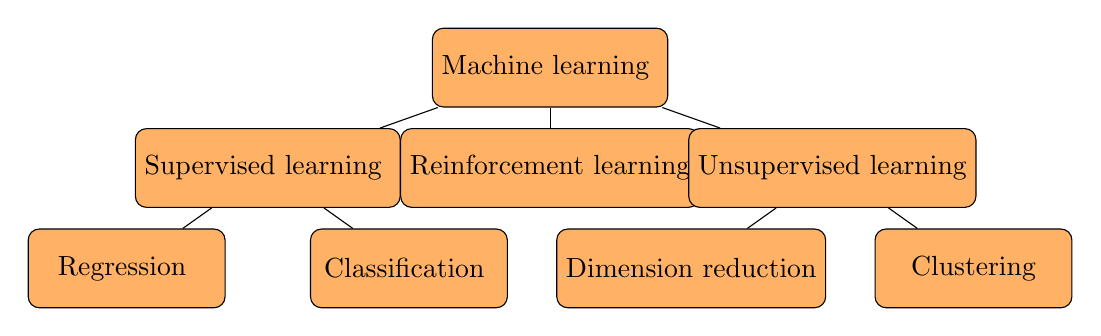
\begin{tikzpicture}[sibling distance=12em,scale = 0.85,
  every node/.style = {shape=rectangle, rounded corners,
    draw, align=center, 
    %top color=white, bottom color=cyan!20,
    fill=orange!60, minimum width=2.5cm, minimum height = 1.0cm}]]
  \node { Machine learning }
    child { node {  Supervised learning  } 
        child { node {  Regression   } }
        child { node {  Classification  } }
    }
    child {node {Reinforcement  learning}}
    child {node {Unsupervised learning}
           child { node {Dimension reduction}}
           child { node {Clustering}}};
\end{tikzpicture}
    \caption{The graph shows the different type of machine learning and their subcategories.}
    \label{fig:machine_learning_categories}
\end{figure} 

\begin{itemize}
    \item \textbf{Supervised learning}: part of machine learning concerned with learning the relation between input data, x and labelled data, y.
    \begin{itemize}
        \item Regression\\predict continuous values. Replicating a function.
        \item Classification\\discrete, since it assigns a category to the input.
    \end{itemize}
    \item \textbf{Unsupervised learning}: Detecting patterns in unlabeled data.
    \begin{itemize}
        \item Clustering\\Grouping a set of data points into a predescribed number of groups
        \item Dimension reduction\\Reducing the number of random variables under consideration.
    \end{itemize}
    \item \textbf{Reinforcement learning}: Goal oriented algorithms.
\end{itemize}

\subsection{Autoregressive models} \label{sec:ARmodels}
The autoregressive model (AR) is a form of linear model where values from previous time steps are included as predictor variables. 

Description of variants of symbols used in equations. \textbf{More suitable as a table? or sentence?}
\begin{enumerate}
    \item y - one value y
    \item \textbf{y} - vector y
    \item \textbf{Y} - matrix y
    \item $\bar{\textbf{y}}$   - mean of y vector
    \item $\tilde{\textbf{y}}$ - true value of y vector 
    \item $\hat{\textbf{y}}$   - estimated y vector
\end{enumerate}

\begin{equation} \label{eq:AR_traditional}
    \hat{y}_n = \beta_0 + \sum_{i = 1}^{N} \tilde{y}_{n-i} \beta_{i}
\end{equation}
Equation \eqref{eq:AR_traditional} describes how to make a prediction, $\hat{Y}_n$ based on the optimal weights, $\beta_i$. $n$ denotes a particular time step, while $N$ denotes the order of the model, \textit{i.e,} the total number of time steps used to predict the next values. $\tilde{y}_{n-i}$ describes the true value of the predictor variable at time step, $t=n-i$, where $i$ is a counter going backward in time. The term $\beta_0$ is the bias (intercept). This corresponds to the intersection of a function on the y-axis.
\begin{equation} \label{eq:AR_expression}
    \hat{y}_n = \beta_0 + \sum_{j=1}^p x_j\hat{\beta}_j + \sum_{i = 1}^{N} y_{n-i}\hat{\beta}_{i}
\end{equation}
Expanding the traditional AR model to include other predictors, $X$ yields the expression in Equation \eqref{eq:AR_expression}. $p$ denotes the number of predictors. The other symbols are described above referring to Equation \eqref{eq:AR_traditional}.

Equation \eqref{eq:AR_solution} describes the optimal solution $\mathbf{\beta}$. Each predictor variable get a weight, $\beta_i$. Let $X^*$ be the concatenation of X and Y. In mathematical terms, $X^*=[X, Y]$. Using mean squared error loss, there exist an analytical solution to the optimization problem. 
\begin{equation} \label{eq:AR_solution}
    \mathbf{\beta}  = \left( \mathbf{X}^{*^T}\mathbf{X}^* \right)^{-1}\mathbf{X}^*\tilde{\mathbf{y}}
\end{equation}
The optimal solution is the best solution based on the training data available. The analytical solution is computationally very fast, as long as the matrix ${\mathbf{X}^*}^T\mathbf{X}^*$ is non-singular and thus its inverse exits.

\section{Artificial Neural Networks} \label{sec:artificial neural networks}
Artificial neural networks (ANN) are composed of artificial neurons and weights.  

Returning to Figure \ref{fig:one_layer_mlp} again, it illustrates nodes as circles and weights as arrows. It is an example of a 2-layer ANN. The nodes are structured in layers, illustrated using different colors. The input layer contains four input nodes, the hidden layer five nodes, and the output layer three nodes. The dimensions of the input and output layers are determined by the task at hand. The number of hidden layers and the number of nodes are tunable parameters, called hyperparameteres. Nodes of one layer are only connected to adjacent layers. Weights are the relative strength of the connections between nodes in neighbouring layers. %All networks have input, output, and zero or more hidden layers.
Large networks of these simple neurons are able to perform complex calculations. 
\begin{figure}[h] % h means place here if possible
\centering
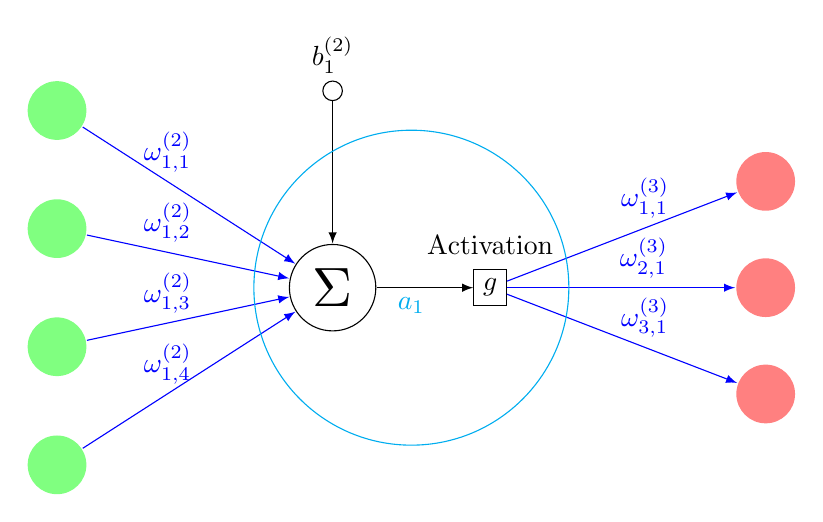
\begin{tikzpicture}[>=latex]
\path
(0,0)     node[circle,draw,scale=2,inner sep=2pt] (S) {$\Sigma$}
+(90:2.5) node[circle,draw,inner sep=2.5pt] (b) {}
          node[above=1mm] {$b_1^{(2)}$}
+(-3.5,2.25)  node[circle,scale=2.25,fill=green!50]  (x1) {} %{$T_{2m}$}
+(-3.5,0.75)  node[circle,scale=2.25,fill=green!50]  (x2) {} %{$q_v$}
+(-3.5,-0.75) node[circle,scale=2.25,fill=green!50]  (x3) {} %{$RH$}
+(-3.5,-2.25) node[circle,scale=2.25,fill=green!50]  (x4) {} %{$p_s$}
(2,0)    node[draw] (g) {$g$} node[above=3mm]{Activation}

+(3.5,1.35)  node[circle,scale=2.25,fill=red!50]  (y1) {}
+(3.5,0)  node[circle,scale=2.25,fill=red!50]  (y3) {}
+(3.5,-1.35) node[circle,scale=2.25,fill=red!50]  (y2) {};

\draw[->, black] (S)--(g);
\draw[->, black] (b)--(S);
\draw[->, blue] (g)--(y1) node[pos=.6,above, blue]{$\omega_{1,1}^{(3)}$};
\draw[->, blue] (g)--(y2) node[pos=.6,above, blue]{$\omega_{3,1}^{(3)}$};
\draw[->, blue] (g)--(y3) node[pos=.6,above, blue]{$\omega_{2,1}^{(3)}$};

\draw[->, blue] (x1)--(S) node[pos=.4,above, blue]{$\omega_{1,1}^{(2)}$};
\draw[->, blue] (x2)--(S) node[pos=.4,above, blue]{$\omega_{1,2}^{(2)}$};
\draw[->, blue] (x3)--(S) node[pos=.4,above, blue]{$\omega_{1,3}^{(2)}$};
\draw[->, blue] (x4)--(S) node[pos=.4,above, blue]{$\omega_{1,4}^{(2)}$};
\draw[cyan] (1,0) circle(2) node[below]{$a_1$};
\end{tikzpicture}

\caption{Computational graph showing the components participating in the activation of a neuron in the hidden layer. This example shows a 2-layer neural network with four input nodes and three output nodes. The number of nodes in the hidden layer doesn't affect the activation, because they are not connected. The sum of the weighted inputs and the bias is passed to the activation function, inside the hidden layers, producing the activation of the neuron. This is again passed to the output neurons. Modified sketch based on example from \citepaper{activation_one_node}. %\href{https://tex.stackexchange.com/questions/505741/architecture-neural-network-with-weights}{https://tex.stackexchange.com/questions/505741/architecture-neural-network-with-weights}. 
}
\label{fig:activation_one_node}
\end{figure}

Figure \ref{fig:activation_one_node} shows the computation which takes place in a node in the hidden layer, a dot the middle column in Figure \ref{fig:one_layer_mlp}. The sum of the weighted input and bias are sent trough the activation function, $g$, producing the activation. The activation function is a hyperparameter, set before the training starts. Popular choices are rectified linear unit (ReLU), sigmoid or tanh-function. These are shown in Figure \ref{fig:activation_function_example}.
\begin{figure}
    \centering
    \includegraphics[scale = 0.4]{Chapter3_Method/figs/activation_functions_and_derivatives.png}
    \caption{Activation functions and their derivatives.}
    \label{fig:activation_function_example}
\end{figure}
Equation \eqref{eq:activation_hidden_pass} describes the activation of a node in a arbitrary layer, L. $b_L$ denotes the bias, $w_L$ is the weights matrix. and $n$ is the number of input nodes. $g_h$ denotes activation function in hidden layer and $g_o$ is the activation function chosen for the output layer. For regression problem, $g_o$ is linear like.
\begin{equation} \label{eq:activation_hidden_pass}
    \textbf{a}_L = g_h(\sum_{i=1}^n \textbf{W}_{L, i} \textbf{x}_i + b_L)
\end{equation}
\begin{equation} \label{eq:output_pass}
    \textbf{a}_{L+1} = g_o(\sum_{i=1}^n \textbf{W}_{L+1, i} \textbf{a}_{L+1} + b_{L+1})
\end{equation}
\textbf{Thought to self, Notation is trick when the next layer is the output. Since the activation-function usually is different in hidden layers and output layers. }
% Recursively moving things to next layer.
The activation's of the first layer is weighted, and passed to the output layer, according to Equation \eqref{eq:output_pass}.

\subsection{Convolutional neural networks} \label{sec:convolutional neural network}
%\textit{According to the philosophy underlying deep learning approach, if we have a reasonable end-to-end model and a sufficient data for training it, we are close to solving the problem}. (Shi et. al., 2015). 

Computer vision is a field of artificial intelligence concerned with interpreting the visual world. One popular structure for visual tasks is the convolutional neural network. %Its said to resemble the visual cortex, the centre in the brain which processes the visual information. 
\begin{figure}[h] % h means place here if possible
    \centering
    \begin{tikzpicture}[scale=1.5,every node/.style={minimum size=1cm}, on grid]
    % slanting: production of a set of n 'laminae' to be piled up.
    % N=number of grids.
    
            
        \begin{scope}[yshift=-200, xshift = -200, 
                      every node/.append style={yslant=0.,xslant=0},
                      yslant=0,xslant=0]
            \draw[black, very thick, fill = gray, opacity = 0.2] (0,0) rectangle (2.8, 3.6);
            \draw[step = 4mm, very thick, black] (0,0) grid (2.8, 3.6);
            \coordinate (s9) at (0.2, 3.4);
            \node at (s9) [circle, scale=1.5] {$P$};
            
        \end{scope} 
        
    
        % RED LAYER 
        \begin{scope}[yshift=-200,every node/.append style={
            yslant=0.5,xslant=-1.3},yslant=0.5,xslant=-1.3 ]
            \draw[black, very thick, fill = red, opacity = 0.2] (0,0) rectangle (2.1, 2.7); % marking borders 
            \draw[black, very thick] (0,0) rectangle (2.1, 2.7); % marking borders
            
            \coordinate (s9) at (0, 0);
            \coordinate (s10) at (0, 2.7);
            \coordinate (s11) at (2.1, 0);
            \coordinate (s12) at (2.1, 2.7);

            \coordinate (t1) at (0, 0.3);
            %\node at (t1) [circle, fill = blue, scale=.5] {$P$};
            
            \coordinate (t2) at (0, 0.6);
            %\node at (t2) [circle, fill = blue, scale=.5] {$P$};
            
            \coordinate (t3) at (0, 0.9);
            %\node at (t3) [circle, fill = blue, scale=.5] {$P$};
            
            \coordinate (t4) at (0, 1.2);
            %\node at (t4) [circle, fill = blue, scale=.5] {$P$};
            
            \coordinate (t5) at (0, 1.5);
            %\node at (t5) [circle, fill = blue, scale=.5] {$P$};
            
            \coordinate (t6) at (0, 1.8);
            %\node at (t6) [circle, fill = blue, scale=.5] {$P$};
            
            \coordinate (t7) at (0, 2.1);
            %\node at (t7) [circle, fill = blue, scale=.5] {$P$};
            
            \coordinate (t8) at (0, 2.4);
            %\node at (t8) [circle, fill = blue, scale=.5] {$P$};
            
            \coordinate (t9) at (0.3, 0);
            %\node at (t9) [circle, fill = blue, scale=.5] {$P$};
            
            \coordinate (t10) at (0.6, 0);
            %\node at (t10) [circle, fill = blue, scale=.5] {$P$};
            
            \coordinate (t11) at (0.9, 0);
            %\node at (t11) [circle, fill = blue, scale=.5] {$P$};
            
            \coordinate (t12) at (1.2, 0);
            %\node at (t12) [circle, fill = blue, scale=.5] {$P$};
            
            \coordinate (t13) at (1.5, 0);
            %\node at (t13) [circle, fill = blue, scale=.5] {$P$};
            
            \coordinate (t14) at (1.8, 0);
            %\node at (t14) [circle, fill = blue, scale=.5] {$P$};

            
        \end{scope} 
        
        
        \begin{scope}[
            yshift=-195,every node/.append style={
            yslant=0.5,xslant=-1.3},yslant=0.5,xslant=-1.3
                      ]
            \draw[black, very thick, fill = green, opacity = 0.2] (0,0) rectangle (2.1, 2.7); % marking borders 
            \coordinate (h_input) at (2.1, 0);
            \coordinate (h_bl) at (0, 2.7);
            %\node at (h_bl) [fill=blue, circle, scale=0.5] {$s$};
        \end{scope} 
        
        % BLUE LAYER 
        \begin{scope}[yshift=-190,every node/.append style={
                yslant=0.5,xslant=-1.3},yslant=0.5,xslant=-1.3]
                \draw[black, very thick, fill = blue, opacity = 0.2] (0,0) rectangle (2.1, 2.7); % marking borders 
                \draw[black, very thick] (0,0) rectangle (2.1, 2.7); % marking borders 
                %\draw[black, very thick] (0,0) rectangle (2.1, 2.7); % marking borders 
                \draw[step=3mm, very thick, black] (0, 0) grid (2.1, 2.7);
                
                \coordinate (s1) at (0, 0);
                \coordinate (s2) at (0, 2.7);
                \coordinate (s3) at (2.1, 0);
                \coordinate (s4) at (2.1, 2.7);
    
                \draw[black,very thick]   (s9) -- (s1);
                \draw[black,very thick]   (s10) -- (s2);
                \draw[black,very thick]   (s11) -- (s3);
                \draw[black,very thick]   (s12) -- (s4);
                
                \coordinate (s9) at (0.15, 2.55);
                \node at (s9) [circle, scale=1.5] {$P$};
                
            \coordinate (h1) at (0, 0.3);
            %\node at (t1) [circle, fill = blue, scale=.5] {$P$};
            
            \coordinate (h2) at (0, 0.6);
            %\node at (t2) [circle, fill = blue, scale=.5] {$P$};
            
            \coordinate (h3) at (0, 0.9);
            %\node at (t3) [circle, fill = blue, scale=.5] {$P$};
            
            \coordinate (h4) at (0, 1.2);
            %\node at (t4) [circle, fill = blue, scale=.5] {$P$};
            
            \coordinate (h5) at (0, 1.5);
            %\node at (t5) [circle, fill = blue, scale=.5] {$P$};
            
            \coordinate (h6) at (0, 1.8);
            %\node at (t6) [circle, fill = blue, scale=.5] {$P$};
            
            \coordinate (h7) at (0, 2.1);
            %\node at (t7) [circle, fill = blue, scale=.5] {$P$};
            
            \coordinate (h8) at (0, 2.4);
            %\node at (t8) [circle, fill = blue, scale=.5] {$P$};
            
            \coordinate (h9) at (0.3, 0);
            %\node at (t9) [circle, fill = blue, scale=.5] {$P$};
            
            \coordinate (h10) at (0.6, 0);
            %\node at (t10) [circle, fill = blue, scale=.5] {$P$};
            
            \coordinate (h11) at (0.9, 0);
            %\node at (t11) [circle, fill = blue, scale=.5] {$P$};
            
            \coordinate (h12) at (1.2, 0);
            %\node at (t12) [circle, fill = blue, scale=.5] {$P$};
            
            \coordinate (h13) at (1.5, 0);
            %\node at (t13) [circle, fill = blue, scale=.5] {$P$};
            
            \coordinate (h14) at (1.8, 0);
            %\node at (t14) [circle, fill = blue, scale=.5] {$P$};
                
        \end{scope}
        
        \draw[black,very thick]   (t1) -- (h1);
        \draw[black,very thick]   (t2) -- (h2);
        \draw[black,very thick]   (t3) -- (h3);
        \draw[black,very thick]   (t4) -- (h4);
        \draw[black,very thick]   (t5) -- (h5);
        \draw[black,very thick]   (t6) -- (h6);
        \draw[black,very thick]   (t7) -- (h7);
        \draw[black,very thick]   (t8) -- (h8);
        \draw[black,very thick]   (t9) -- (h9);
        \draw[black,very thick]   (t10) -- (h10);
        \draw[black,very thick]   (t11) -- (h11);
        \draw[black,very thick]   (t12) -- (h12);
        \draw[black,very thick]   (t13) -- (h13);
        \draw[black,very thick]   (t14) -- (h14);
    
    
    \end{tikzpicture}    
    
    \caption{Transforming t 2D image to a 3D tensor. Decoding a image into RGB (red green blue) channels. Inspired by Figure 1 in \cite{precip_nowcasting}.}
    \label{fig:2D_image}
\end{figure}
Computers see images as a grid of numbers, often decoded in red, green and blue (RGB) channels. Figure \ref{fig:2D_image} shows the transformation of a two-dimensional image to a 3-dimensional tensor. The ``P'' shows the connection between one pixel (``picture element'') and a volume. Each of the grid cells (pixels) contains the signal from the color decoded into values ranging from 0 to 255. The machine needs to learn how to extract the necessary information about these pixels to perform a task. More layers increase the model's ability to extract these complex structures, resulting in an improved model performance. 

% kilde https://tex.stackexchange.com/questions/522118/visualizing-matrix-convolution 
\begin{figure}[hp]
    \centering
    \begin{tikzpicture}[mmat/.style={matrix of math nodes,column sep=-\pgflinewidth/2,
   row sep=-\pgflinewidth/2,cells={nodes={draw,inner sep=2pt,thin}},draw=#1,thick, inner sep=0pt},
   mmat/.default=green,
   node distance=0.3em]
   
 \matrix[mmat](mat1){
         0 & 1 & 1 & |[draw=green,thick,fill=green!20,alias=1]| 1 & |[draw=green,thick,fill=green!20,alias=0]| 0 & |[draw=green,thick,fill=green!20,alias=]| 0 & 0 \\ 
         0 & 0 & 1 & |[draw=green,thick,fill=green!20,alias=1]|1 & |[draw=green,thick,fill=green!20,alias=1]|1 &|[draw=green,thick,fill=green!20,alias=0]| 0 & 0 \\ 
         0 & 0 & 0 & |[draw=green,thick,fill=green!20,alias=1]|1 &|[draw=green,thick,fill=green!20,alias=1]| 1 & |[draw=green,thick,fill=green!20,alias=1]|1 & 0 \\ 
         0 & 0 & 0 & 1 & 1 & 0 & 0 \\ 
         0 & 0 & 1 & 1 & 0 & 0 & 0 \\ 
         0 & 1 & 1 & 0 & 0 & 0 & 0 \\ 
         0 & 1 & 0 & 0 & 0 & 0 & 0 \\ 
         };
 \node[fit=(mat1-1-4)(mat1-3-6),inner sep=0pt, draw, green, thick, fill = green, opacity = 0.2](f1){};        
 
 \node[right=of mat1] (mul) {$*$};      
 \matrix[mmat=blue,fill=blue!30,right=of mul](mat2){    
     1 & 0 & 1 \\ 
     0 & 1 & 0 \\ 
     1 & 0 & 1 \\ };
 \node[right=of mat2] (eq) {$=$};       
 \matrix[mmat,right=of eq, draw = red](mat3){    
     1 & 4 & 3 & |[draw=red,thick,fill=red!20,alias=4]|4 & 1 \\ 
     1 & 2 & 4 & 3 & 3 \\ 
     1 & 2 & 3 & 4 & 1 \\ 
     1 & 3 & 3 & 1 & 1 \\ 
     3 & 3 & 1 & 1 & 0 \\ 
 };
 \foreach \Anchor in {south west,north west,south east,north east}
 {\draw[blue,densely dotted] (f1.\Anchor) -- (mat2.\Anchor); 
 \draw[red,densely dotted] (4.\Anchor) -- (mat2.\Anchor);}
 \begin{scope}[on background layer]
  \fill[red!20] (f1.north west) rectangle (f1.south east);
 \end{scope}
\end{tikzpicture}
    \caption{Diagram showing a convolutional operation. Modified sketch based on \cite{convolution_operation}.}
    \label{fig:convolution}
\end{figure}
Figure \ref{fig:convolution} shows the mathematical operation convolution as the sum over element-wise multiplication of the filter and input. The filter is blue, this is placed over the filled green section, producing the red output pixel. The entire red grid is called a feature map (output map). The green grid is the input, overlaid with blue illustrated the pixels contributing to the activation, red pixel. In Figure \ref{fig:convolution} this would be the value 4. \textit{Receptive field} is known as the pixels contributing to the activation in a pixel (i.e. the value). For instance the receptive field of the shaded red pixel is the shaded green submatrix.


\begin{figure}[h] % h means place here if possible
    \centering
    \begin{tikzpicture}[scale=1.75,every node/.style={minimum size=1cm},on grid]
    % slanting: production of a set of n 'laminae' to be piled up.
    % N=number of grids.
    \begin{scope}[
            yshift=-100, xshift= 0, every node/.append style={
            yslant=0.5, xslant=-1.3}, yslant=0.5, xslant=-1.3
            ]
        % opacity to prevent graphical interference
        \draw[red, very thick, fill = white]  (0, 0) rectangle (1.5, 2.1);
        \draw[step=3mm, thin, red] (0, 0) grid (1.5, 2.1);   % defining grids
        \draw[red, very thick] (0, 0) rectangle (1.5, 2.1); % marking borders    
        
        % pixel closest to output layes
        \coordinate (bl) at (0.16, 1.92);
        \node at (bl) [fill=red!80,   scale=0.65] {};
        
        %last pixel
        \coordinate (pi) at (0.5, 1.92);
        \node at (pi) [fill=red!60,   scale=0.65] {};
        
        % rightmost pixel
        \coordinate (cy) at (0.16, 0.16);
        \node at (cy) [fill=red!40,   scale=0.64] {};
        
        \coordinate (input_c) at (0, 2.1);
        %\node at (corner) [fill=yellow,   scale=0.64] {s};        
        
        \end{scope}
    
        \begin{scope}[
            yshift=-160,every node/.append style={
            yslant=0.5,xslant=-1.3},yslant=0.5,xslant=-1.3
                      ]
            % Marking border
            \draw[blue, very thick, fill = gray!70] (0,0) rectangle (2.1, 2.7);
            \draw[green, very thick, fill = green!20] (0.33, 0.33) rectangle (1.8, 2.4);
            \draw[step=3mm, thin, gray] (0,0) grid   (2.1, 2.7);  % defining grid padding
            \draw[step=3mm, thick, green] (0.33, 0.33) rectangle (1.8, 2.4); % defining grids
            \draw[black, very thick] (0,0) rectangle (2.1, 2.7);% marking borders   
            % \draw[black,very thick, fill = blue!50] (0,0) rectangle (3,3);

            \coordinate (s1) at (0, 2.7);
            %\node at (s1) [fill=blue, circle, scale=0.5] {$s$};
            \coordinate (s2) at (0, 1.8);
            %\node at (s2) [fill=pink, circle, scale=0.5] {$s$};
            \coordinate (s3) at (0.9, 1.8);
            %\node at (s3) [fill=yellow, circle, scale=0.5] {$s$};
            \coordinate (s4) at (0.9, 2.7);
            %\node at (s4) [fill=blue, circle, scale=0.5] {$s$};
                      
            \draw[draw=blue, very thick, line join=round, dashed, fill = blue, opacity = 0.5] %  opacity=.2, 
                  (0,  2.7) -- 
                  (0,  1.8) --
                  (0.9,  1.8) --
                  (0.9,  2.7) -- cycle ;
                
            \draw[fill=white, draw=blue, opacity=.5, very thick, line join=round]
            (s4) -- (bl);
            
            \draw[fill=white, draw=blue, opacity=.5, very thick, line join=round]
            (s3) -- (bl);
 
            \draw[fill=white, draw=blue, opacity=.5, very thick, line join=round]
            (s2) -- (bl);
            
            \draw[fill=white, draw=blue, opacity=.5, very thick, line join=round]
            (s1) -- (bl);
           
           %%%%%%%%%%%%%%%%%%%%%%%% PINK
            \coordinate (s5) at (0.333, 2.7);
            %\node at (s5) [fill=blue, circle, scale=0.5] {$s$};

            \coordinate (s6) at (0.333, 1.8);
            %\node at (s6) [fill=pink, circle, scale=0.5] {$s$};

            \coordinate (s7) at (1.2333, 1.8);
            %\node at (s7) [fill=yellow, circle, scale=0.5] {$s$};

            \coordinate (s8) at (1.2333, 2.7);
            %\node at (s8) [fill=blue, circle, scale=0.5] {$s$};
           
           
           
            \draw[draw=blue, very thick, line join=round, opacity=.2, fill = blue, opacity = 0.5] %  opacity=.2, 
                  (s5) -- (s6) -- (s7) -- (s8) -- cycle;

            \draw[fill=white, draw=blue, opacity=0.5, very thick, line join=round, dashed]
            (s5) -- (pi);
            
            \draw[fill=white, draw=blue, opacity=0.5, very thick, line join=round, dashed]
            (s6) -- (pi);
 
            \draw[fill=white, draw=blue, opacity=.5, very thick, line join=round, dashed]
            (s7) -- (pi);
            
            \draw[fill=white, draw=blue, opacity=.5, very thick, line join=round, dashed]
            (s8) -- (pi);
            
            %%%%%%%%%%%%%%%%%%%%%%%% blue
            \coordinate (s9) at (0, 0);
            %\node at (s5) [fill=blue, circle, scale=0.5] {$s$};

            \coordinate (input_layer) at (0.32, 1);
            %\node at (input_layer) [fill=blue, circle, scale=0.5] {$s$};

            \coordinate (s10) at (0, 0.9);
            %\node at (s6) [fill=pink, circle, scale=0.5] {$s$};

            \coordinate (s11) at (0.9, 0.9);
            %\node at (s7) [fill=yellow, circle, scale=0.5] {$s$};

            \coordinate (s12) at (0.9, 0);
            %\node at (s8) [fill=blue, circle, scale=0.5] {$s$};
           
            % Adding coordinates for padding
            \coordinate (p1) at (2.1, 0);
            \coordinate (p2) at (1.8, 0);

            \draw[draw=blue!60, very thick, line join=round, dashed, opacity=.6, fill = blue!60] %  opacity=.2, 
                  (s9) -- (s10) -- (s11) -- (s12) -- cycle;

            \draw[fill=white, draw=blue!60, opacity=.6, very thick, line join=round]
            (s9) -- (cy);
            
            \draw[fill=white, draw=blue!60, opacity=.6, very thick, line join=round]
            (s10) -- (cy);
 
            \draw[fill=white, draw=blue!60, opacity=.6, very thick, line join=round]
            (s11) -- (cy);
            
            \draw[fill=white, draw=blue!60, opacity=.6, very thick, line join=round]
            (s12) -- (cy);
            
        \end{scope} %end of drawing grids
    
       \draw[-latex,thick](-1, -6)node[left, scale=1.]{\small Input layer}
             to[out=0, in=90] (input_layer);  	
            
        \draw[-latex,thick](2.7, -4.25)node[above, scale=1.]{\small Zero padding}
             to[out=0, in=90] (p1);  
        \draw[-latex,thick](2.7, -4.25)node[above, scale=1.]{}
             to[out=0, in=90] (p2);      
             
       \draw[-latex,thick](-3, -2.5)node[left, scale=1.]{\small  Output layer}
             to[out=0,in=90] (input_c);  	
        
        \draw[-latex,thick](-4, -5)node[left, scale=1.]{\small  $f_w = 3$}
               to[out=0,in=90] (s1);  	
        \draw[-latex,thick](-4, -5)node[left]{}
              to[out=0,in=90] (s2);  	
            
        \draw[-latex,thick](-3.7, -4.4)node[left, scale=1.]{\small $f_h = 3$}
               to[out=0,in=90] (s1);  	
        \draw[-latex,thick](-3.7, -4.4)node[left]{}
              to[out=0,in=90] (s4);  
    \end{tikzpicture}
    \caption{The illustration shows the connections between input and output layer. This example uses a $3\times 3$-filter (blue), zero-padding (gray) resulting in equal dimensions for input (green) and output (red). The different colors illustrate the connections between input and output pixels. The input pixels contributing to the output, is called the receptive field. The zero padding is added to keep the input shape. Inspired by Figure (13-3) in \cite{OReiley_book}. 
    }
    \label{fig:convolution_padding}
\end{figure}

Convolving a filter over the input image generates a feature map. If it happens to be the last layer, it is common to refer to the results as the output instead, even though there is no difference. Figure \ref{fig:convolution_padding} shows a 2D-convolution with filter of size $3\times 3$. Filters are often square (not a strict requirement) and the height, $f_h$ and $f_w$ are odd numbers (not a strict requirement either). The origin is the position of the kernel which is above the current output pixels. The connections between the layers are intended to illustrate the part contributing to the pixel, as well as highlighting the receptive field. In order to include the outermost pixels, the input area is padded with zeros around the edges (shown as gray in the figure). 
\begin{figure}
    \centering
   \begin{tikzpicture}[scale=1.5,every node/.style={minimum size=1cm},on grid]
    % slanting: production of a set of n 'laminae' to be piled up.
    % N=number of grids.

        \begin{scope}[
            yshift=-200,every node/.append style={
            yslant=0.5,xslant=-1.3},yslant=0.5,xslant=-1.3
                      ]
            \draw[black, very thick, fill = red, opacity = 0.2] (0,0) rectangle (2.1, 2.7); % marking borders 
            \draw[black, very thick] (0,0) rectangle (2.1, 2.7); % marking borders 

            \coordinate (s9) at (0, 0);
            %\node at (s9) [fill=blue, circle, scale=0.5] {$s$};
            \coordinate (s10) at (0, 2.7);
            %\node at (s10) [fill=pink, circle, scale=0.5] {$s$};
            \coordinate (s11) at (2.1, 0);
            %\node at (s11) [fill=yellow, circle, scale=0.5] {$s$};
            \coordinate (s12) at (2.1, 2.7);
            %\node at (s12) [fill=cyan, circle, scale=0.5] {$s$};
            \coordinate (h_re) at (0, 2.7);
            %\node at (h_re) [fill=red, circle, scale=0.5] {$s$};
                                   
            % begynner i punkt (x, y) rectangle (x dim, y dim)
            \draw[black, very thick, dashed] (0.5, 0.95) rectangle (1.25, 1.25);
            \coordinate (o1) at (0.5, 0.95);
            %\node at (p1) [draw=black, very thick, circle, scale=0.3] {};
            \coordinate (o2) at (0.5, 0.95+1.25/2);
            %\node at (p2) [draw=black, very thick, circle, scale=0.3] {};
            \coordinate (o3) at (0.5+1.25/2+0.1, 0.95);
            %\node at (p3) [draw=black, very thick, circle, scale=0.3] {};
            \coordinate (o4) at (0.5+1.25/2+0.1, 0.95+1.25/2);
            %\node at (p4) [draw=black, very thick, circle, scale=0.3] {};

           
            % begynner i punkt (x, y) rectangle (x dim, y dim)
            \draw[black, very thick, dashed] (0.5, 0.95) rectangle (1.25, 1.6);
            \coordinate (z1) at (0.5, 0.95);
            %\node at (q1) [draw=black, very thick, circle, scale=0.3] {};
            \coordinate (z2) at (0.5, 0.95+1.25/2);
            %\node at (q2) [draw=black, very thick, circle, scale=0.3] {};
            \coordinate (z3) at (0.5+1.25/2+0.1, 0.95);
            %\node at (q3) [draw=black, very thick, circle, scale=0.3] {};
            \coordinate (z4) at (0.5+1.25/2+0.1, 0.95+1.25/2);
            %\node at (q4) [draw=black, very thick, circle, scale=0.3] {};


            %\draw[black, very thick, dashed] (0.8, 0.45) rectangle (1.25, 1.6);
            \coordinate (x1) at (0.8, 0.45);
            %\node at (u1) [draw=black, very thick, circle, scale=0.3] {};
            \coordinate (x2) at (0.8, 0.45+1.25/2);
            %\node at (u2) [draw=black, very thick, circle, scale=0.3] {};
            \coordinate (x3) at (0.8+1.25/2+0.1, 0.45);
            %\node at (u3) [draw=black, very thick, circle, scale=0.3] {};
            \coordinate (x4) at (0.8+1.25/2+0.1, 0.45+1.25/2);
            %\node at (u4) [draw=black, very thick, circle, scale=0.3] {};
            \draw[black,very thick, dashed]   (x1) -- (x3) -- (x4) -- (x2) --(x1);
        \end{scope} 

        \begin{scope}[
            yshift=-195,every node/.append style={
            yslant=0.5,xslant=-1.3},yslant=0.5,xslant=-1.3
                      ]
            \draw[black, very thick, fill = green, opacity = 0.2] (0,0) rectangle (2.1, 2.7); % marking borders 
            \coordinate (h_input) at (2.1, 0);
            \coordinate (h_bl) at (0, 2.7);
            %\node at (h_bl) [fill=blue, circle, scale=0.5] {$s$};
        \end{scope} 
           
           \draw[thick](3, -5.7)node[scale=1.3]{Input Layer};
           \draw[thick](3.5, -3.2)node[scale=1.3]{Convolutional layer 1};
           \draw[thick](3.5, -0.7)node[scale=1.3]{Convolutional layer 2};
           \draw[thick](-4.6, -0.2)node[scale=1.3]{Feature};
           \draw[thick](-4.6, -1.1)node[scale=1.3]{$\vdots$};
           \draw[thick](-4.6, -3.6)node[scale=1.3]{$\vdots$};
           \draw[thick](-4.4, -5.5)node[scale=1.3]{Channels};
           
        \begin{scope}[
            yshift=-190,every node/.append style={
            yslant=0.5,xslant=-1.3},yslant=0.5,xslant=-1.3
                      ]
            \draw[black, very thick, fill = blue, opacity = 0.2] (0,0) rectangle (2.1, 2.7); % marking borders 
            \draw[black, very thick] (0,0) rectangle (2.1, 2.7); % marking borders 

            \coordinate (s1) at (0, 0);
            \coordinate (s2) at (0, 2.7);
            \coordinate (s3) at (2.1, 0);
            \coordinate (s4) at (2.1, 2.7);

            \draw[black,very thick]   (s9) -- (s1);
            \draw[black,very thick]   (s10) -- (s2);
            \draw[black,very thick]   (s11) -- (s3);
            \draw[black,very thick]   (s12) -- (s4);
                        
            \coordinate (h_gr) at (0, 2.7);

            % begynner i punkt (x, y) rectangle (x dim, y dim)
            \draw[black, very thick, dashed] (0.5, 0.95) rectangle (1.25, 1.6);
            \coordinate (q1) at (0.5, 0.95);
            %\node at (q1) [draw=black, very thick, circle, scale=0.3] {};
            \coordinate (q2) at (0.5, 0.95+1.25/2);
            %\node at (q2) [draw=black, very thick, circle, scale=0.3] {};
            \coordinate (q3) at (0.5+1.25/2+0.1, 0.95);
            %\node at (q3) [draw=black, very thick, circle, scale=0.3] {};
            \coordinate (q4) at (0.5+1.25/2+0.1, 0.95+1.25/2);
            %\node at (q4) [draw=black, very thick, circle, scale=0.3] {};

            %\draw[black, very thick, dashed] (0.8, 0.45) rectangle (1.25, 1.6);
            \coordinate (u1) at (0.8, 0.45);
            %\node at (u1) [draw=black, very thick, circle, scale=0.3] {};
            \coordinate (u2) at (0.8, 0.45+1.25/2);
            %\node at (u2) [draw=black, very thick, circle, scale=0.3] {};
            \coordinate (u3) at (0.8+1.25/2+0.1, 0.45);
            %\node at (u3) [draw=black, very thick, circle, scale=0.3] {};
            \coordinate (u4) at (0.8+1.25/2+0.1, 0.45+1.25/2);
            %\node at (u4) [draw=black, very thick, circle, scale=0.3] {};

            \draw[black,very thick, dashed]   (u1) -- (u3) -- (u4) -- (u2) --(u1);

            % Draws horizontal lines completing the litle cube.
            \draw[black,very thick, dashed]   (q1) -- (z1);
            \draw[black,very thick, dashed]   (q2) -- (z2);
            \draw[black,very thick, dashed]   (q3) -- (z3);
            \draw[black,very thick, dashed]   (q4) -- (z4);
            
            % Draws horizontal lines completing the litle cube.
            \draw[black,very thick, dashed]   (u1) -- (x1);
            \draw[black,very thick, dashed]   (u2) -- (x2);
            \draw[black,very thick, dashed]   (u3) -- (x3);
            \draw[black,very thick, dashed]   (u4) -- (x4);
            
        \end{scope} 

        \draw[black, thick, ->](-4.2, -5.95)node[left, scale=1.3]{green} to (h_bl);
        \draw[thick, ->](-4.2, -6.15)node[left, scale=1.3]{red} to (h_re);
        \draw[thick, ->](-4.2, -5.75)node[left, scale=1.3]{blue} to (h_gr);
        %%%%%%%%%%%%%%%%%%%%%%%% END OF INPUT LAYER 


        \begin{scope}[
            yshift=-140, every node/.append style={
            yslant=0.5,xslant=-1.3},yslant=0.5,xslant=-1.3]
            \draw[black, very thick, fill = gray, opacity = 0.2] (0,0) rectangle (2.1, 2.7); % marking borders 
            % Draws the boundary boxes
            \draw[black, very thick] (0,0) rectangle (2.1, 2.7);
            \coordinate (e5) at (0, 0);
            \coordinate (e6) at (0, 2.7);
            \coordinate (e7) at (2.1, 0);
            \coordinate (e8) at (2.1, 2.7);


            % draw left cylinder
            \coordinate (f) at (0.7, 1.1);
            \node at (f) [draw=black, very thick, circle, scale=0.3] {};
            \coordinate (f1) at (0.7, 1.15);
            %\node at (f1) [draw=red, very thick, circle, scale=0.3] {};
            \coordinate (f2) at (0.7, 1.05);
            %\node at (f2) [draw=red, very thick, circle, scale=0.3] {};
            
            % Draws the other
            \coordinate (g) at (1.1, 0.85);
            \node at (g) [draw=black, very thick, circle, scale=0.3] {};
            \coordinate (g1) at (1.1, 0.95);
            \coordinate (g2) at (1.1, 0.8);
            
            % Drawing the smaller lower 
            \draw[black, very thick, dashed] (0.5, 0.65) rectangle (1.25, 1.25);
            \coordinate (o1) at (0.5, 0.65);
            %\node at (o1) [draw=black, very thick, circle, scale=0.3] {};
            \coordinate (o2) at (0.5, 0.65+1.25/2);
            %\node at (o2) [draw=black, very thick, circle, scale=0.3] {};
            \coordinate (o3) at (0.5+1.25/2+0.1, 0.65);
            %\node at (o3) [draw=black, very thick, circle, scale=0.3] {};
            \coordinate (o4) at (0.5+1.25/2+0.1, 0.65+1.25/2);
            %\node at (o4) [draw=black, very thick, circle, scale=0.3] {};
  
        \end{scope} 
        
        \begin{scope}[
            yshift=-135,every node/.append style={
            yslant=0.5,xslant=-1.3},yslant=0.5,xslant=-1.3
                      ]
            \draw[black, very thick, fill = gray, opacity = 0.2] (0,0) rectangle (2.1, 2.7); % marking borders 
        \end{scope} 
    
        \begin{scope}[
            yshift=-130,every node/.append style={
            yslant=0.5,xslant=-1.3},yslant=0.5,xslant=-1.3
                      ]
            \draw[black, very thick, fill = gray, opacity = 0.2] (0,0) rectangle (2.1, 2.7); % marking borders 
        \end{scope} 
    

        \begin{scope}[
            yshift=-125, every node/.append style={
            yslant=0.5,xslant=-1.3},yslant=0.5,xslant=-1.3
                      ]
            \draw[black, very thick, fill = gray, opacity = 0.2] (0,0) rectangle (2.1, 2.7); % marking borders 
            \coordinate (h) at (2.1, 0);
            %\node at (h) [fill=blue, circle, scale=0.5] {$s$};
        \end{scope} 
        
        \begin{scope}[
            yshift=-120,every node/.append style={
            yslant=0.5,xslant=-1.3},yslant=0.5,xslant=-1.3
                      ]
            \draw[black, very thick, fill = gray, opacity = 0.2] (0,0) rectangle (2.1, 2.7); % marking borders 
        \end{scope} 
    
        \begin{scope}[
            yshift=-115,every node/.append style={
            yslant=0.5,xslant=-1.3},yslant=0.5,xslant=-1.3
                      ]
            \draw[black, very thick, fill = gray, opacity = 0.2] (0,0) rectangle (2.1, 2.7); % marking borders 
            
            % Connections to maps
            \coordinate (sec_map_L2) at (0, 2.7);
            %\node at (sec_map_L2) [fill=blue, circle, scale=0.5] {$s$};
            
        \end{scope} 
    
        \begin{scope}[
            yshift=-110,every node/.append style={
            yslant=0.5,xslant=-1.3},yslant=0.5,xslant=-1.3
                      ]
            \draw[black, very thick, fill = gray, opacity = 0.2] (0,0) rectangle (2.1, 2.7); % marking borders 
                    
            % Connections to maps
            \coordinate (sec_map_L1) at (0, 2.7);
            %\node at (sec_map_L1) [fill=blue, circle, scale=0.5] {$s$};
            
          \coordinate (e1) at (0, 0);
          \coordinate (e2) at (0, 2.7);
          \coordinate (e3) at (2.1, 0);
          \coordinate (e4) at (2.1, 2.7);

            \draw[black, very thick] (0,0) rectangle (2.1, 2.7); % draw boundaries
            % draws horizontal lines
            \draw[black,very thick]   (e5) -- (e1);
            \draw[black,very thick]   (e6) -- (e2);
            \draw[black,very thick]   (e7) -- (e3);
            \draw[black,very thick]   (e8) -- (e4);
            
            % begynner i punkt (x, y) rectangle (x dim, y dim)
            \draw[black, very thick, dashed] (0.5, 0.65) rectangle (1.25, 1.25);
            \coordinate (p1) at (0.5, 0.65);
            %\node at (p1) [draw=black, very thick, circle, scale=0.3] {};
            \coordinate (p2) at (0.5, 0.65+1.25/2);
            %\node at (p2) [draw=black, very thick, circle, scale=0.3] {};
            \coordinate (p3) at (0.5+1.25/2+0.1, 0.65);
            %\node at (p3) [draw=black, very thick, circle, scale=0.3] {};
            \coordinate (p4) at (0.5+1.25/2+0.1, 0.65+1.25/2);
            %\node at (p4) [draw=black, very thick, circle, scale=0.3] {};

            % Draws horizontal lines completing the litle cube.
            \draw[black,very thick, dashed]   (p1) -- (o1);
            \draw[black,very thick, dashed]   (p2) -- (o2);
            \draw[black,very thick, dashed]   (p3) -- (o3);
            \draw[black,very thick, dashed]   (p4) -- (o4);
            
            % draw one cylinder
            \coordinate (w) at (0.7, 1.1);
            \node at (w) [draw=black, very thick, circle, scale=0.3] {};
            \coordinate (w1) at (0.7, 1.15);
            %\node at (f1) [draw=red, very thick, circle, scale=0.3] {};
            \coordinate (w2) at (0.7, 1.05);
            %\node at (f2) [draw=red, very thick, circle, scale=0.3] {};
            
            % Draws the other
            \coordinate (r) at (1.1, 0.85);
            \node at (r) [draw=black, very thick, circle, scale=0.3] {};
            \coordinate (r1) at (1.1, 0.95);
            \coordinate (r2) at (1.1, 0.8);

            \draw[black, very thick, dashed]   (f1) -- (w1);
            \draw[black, very thick, dashed]   (f2) -- (w2);

            \draw[black, very thick, dashed]   (g1) -- (r1);
            \draw[black, very thick, dashed]   (g2) -- (r2);


            % Connnection between layers 
            \draw[black,very thick, dashed]   (q1) -- (f);
            \draw[black,very thick, dashed]   (q2) -- (f);
            \draw[black,very thick, dashed]   (q3) -- (f);
            \draw[black,very thick, dashed]   (q4) -- (f);
            
            % Connnection between layers 
            \draw[black,very thick, dashed]   (u1) -- (g);
            \draw[black,very thick, dashed]   (u2) -- (g);
            \draw[black,very thick, dashed]   (u3) -- (g);
            \draw[black,very thick, dashed]   (u4) -- (g);
            

        \end{scope} 
    
    
    
    
    
    %%%%%%%%%%%%%%%%%%%%%%%%%%%%% CONVOLUTIONAL LAYER 2
        
        \begin{scope}[
            yshift=-50,every node/.append style={
            yslant=0.5,xslant=-1.3},yslant=0.5,xslant=-1.3
                      ]
            \draw[black, very thick, fill = gray, opacity = 0.2] (0,0) rectangle (2.1, 2.7); % drawing layer 
            \coordinate (h) at (2.1, 0);
            %\node at (h) [fill=blue, circle, scale=0.5] {$s$};
            
        \end{scope} 

        \begin{scope}[
            yshift=-55,every node/.append style={
            yslant=0.5,xslant=-1.3},yslant=0.5,xslant=-1.3
                      ]
            \draw[black, very thick, fill = gray, opacity = 0.2] (0,0) rectangle (2.1, 2.7); % marking borders 
        \end{scope} 
        
        \begin{scope}[
            yshift=-60,every node/.append style={
            yslant=0.5,xslant=-1.3},yslant=0.5,xslant=-1.3
                      ]
                      
            % The outer box
            \draw[black, very thick, fill = gray, opacity = 0.2] (0,0) rectangle (2.1, 2.7); % marking borders 
            \coordinate (a5) at (0, 0);
            \coordinate (a6) at (0, 2.7);
            \coordinate (a7) at (2.1, 0);
            \coordinate (a8) at (2.1, 2.7);
            \draw[black, very thick] (0,0) rectangle (2.1, 2.7); % draw boundaries
                    
            % The inner box
            \coordinate (h) at (1.1, 1.2); % this should be connected to the next layer
            \node at (h) [draw=black, very thick, circle, scale=0.3] {};
            \coordinate (h1) at (1.1, 1.25);
            \coordinate (h2) at (1.1, 1.15);
            
        \end{scope} 
    
            \begin{scope}[
            yshift=-45,every node/.append style={
            yslant=0.5,xslant=-1.3},yslant=0.5,xslant=-1.3
                      ]
            \draw[black, very thick, fill = gray, opacity = 0.2] (0,0) rectangle (2.1, 2.7); % marking borders 
            
            \coordinate (sec_map) at (0, 2.7);
            %\node at (sec_map) [fill=blue, circle, scale=0.5] {$s$};
            
        \end{scope} 
        
        \begin{scope}[
            yshift=-40,every node/.append style={
            yslant=0.5,xslant=-1.3},yslant=0.5,xslant=-1.3
                      ]
            \draw[black, very thick, fill = gray, opacity = 0.2] (0,0) rectangle (2.1, 2.7); % marking borders 
            \coordinate (a1) at (0, 0);
            \coordinate (a2) at (0, 2.7);
            \coordinate (a3) at (2.1, 0);
            \coordinate (a4) at (2.1, 2.7);

            \draw[black, very thick] (0,0) rectangle (2.1, 2.7); % draw boundaries
            % draws horizontal lines
            \draw[black,very thick]   (a5) -- (a1);
            \draw[black,very thick]   (a6) -- (a2);
            \draw[black,very thick]   (a7) -- (a3);
            \draw[black,very thick]   (a8) -- (a4);
            
            % Draws the cylinder
            \coordinate (i) at (1.1, 1.2);
            \node at (i) [draw=black, very thick, circle, scale=0.3] {};
            \node[right of=i, node distance=0.5cm] (p) {P};
            
            \coordinate (i1) at (1.1, 1.25); % for lines
            \coordinate (i2) at (1.1, 1.15); % for lines
            
            % drawing lines
            \draw[black,very thick, dashed]   (i1) -- (h1);
            \draw[black,very thick, dashed]   (i2) -- (h2);

            % Draw the lines connecting the first and second layer.
            \draw[black,very thick, dashed]   (p1) -- (h);
            \draw[black,very thick, dashed]   (p2) -- (h);
            \draw[black,very thick, dashed]   (p3) -- (h);
            \draw[black,very thick, dashed]   (p4) -- (h);

            \coordinate (first_map) at (0, 2.7);
            %\node at (first_map) [fill=blue, circle, scale=0.5] {$s$};

        \end{scope} 
    
        \draw[thick, ->](-4.2, -0.5)node[left, scale=1.3]{Map 1} to (first_map);
        \draw[thick, ->](-4.2, -0.8)node[left, scale=1.3]{Map 2} to (sec_map);
     
        \draw[thick, ->](-4.2, -3)node[left, scale=1.3]{Map 1} to (sec_map_L1);
        \draw[thick, ->](-4.2, -3.3)node[left, scale=1.3]{Map 2} to (sec_map_L2);
    % signed distance
    \end{tikzpicture}    
    \caption[Receptive field of pixel in convolutional neural network trained on RGB-image.]{First two layers of a convolutional neural network trained on RGB-images. Each convolutional layer contains multiple filters, thus producing stack of feature maps. Each layer learn the representation of the previous layer. The trailing layer get this stack as input, producing activations based on all channels. For each layer it contains representations of the structures found in the previous layer. The filters are the weights trained to find useful structures. In each convolutional layer multiple of these filters are passed over the image. The dashed volumes illustrate the receptive fields of a pixel, ``P''. The receptive field of a node in the second layer is larger than the one in first, since a pixel inherant the receptive fields of the nodes in its receptive field. Inspired by Figure (13-6) in \cite{OReiley_book}.
    }
    \label{fig:conv_layers}
\end{figure} 
It is worth noting that the same structures are given different names, based on their position in the network. The output is the feature map resulting from convolving the last layer. They are both activations, computed from the values and weights from the previous layer. The number of channels in the first layer and the numbers of feature maps in the subsequent layers are both simply stacks of grids containing values.

Working with RGB images requires 3D convolution; since the dimensions of the input determines the dimensions of the convolution, it is commonly referred to as simply convolution. As mentioned earlier, neural networks are strucured as a stack of layers. Each layer is again a stack of channels or feature maps. The output from the previous layer becomes the input to the next layer. Feature maps, activations, and outputs are all the result of a convolution, produced at different points within a neural net. The activations are computed based on an input volume, including information across channels. A 3D convolution collapses information on multiple colors into a single value.

Figure \ref{fig:conv_layers} shows a two layer convolutional neural network trained on RGB-images. The input layer is an RGB-image. The first convolutional layer has seven channels (feature maps), these are produced by seven filters. Filters are trained to extract useful features. The second convolutional layer is produced by five filters, all convolving layer 1. This is a simplified network, made shallow for illustrative purposes. Function CNNs require many layers to extract useful information from an image. %Networks are usually a lot deeper. 
Given raw input (\textit{i.e,} normalized images), the first layers detect low level features like edges, corners and circles. Later layers assemble the features to more complex structures like houses or dogs. The dashed volumes represent the receptive field for different pixels, illustrated as circles. Since each of the layers depend on the previous one, the receptive field of the a node, $P$ depends on a large portion of the input image. Small filters allow you to focus on small features in the data, while larger filters allow you to identify coarser relations.

Unlike fully connected layers (see Figure \ref{fig:one_layer_mlp}), the nodes in the output layer are not connected to all the input nodes, only the nodes within their receptive fields. The filters contain the trained units. Its dimensions determine the size of the feature it can detect. One convolution (using one filter) searches for a single feature over the entire image. When it finds this particular feature it activates, propoagating this signal into the feature maps.% Reduces the number of trainable parameters and making it more robust against overfitting.

\subsection{Recurrent Nets} \label{sec:reccurent_nets}
% Recurrent betyr tilbakevendende
% Sequential modelling has had a great success in applications such as machine translation and speech recognition 
\begin{figure}[h] % h means place here if possible
    \centering
        \begin{tikzpicture}[
    % GLOBAL CFG
    font=\sf \scriptsize,
    >=LaTeX,
    % Styles
    cell/.style={% For the main box
        rectangle, 
        rounded corners=5mm, 
        draw,
        very thick,
        },
    operator/.style={%For operators like +  and  x
        circle,
        draw,
        inner sep=-0.5pt,
        minimum height =.01cm,
        },
    function/.style={%For functions
        ellipse,
        draw,
        inner sep=1pt
        },
    ct/.style={% For external inputs and outputs
        circle,
        draw,
        line width = .75pt,
        minimum width=0.2cm,
        inner sep=1pt,
        },
    gt/.style={% For internal inputs
        rectangle,
        draw,
        minimum width=4mm,
        minimum height=3mm,
        inner sep=1pt
        },
    mylabel/.style={% something new that I have learned
        font=\scriptsize\sffamily
        },
    ArrowC1/.style={% Arrows with rounded corners
        rounded corners=.25cm,
        thick,
        },
    ArrowC2/.style={% Arrows with big rounded corners
        rounded corners=.5cm,
        thick,
        },
    ]

%Start drawing the thing...    
    % Draw the cell: 
    \node [cell, minimum height =1.5cm, minimum width=2cm, fill = cyan!50] (first) at (0,0){\Large \textbf{A}}; % , fill=green

    %\node[ct, label={[mylabel]Cell state}] (c) at (-4,1.5) {\empt{c}{t-1}};
    \node[ct, fill = red!50, scale = 2.25] (h) at (0, 2) {$y_{t}$}; % , fill=blue
    \node[ct, fill = green!50, scale = 2.25] (x) at (0, -2) { $x_t$}; %, fill = magenta
    \draw [->, ArrowC1] (x) -- (first);
    \draw [->, ArrowC1] (first) -- (h);

    %\node [operator, fill = black, opacity = 1] (a) at (0, 1) { };
    %\node [operator, fill = black, opacity = 1] (d) at (-2, 1) { };
    %\node [operator, fill = black, opacity = 1] (c) at (2, 0) { }; 
    %\node [operator, fill = black, opacity = 1] (b) at (-2, .0) { };

    %\draw [->, ArrowC1] (first) -- (a) -- (d) -- (b)  -- (first);
     
    \draw[-latex, thick, white] (first) to[out=110,in=180, loop] node[above] { \Large $h_t$} (first);  %
    \draw[-latex, thick, black] (first) to[out=70,in=360, loop] node[auto] {\Large $h_t$} (first);  

    %\draw [->] (first) to[loop above] node[auto] {} (first);
    \end{tikzpicture}
    
    \caption{Simple one layer recurrent network, $x_t$ denotes the input element of the training sequence, $h_t$ denotes the hidden state, $y_t$ denotes the output of the neuron and A denotes a artificial recurrent unit. In the simplest cases without output activations the hidden state and the output is identical. Inspired by \cite{colah_blog_post}.}
    \label{fig:rnn}
\end{figure}
A recurrent neural network (RNN) is a class of artificial neural networks developed for studying patterns in sequential data such as time series, audio, or text. Figure \ref{fig:rnn} shows the structure of a simple RNN. In very simplified terms, a RNN receives an input, produces an output and passes hidden state back to itself. In Figure \ref{fig:rnn}, A denotes a recurrent unit, $x_t$ denotes the input data and  $h_t$ denotes the hidden state. The output from an arbitrary node, $t$ is $y_t$. %The loop explains the origin of the name recurrent neural network. 
The hidden state contains the information about what you have learned so far. The output at each time step is dependent on the previous inputs. 

\begin{figure}[h] % h means place here if possible
    \centering
        \begin{tikzpicture}[
    % GLOBAL CFG
    font=\sf \scriptsize,
    >=LaTeX,
    % Styles
    cell/.style={% For the main box
        rectangle, 
        rounded corners=5mm, 
        draw,
        very thick,
        },
    operator/.style={%For operators like +  and  x
        circle,
        draw,
        inner sep=-0.5pt,
        minimum height =.2cm,
        },
    function/.style={%For functions
        ellipse,
        draw,
        inner sep=1pt
        },
    ct/.style={% For external inputs and outputs
        circle,
        draw,
        line width = .75pt,
        minimum width=1cm,
        inner sep=1pt,
        },
    gt/.style={% For internal inputs
        rectangle,
        draw,
        minimum width=4mm,
        minimum height=3mm,
        inner sep=1pt
        },
    mylabel/.style={% something new that I have learned
        font=\scriptsize\sffamily
        },
    ArrowC1/.style={% Arrows with rounded corners
        rounded corners=.25cm,
        thick,
        },
    ArrowC2/.style={% Arrows with big rounded corners
        rounded corners=.5cm,
        thick,
        },
    ]

%Start drawing the thing...    
    % Draw the cell: 
    \node [cell, minimum height =1.5cm, minimum width=2cm, fill=cyan!50] (first) at (-1.0, 0){\Large \textbf{A}}; 
    \node [cell, minimum height =1.5cm, minimum width=2cm, fill=cyan!50] (second) at (2.5, 0){\Large \textbf{A}};
    \node [cell, minimum height =1.5cm, minimum width=2cm, fill=cyan!50] (third) at (6,0){\Large \textbf{A}};
    \node [cell, minimum height =1.5cm, minimum width=2cm, fill=cyan!50] (fourth) at (11,0){\Large \textbf{A}};

% Start connecting all.
    %Intersections and displacements are used. 
    % Drawing arrows    
    %\draw [->, ArrowC1] (first) -- (second);
    %\draw [->, ArrowC1] (second) -- (third);
    %\draw [->, ArrowC1] (third) -- (fourth);
    %\draw [->, ArrowC1] (first) -- (second);

    %\node[ct, label={[mylabel]Cell state}] (c) at (-4,1.5) {\empt{c}{t-1}};
    \node[ct, label={[mylabel]Output}, fill = red!50] (h) at (-1, 2) {\large $y_{0}$}; % , fill=blue
    \node[ct, label={[mylabel]below:Input}, fill = green!50] (x) at (-1, -2) {\large $x_0$}; %, fill = magenta
    \draw [->, ArrowC1] (x) -- (first);
    \draw [->, ArrowC1] (first) -- (h);

    %\draw [->, ArrowC1] (first -| first)++(1.5,0) -| (first); 
    %\draw [->, ArrowC1] (h -| ht)++(-0.5,0) -| (ht);
    %\draw [->, ArrowC1] (h -| ht)++(-0.5,0) -| (ht);
    %\draw [->, ArrowC1] (h -| ht)++(-0.5,0) -| (ht);
    
    \node[ct, label={[mylabel]Output}, fill = red!50] (h2) at (2.5, 2) {\large $y_{1}$};
    \node[ct, label={[mylabel]below:Input}, fill = green!50] (x2) at (2.5, -2) {\large $x_1$};
    \draw [->, ArrowC1] (x2) -- (second);
    \draw [->, ArrowC1] (second) -- (h2);
    
    \node[ct, label={[mylabel]Output},  fill = red!50] (h3) at (6, 2) {\large $y_{2}$};
    \node[ct, label={[mylabel]below:Input}, fill = green!50] (x3) at (6, -2) {\large $x_2$};
    \draw [->, ArrowC1] (x3) -- (third);
    \draw [->, ArrowC1] (third) -- (h3);
    
    \node[ct, label={[mylabel]Output},  fill = red!50] (ht) at (11, 2) {\large $y_{t}$};
    \node[ct, label={[mylabel]below:Input}, fill = green!50] (xt) at (11 , -2) {\large $x_t$};
    \draw [->, ArrowC1] (xt) -- (fourth);
    \draw [->, ArrowC1] (fourth) -- (ht);  
    
    \path[->, thick, black] (first) edge [out=90, in=180] node[above, midway] {\Large $h_0$} (second) ;
    \path[->, thick, black] (second) edge [out=90, in=180] node[above, midway] {\Large $h_1$} (third);
    \path[->, thick, gray, dashed] (third) edge [out=90, in=180] node[above, midway] {} (fourth);
    %\path[->, thick, black] (third) edge [out=90, in=180] (fourth);
    
    %\draw (first) to [out=0, in=0,looseness=8] (first);
    \end{tikzpicture}
    
    \caption{Unrolling Figure \ref{fig:rnn} in time, $t$ denotes the length of the training sequence, the elements $x_t$ are the  Inspired by \cite{colah_blog_post}. % Used code from lstm unit to develop this one.
    }
    \label{fig:rnn_unrolled}
\end{figure}
Figure \ref{fig:rnn_unrolled} shows the recurrent network unrolled in time. This way of structuring it resembles the earlier structures like ANN (see figure \ref{fig:one_layer_mlp}). The connection between the nodes %in this kind of networks 
are a directed graph along a temporal sequence. The hidden state from the previous step is fed into the next. $h_0$ is only dependant on $x_0$, while $h_t$ is dependent on $x_0, x_1, \cdots, x_t $. This example shows a one layer recurrent network. All time steps are passed through the same node. The RNN reuses the weights on the input and hidden states for all time steps. Let t denotes the length of the training sequence. The "memory" stores the useful information from $x_0, x_1, \cdots, x_t $ needed to make a prediction, performing the same task on all inputs along the sequence. This reduces the complexity of parameters and in turn lowers the risk of overfitting, obtaining a more general relation between input and output.
% It is used to predict the next word in a sentence or the next tone in a song.  
%%%%%%%%%%%%%%%%%%%%%%%%%%%%%%%%%%%%%%%%%%%%%%%%%%%%%%%%%%%%%%%%%%%%%%%%%%%%%%%%%%%%%
Learning long term dependencies can be a challenging. Learning is done by backpropagating the error signal thought the network. Working with longer sequences, the error signal tends to approach zero or infinity. Exploding gradients can cause the weights to oscillate. Learning from small or vanishing gradients takes ages, or might not learn anything at all. 
%More advanced forms of recurrent nets control the information flow using gates. \textbf{cite 1997 and cite 1999 learning to forget.}

\subsubsection{Long Short-term memory network, LSTM} \label{sec:lstm}
%\textbf{Use recurrent self-connections instead of loops} \textcolor{red}{Ufullstendig setning}.
In order to address challenges in predicting long sequences presented in the previous section, Sepp Hochreiter and Jürgen Schmidhuber created the LSTM network. Their design, documented in a 1997 paper (\textbf{citation)}, outperformed previous memory networks by regulating the flow of information provided to a recurrent network at each time step.
%The memory unit introduced by Sepp Hochreiter and Jürgen Schmidhuber in 1997 set performance records in multiple domains. The paper introduces gates to regulate the flow of information. 
A gate is structure that can be opened or closed. Having values in the range zero to one, it truncates the noise signal from the input and the output. They propose a new method for learning %an approach for constant error flow 
in order to alleviate the issues with exploding or vanishing gradients. The original memory cell contains input and output gates. Gers et. al. 1999 proposed to add an additional gate, the forget gate. The idea was to enable the LSTM to reset parts its own memory. Resetting these parts releases internal resources and enables you to learn even more. 

Because of the interdisciplinary nature of this thesis, this section provides a thorough walk through the LSTM cell and its relevant equations. The memory unit is displayed in Figure \ref{fig:lstm_unit}. The legend describing the different components of the computational graph is available in Figure \ref{fig:legend_lstm}. The information flow thought the cell is regulated by three gates; the forget gate, the input gate and the output gate. These gates are neural networks. The forget gate learns which part of the cell state (the long-term memory) it should forget. The input gate learns the information from the input it should add to the cell state. The output gate learns which information it should send to the output. 

The process of training is repeated until the network reaches an acceptable performance. In other words \textit{the extent to which this potential can be exploited is limited to the effectiveness of the training procedure applied}. There is two types of techniques involved in the training procedure, forward- and backward pass. \textit{For each training instance, the algorithm feeds it to the network and computes the output of every neuron in each consecutive layer \textbf{fix here} (this is the forward pass, just as when making a prediction).} 
% A forward pass propagates the input trough the network. In the same way you would make a prediction. 
The error signal is the difference between the true and the predicted values. The learning algorithm involves backpropagating the error signal in order to compute a suitable adjustment of the weights. For this particular architecture, LSTM, the gates are trained neural network. Learning which information to let thought the gate.
% More details concerning gradient based learning in Section \ref{sec:backprop_learning_algorithm}.
% Introducing some terminology, a prediction is the result of forward passing the information through the network. 

\subsubsection{Feed forward} \label{sec:forward_pass_lstm}
\begin{figure*}[hp]
             \begin{subfigure}[b]{\textwidth}   
            \centering 
            
\begin{tikzpicture}[ % GLOBAL CFG
    font=\sf \scriptsize,
    >=LaTeX,
    scale = 0.89,
    every node/.style={scale=0.89},
    % Styles
    cell/.style={% For the main box
        rectangle, 
        rounded corners=5mm, 
        draw,
        very thick,
        },
    operator/.style={%For operators like +  and  x
        circle,
        draw,
        inner sep=-0.5pt,
        minimum height =.70cm,
        },
    function/.style={%For functions
        ellipse,
        draw,
        inner sep=1pt
        },
    ct/.style={% For external inputs and outputs
        circle,
        draw,
        line width = .75pt,
        minimum width=1cm,
        inner sep=1pt,
        },
    gt/.style={% For internal inputs
        rectangle,
        draw,
        minimum width=12mm,
        minimum height=7mm,
        inner sep=1pt
        },
    mylabel/.style={% something new that I have learned
        font=\scriptsize\sffamily ,
        opacity = 0.2, 
        size = \large,
        },
    ArrowC1/.style={% Arrows with rounded corners
        rounded corners=10cm,
        thick,
        },
    ArrowC2/.style={% Arrows with big rounded corners
        rounded corners=.5cm,
        thick,
        },
    ]
    
    \node [gt, fill = yellow, opacity = 1.0, label = {\large Neural network  layer}] (ibox4) at (-2.75, 0) {}; 
    \node [operator, fill = pink, opacity = 1.0, label = {\large Pointwise operation}] (mux1) at (1, 0) { }; 
    
    % Vector transfer element
    \node [operator, fill = pink, opacity = .0] (n1) at (3.5, 0) { }; 
    \node [operator, fill = pink, opacity = .0] (n2) at (6.5, 0) { }; 
    \draw [->, ArrowC2, opacity = 1.0] (n1) -- (n2) node[midway, above=3.5mm of n1] {\large Vector transfer};
    
    % copy
    \node [operator, fill = pink, opacity = .0] (c1) at (10, 1.1) { }; 
    \node [operator, fill = pink, opacity = .0] (c2) at (10, -1.1) { };
    \node [operator, fill = pink, opacity = .0] (c3) at (8, 0) { }; 
    
    \draw [->, ArrowC2, opacity = 1.0] (c3 -| c1)++(-2., 0) -| (c1) node[above=-0.5mm of c3] {\large Copy};
    \draw [->, ArrowC2, opacity = 1.0] (c3 -| c2)++(-2., 0) -| (c2) ;

    % Concatenate
    \node [operator, fill = pink, opacity = .0] (co1) at (10, 1.0) { }; 
    \node [operator, fill = pink, opacity = .0] (co2) at (10, -1.0) { };
    \node [operator, fill = pink, opacity = .0] (co3) at (12, 0) { }; 
    
    %\draw [->, ArrowC2, opacity = 1.0, label = {Vector Transfer}] (c1) -- (c3) ;
    %\draw [->, ArrowC2, opacity = 1.0, label = {Vector Transfer}] (c1 -| c3)++(.5, 3.5) -| (c1) ;

    %\draw [->, ArrowC2, opacity = 1.0] (co1) |- (co3); %(co1) -- (co3);
    %\draw [->, ArrowC2, opacity = 1.0] (co2) |- (co3) node[above=0.5mm of co3] {\large Concatenate};
    
    \end{tikzpicture}
    
    
    


            \caption{Legend.}
            \label{fig:legend_lstm}
        \end{subfigure}
        \vskip\baselineskip
        \begin{subfigure}[b]{0.475\textwidth}   
            \centering 
            \input{3_forget_gate.tikz}
            \caption[something]
            {{\small   The forget gate: $f_t = \sigma \left(W_f\dot \left[h_{t-h}, x{t} \right] + b_f \right)$ 
            \\ \\ \color{white}{ooooooooooooooooooooooooo} }}

            \label{fig:forget_gate}
        \end{subfigure}
        \quad
        \begin{subfigure}[b]{0.475\textwidth}   
            \centering 
            \input{4_input_gate.tikz}
            \caption[]
            {{\small Candidate information: $\Tilde{C_t} = tanh \left( W_C \dot \left[ h_{t-1}, x_t \right] + b_C \right)$  } \\ \\  The input gate: $i_t = \sigma \left( W_i \dot \left[ h_{t-1}, x_t \right] + b_i \right)$}

            \label{fig:input_gate}
        \end{subfigure}
                \begin{subfigure}[b]{0.475\textwidth}   
            \centering 
            \input{5_update_cell_state.tikz}
            \caption[something]%
            {{\small Updating the cell state, $C_t = f_t * C_{t-1} + i_t*\Tilde{C_t}$ \\ \\ \color{white}{ooooooooooooooooooooooooo}}}

            \label{fig:update_memory}
        \end{subfigure}
        \quad
        \begin{subfigure}[b]{0.475\textwidth}   
            \centering 
            % used to avoid putting the same thing several times...
% Command \empt{var1}{var2}
    \begin{tikzpicture}[
    % GLOBAL CFG
    font=\sf \scriptsize,
    >=LaTeX,
    scale = 0.79,
    every node/.style={scale=0.79},
    % Styles
    cell/.style={% For the main box
        rectangle, 
        rounded corners=5mm, 
        draw,
        very thick,
        },
    operator/.style={%For operators like +  and  x
        circle,
        draw,
        inner sep=-0.5pt,
        minimum height =.4cm,
        },
    function/.style={%For functions
        ellipse,
        draw,
        inner sep=1pt
        },
    ct/.style={% For external inputs and outputs
        circle,
        draw,
        line width = .75pt,
        minimum width=1cm,
        inner sep=1pt,
        },
    gt/.style={% For internal inputs
        rectangle,
        draw,
        minimum width=5mm,
        minimum height=4mm,
        inner sep=1pt
        },
    mylabel/.style={% something new that I have learned
        font=\scriptsize\sffamily ,
        opacity = 0.2]
        },
    ArrowC1/.style={% Arrows with rounded corners
        rounded corners=.25cm,
        thick,
        },
    ArrowC2/.style={% Arrows with big rounded corners
        rounded corners=.5cm,
        thick,
        },
    ]

%Start drawing the thing...    
    % Draw the cell: 
    \node [cell, minimum height =4cm, minimum width=6cm, fill = green
    , opacity=0.2] at (0,0){} ;

    % Draw inputs named ibox#
    \node [gt, fill = yellow, opacity = 0.2] (ibox1) at (-2,-0.75) {\normalsize $\sigma$}; % first sigma
    \node [gt, fill = yellow, opacity = 0.2] (ibox2) at (-1.5,-0.75) {\normalsize $\sigma$}; % second sigma
    \node [gt, minimum width=1cm, fill = yellow, opacity = .2] (ibox3) at (-0.5,-0.75) {\normalsize Tanh}; % 
    \node [gt, fill = yellow, opacity = 1.0] (ibox4) at (0.5,-0.75) {\normalsize $\sigma$}; % last sigmoid

    % Draw opérators   named mux# , add# and func# 
    % $\times$ istenfor x?
    \node [operator, fill = pink, opacity = 0.2] (mux1) at (-2,1.5) {\large x}; % cell state x
    \node [operator, fill = pink, opacity = 0.2] (add1) at (-0.5,1.5) {\large +}; % cell state +
    \node [operator, fill = pink, opacity = 0.2] (mux2) at (-0.5,0.4) {\large x}; %  (-0.5,0) between input an C tilde
    \node [operator, fill = pink, opacity = 1.0] (mux3) at (1.5,-0.05) {\large x};
    \node [function, fill = pink, opacity = 1.0] (func1) at (1.5,0.75) {\small Tanh};

    % Draw External inputs? named as basis c,h,x
    %\node[ct, label={[mylabel]Cell state}] (c) at (-4,1.5) {\empt{c}{t-1}};
    %\node[ct, label={[mylabel]Hidden state}, fill = purple, opacity =0.3] (h) at (-4,-1.5) {\empt{h}{t-1}};
    %\node[ct, label={[mylabel]left:Input}, fill = blue, opacity =0.3] (x) at (-2.5,-3) {\empt{x}{t}};
    
    % Removed labels , fill = purple, opacity =0.3
    \node[ct, label={[mylabel]Cell state}, opacity = 0.2] (c) at (-4,1.5) {\normalsize $c^{t-1}$};
    \node[ct, label={[mylabel]Hidden state}, opacity = 1.] (h) at (-4,-1.5) {\normalsize $h^{t-1}$};
    %\node[ct, label={[mylabel]left:Output}, opacity = 1.0] (x) at (-2.5,-3) {\normalsize $x^{t}$};
    \node[ct, label={[mylabel]left:Input}, opacity = 1.0] (x) at (-2.5,-3) {\normalsize $x^{t-1}$};

    % Draw External outputs? named as basis c2,h2,x2
    \node[ct, label={[mylabel]Cell state}, opacity = 0.2] (c2) at (4,1.5) {\normalsize $c^{t}$};
    \node[ct, label={[mylabel]Hidden state}, opacity = 1.0] (h2) at (4,-1.5) {\normalsize $h^{t}$};
    \node[ct, label={[mylabel]left:Output}, opacity = 1.] (x2) at (2.5,3) {\normalsize $x^{t}$};
    
    % Start connecting all.
    
    % Intersections and displacements are used. 
    % Drawing arrows    
    \draw [->, ArrowC1, opacity = 0.2] (c) -- (mux1) -- (add1) -- (c2);

    % Inputs
    \draw [ArrowC1, opacity = 1.0] (h) -| (ibox4); % to last? sigmoid
    %\draw [ArrowC1, opasity = 0.2] (h) -| (ibox2); % to second sigmoid
    \draw [ArrowC1, opacity = 0.2] (h -| ibox1)++(-0.5,0) -| (ibox1); % to second sigmoid
    \draw [ArrowC1, opacity = 1.0] (x -| h2)++(-6.2, 1.5) -| (x); % input to first sigmoid
    \draw [ArrowC1, opacity = 0.2] (h -| ibox2)++(-0.5,0) -| (ibox2); % to second sigmoid
    \draw [ArrowC1, opacity = 0.2] (h -| ibox3)++(-0.5,0) -| (ibox3); % to tanh
    \draw [ArrowC1, opacity = 0.2] (x) -- (x |- h)-| (ibox3); % inout to tanh

    % Internal - possibility , rotate = 90
    \draw [->, ArrowC2, opacity = 0.2] (ibox1) -- (mux1) node[midway, left] {\large $f_t$};
    \draw [->, ArrowC2, opacity = 0.2] (ibox2) |- (mux2) node[midway, above] {\large $i_t$};
    \draw [->, ArrowC2, opacity = 0.2] (ibox3) -- (mux2) node[midway, right] {\normalsize $\Tilde{C}$};
    \draw [->, ArrowC2, opacity = 1.0] (ibox4) |- (mux3) node[midway, above] {\Large $o_t$}; % O_t
    \draw [->, ArrowC2, opacity = .2] (mux2) -- (add1);
    
    \draw [->, ArrowC1, opacity  = 1.0] (add1 -| func1)++(-0.5,0) -| (func1); % node[midway, above] {d};
    \draw [->, ArrowC2, opacity = 1.0] (func1) -- (mux3) ;

    %Outputs
    \draw [->, ArrowC2, opacity=1.0] (mux3) |- (h2) ;
    \draw (c2 -| x2) ++(0,-0.1) coordinate (i1);
    \draw [-, ArrowC1, opacity=1.0] (h2 -| x2)++(-0.5,0) -| (i1);
    \draw [->, ArrowC2, opacity=1.0] (i1)++(0,0.2) -- (x2) ;
\end{tikzpicture}
            \caption[]
            {{\small The output gate: $ o_t =\sigma \left( W_o \dot \left[ h_{t-1}, x_t \right] + b_o\right) $
             \\ \\ Updating the hidden state, $ h_t = o_t*tanh\left( C_t \right)$ }}

            \label{fig:output_gate}

        \end{subfigure}

        \caption{Walk trough the components of a LSTM and the relevant equations.
        Let t denote the time step, $\sigma$ is the activation function, $W_{\text{component}, \text{gate}}$, $H_{t}$ denotes the hidden state at time t, $C_{t}$ is the cell state at time t. Inspired by \cite{colah_blog_post}. Extension of example provided by \cite{lstm_cell_tikz}.}
        \label{fig:LSTM_all}
    \end{figure*}
\begin{figure*}[h] % h means place here if possible
        \centering
        \begin{subfigure}[b]{\textwidth}   
            \centering 
            
\begin{tikzpicture}[ % GLOBAL CFG
    font=\sf \scriptsize,
    >=LaTeX,
    scale = 0.89,
    every node/.style={scale=0.89},
    % Styles
    cell/.style={% For the main box
        rectangle, 
        rounded corners=5mm, 
        draw,
        very thick,
        },
    operator/.style={%For operators like +  and  x
        circle,
        draw,
        inner sep=-0.5pt,
        minimum height =.70cm,
        },
    function/.style={%For functions
        ellipse,
        draw,
        inner sep=1pt
        },
    ct/.style={% For external inputs and outputs
        circle,
        draw,
        line width = .75pt,
        minimum width=1cm,
        inner sep=1pt,
        },
    gt/.style={% For internal inputs
        rectangle,
        draw,
        minimum width=12mm,
        minimum height=7mm,
        inner sep=1pt
        },
    mylabel/.style={% something new that I have learned
        font=\scriptsize\sffamily ,
        opacity = 0.2, 
        size = \large,
        },
    ArrowC1/.style={% Arrows with rounded corners
        rounded corners=10cm,
        thick,
        },
    ArrowC2/.style={% Arrows with big rounded corners
        rounded corners=.5cm,
        thick,
        },
    ]
    
    \node [gt, fill = yellow, opacity = 1.0, label = {\large Neural network  layer}] (ibox4) at (-2.75, 0) {}; 
    \node [operator, fill = pink, opacity = 1.0, label = {\large Pointwise operation}] (mux1) at (1, 0) { }; 
    
    % Vector transfer element
    \node [operator, fill = pink, opacity = .0] (n1) at (3.5, 0) { }; 
    \node [operator, fill = pink, opacity = .0] (n2) at (6.5, 0) { }; 
    \draw [->, ArrowC2, opacity = 1.0] (n1) -- (n2) node[midway, above=3.5mm of n1] {\large Vector transfer};
    
    % copy
    \node [operator, fill = pink, opacity = .0] (c1) at (10, 1.1) { }; 
    \node [operator, fill = pink, opacity = .0] (c2) at (10, -1.1) { };
    \node [operator, fill = pink, opacity = .0] (c3) at (8, 0) { }; 
    
    \draw [->, ArrowC2, opacity = 1.0] (c3 -| c1)++(-2., 0) -| (c1) node[above=-0.5mm of c3] {\large Copy};
    \draw [->, ArrowC2, opacity = 1.0] (c3 -| c2)++(-2., 0) -| (c2) ;

    % Concatenate
    \node [operator, fill = pink, opacity = .0] (co1) at (10, 1.0) { }; 
    \node [operator, fill = pink, opacity = .0] (co2) at (10, -1.0) { };
    \node [operator, fill = pink, opacity = .0] (co3) at (12, 0) { }; 
    
    %\draw [->, ArrowC2, opacity = 1.0, label = {Vector Transfer}] (c1) -- (c3) ;
    %\draw [->, ArrowC2, opacity = 1.0, label = {Vector Transfer}] (c1 -| c3)++(.5, 3.5) -| (c1) ;

    %\draw [->, ArrowC2, opacity = 1.0] (co1) |- (co3); %(co1) -- (co3);
    %\draw [->, ArrowC2, opacity = 1.0] (co2) |- (co3) node[above=0.5mm of co3] {\large Concatenate};
    
    \end{tikzpicture}
    
    
    


            \caption{Legend for LSTM walk through.}
            \label{fig:legend_lstm2}
        \end{subfigure}

        \begin{subfigure}[b]{0.475\textwidth}
            \centering
            \input{Chapter3_Method/TiKZ/lstm.tikz}
            \caption[Channel WV 6.2]
            {{\small Recurrent unit. LSTM cell.}}
            \label{fig:lstm_unit}
        \end{subfigure}
        \hfill
        \begin{subfigure}[b]{0.475\textwidth}  
            \centering 
            \input{Chapter3_Method/TiKZ/1cell_state_core_idea.tikz}
            \caption[]%
            {{\small The cell state. Keeping track of the long term dependencies.}}    
            \label{fig:cell_state_information_flow}
        \end{subfigure}
        \caption{Walk trough the components of a LSTM and the relevant equations.  Modified version of the example given at \cite{lstm_cell_tikz} and inspired by \cite{colah_blog_post}.
        }
        \label{fig:LSTM2}
    \end{figure*}
In combination Figures \ref{fig:LSTM_all} and \ref{fig:LSTM2} shows a computational graph of the LSTM unit. The relevant equations are shown in the figure text, making it easier follow the computations. The following subplots highlights the graphs relevant for gates and necessary calculations. 
%highlighting key computations along with their respective equations. 
Figure \ref{fig:LSTM_all} show subplots of the components, while Figure \ref{fig:LSTM2} show the memory flow and the assembled memory unit.

% The cell state plus gates.. 
% (1) if you start with this you should update the subplots.
Figure \ref{fig:cell_state_information_flow} shows the information flow of the cell state. The LSTM has a long term memory, known as the cell state and the short term memory referred to as the hidden state. The cell state is affected by some linear interactions, this is very simple, thus the flow often remain unchanged. The hidden state is the output passed to the next cell. Structures like gates regulate the flow of information. The gates are neural networks layers with a particular activation function. It is called sigmoid function, named after the greek letter sigma, shaped like an S. Truncating the output from the gates to range between zero and one. Figure \ref{fig:activation_function_example} shows the sigmoid and tanh functions. Zero represents a closed gate, while one describes a wide-open gate. At each time step in the sequence the LSTM receives input $x_t$ and the previous hidden state, $h_{t-1}$. These are passed trough all gates. 

% The forget gate
In order to make a prediction requires the forward propagation of information through the network. Figure \ref{fig:forget_gate} shows that based on the new input and the previous hidden state, the forget gate determines which instances from the memory to remove. Regulating the information that stays in memory frees up space, allow you to learn new things. The gate is initialized to 1, thus it can't forget anything until it has learned to forget. Exhibiting the same behavior as the original LSTM units. 

% The input gate 
Figure \ref{fig:input_gate} shows two processes, one determining the candidate information based on the input and two the computations of the input gate. The candidate information is filtered by the multiplicative input gate. This determines what information to add to the cell state.

Figure \ref{fig:update_memory} shows how the cell state is updated. Using mutiplicative gates, first the forget gate removes information. Then the output from input gate adds the useful information from the input to memory. The input gate regulates what information to store from the input. The aim of the input gate is to clean the input by reducing the noise signal. These computations are also shown in Figure \ref{fig:input_gate}.

Figure \ref{fig:output_gate} illustrates how the output gate gets updated. Passing the cell state thought a tanh-function, truncating it to take values between minus one and one. The output gate determines what to remove from the truncted cell state and pass as the hidden state. This gate aims to remove noise from the output. Preventing misrepresentations of the hidden state (short-term memory). This forces the hidden state to always take values in the range minusa one to one. \textbf{cite LSTM 1997} In summary, at each time step some memories are removed and others are added.  
% \textbf{cite colah blogpost ?}
% http://colah.github.io/posts/2015-08-Understanding-LSTMs/

\subsection{Convolutional LSTM}  \label{sec:convolutional_lstm}
A variant of the LSTM network is the convolutional LSTM (ConvLSTM). First developed for precipitation nowcasting in 2015. The only difference between this and the general LSTM is that the standard fully connected neural networks (see figure \ref{fig:one_layer_mlp}) is replaced by convolutional neural network (see figure \ref{fig:convolution_padding}). This allows the LSTM network to support multi-dimensional data, capturing the spatiotemporal structure in the data. This architecture is has the potential to solve problems in time and space. 


\begin{figure}
    \centering
    \begin{tikzpicture}[scale=1.,every node/.style={minimum size=1cm}, on grid]
    % slanting: production of a set of n 'laminae' to be piled up.
    % N=number of grids.
    
    % 
    \begin{scope}[yshift=-100,xshift=-150, every node/.append style={
        yslant=0.5,xslant=-1.3},yslant=0.5,xslant=-1.3 ]
        \draw[black, very thick] (0,0) rectangle (2.1, 2.7); % marking borders 
        \draw[blue, very thick] (1.25, 1.25) rectangle (1.5, 1.5); % marking borders
        \draw[step=2.5mm, blue, very thick] (1.25, 1.25) grid (1.5, 1.5);
        
        \coordinate (s9) at (0, 0);
        \coordinate (s10) at (0, 2.7);
        \coordinate (s11) at (2.1, 0);
        \coordinate (s12) at (2.1, 2.7);
        
        % Corners 
        \coordinate (c5) at (1.25, 1.25);
        \coordinate (c6) at (1.25, 1.5);
        \coordinate (c7) at (1.5, 1.25);
        \coordinate (c8) at (1.5, 1.5);
        
    \end{scope} 
    
        
    % BLUE LAYER 
    \begin{scope}[yshift=-110,xshift=-150, every node/.append style={
            yslant=0.5,xslant=-1.3},yslant=0.5,xslant=-1.3]
            \draw[black, very thick] (0,0) rectangle (2.1, 2.7); % marking borders 
            % \draw[black, very thick] (0,0) rectangle (2.1, 2.7); % marking borders 
            % \draw[black, very thick] (0,0) rectangle (2.1, 2.7); % marking borders 
            % \draw[step=3mm, very thick, black] (0, 0) grid (2.1, 2.7);

            \coordinate (s1) at (0, 0);
            \coordinate (s2) at (0, 2.7);
            \coordinate (s3) at (2.1, 0);
            \coordinate (s4) at (2.1, 2.7);

            \draw[black,very thick]   (s9) -- (s1);
            \draw[black,very thick]   (s10) -- (s2);
            \draw[black,very thick]   (s11) -- (s3);
            \draw[black,very thick]   (s12) -- (s4);
            
    \end{scope}
        
    % RED LAYER 
    \begin{scope}[yshift=-160,xshift=-150, every node/.append style={
        yslant=0.5,xslant=-1.3},yslant=0.5,xslant=-1.3 ]
        \draw[black, very thick] (0,0) rectangle (2.1, 2.7); % marking borders 
        %\draw[black, very thick] (0,0) rectangle (2.1, 2.7); % marking borders
        \coordinate (h1) at (0, 0);
        \coordinate (h2) at (0, 2.7);
        \coordinate (h3) at (2.1, 0);
        \coordinate (h4) at (2.1, 2.7);
        
                            
        \draw[blue, very thick] (1.0, 1.0) rectangle (1.75, 1.75); % marking borders
        \draw[step=2.5mm, blue, very thick] (1.0, 1.0) grid (1.75, 1.75);
        
        % corners 
        \coordinate (c1) at (1.0, 1.0);
        \coordinate (c2) at (1.0, 1.75);
        \coordinate (c3) at (1.75, 1.0);
        \coordinate (c4) at (1.75, 1.75);
        
        \draw[blue, thick, dashed]   (c1) -- (c5);
        \draw[blue, thick, dashed]   (c2) -- (c6);
        \draw[blue, thick, dashed]   (c3) -- (c7);
        \draw[blue, thick, dashed]   (c4) -- (c8);
        
        % Centre pixel 
        \coordinate (m1) at (1.25, 1.25);
        \coordinate (m2) at (1.25, 1.5);
        \coordinate (m3) at (1.5, 1.25);
        \coordinate (m4) at (1.5, 1.5);
        
        
    \end{scope} 
        
        
    % BLUE LAYER 
    \begin{scope}[yshift=-170,xshift=-150, every node/.append style={
            yslant=0.5,xslant=-1.3},yslant=0.5,xslant=-1.3]
            \draw[black, very thick] (0,0) rectangle (2.1, 2.7); % marking borders 
            % \draw[black, very thick] (0,0) rectangle (2.1, 2.7); % marking borders 
            % \draw[black, very thick] (0,0) rectangle (2.1, 2.7); % marking borders 
            % \draw[step=3mm, very thick, black] (0, 0) grid (2.1, 2.7);
            
            \coordinate (h5) at (0, 0);
            \coordinate (h6) at (0, 2.7);
            \coordinate (h7) at (2.1, 0);
            \coordinate (h8) at (2.1, 2.7);

            \draw[black,very thick]   (h1) -- (h5);
            \draw[black,very thick]   (h2) -- (h6);
            \draw[black,very thick]   (h3) -- (h7);
            \draw[black,very thick]   (h4) -- (h8);
    \end{scope}
        
    \begin{scope}[yshift=-240,xshift=-150, every node/.append style={
        yslant=0.5,xslant=-1.3},yslant=0.5,xslant=-1.3 ]
        \draw[black, very thick] (0,0) rectangle (2.1, 2.7); % marking borders 
        %\draw[black, very thick] (0,0) rectangle (2.1, 2.7); % marking borders
        \coordinate (e1) at (0, 0);
        \coordinate (e2) at (0, 2.7);
        \coordinate (e3) at (2.1, 0);
        \coordinate (e4) at (2.1, 2.7);

        \draw[blue, very thick] (1.0, 1.0) rectangle (2.25, 2.25); % marking borders
        \draw[step=2.5mm, blue, very thick] (1.0, 1.0) grid (2.25, 2.25);
        
        % corners 
        \coordinate (c9) at (1.0, 1.0);
        \coordinate (c10) at (1.0, 2.25);
        \coordinate (c11) at (2.25, 1.0);
        \coordinate (c12) at (2.25, 2.25);
        
        \draw[blue, thick, dashed]   (m1) -- (c9);
        \draw[blue, thick, dashed]   (m2) -- (c10);
        \draw[blue, thick, dashed]   (m3) -- (c11);
        \draw[blue, thick, dashed]   (m4) -- (c12);
        
    \end{scope} 
        
        
    % BLUE LAYER 
    \begin{scope}[yshift=-230,xshift=-150, every node/.append style={
            yslant=0.5,xslant=-1.3},yslant=0.5,xslant=-1.3]
            \draw[black, very thick] (0,0) rectangle (2.1, 2.7); % marking borders 
            % \draw[black, very thick] (0,0) rectangle (2.1, 2.7); % marking borders 
            % \draw[black, very thick] (0,0) rectangle (2.1, 2.7); % marking borders 
            % \draw[step=3mm, very thick, black] (0, 0) grid (2.1, 2.7);
            
            \coordinate (e5) at (0, 0);
            \coordinate (e6) at (0, 2.7);
            \coordinate (e7) at (2.1, 0);
            \coordinate (e8) at (2.1, 2.7);

            \draw[black,very thick]   (e1) -- (e5);
            \draw[black,very thick]   (e2) -- (e6);
            \draw[black,very thick]   (e3) -- (e7);
            \draw[black,very thick]   (e4) -- (e8);
    \end{scope}

    \begin{scope}[yshift=-160, xshift= 30, every node/.append style={
        yslant=0.5,xslant=-1.3},yslant=0.5,xslant=-1.3 ]
        \draw[black, very thick] (0,0) rectangle (2.1, 2.7); % marking borders 
        %\draw[black, very thick] (0,0) rectangle (2.1, 2.7); % marking borders
        \coordinate (e1) at (0, 0);
        \coordinate (e2) at (0, 2.7);
        \coordinate (e3) at (2.1, 0);
        \coordinate (e4) at (2.1, 2.7);
    \end{scope} 
        
        
    % BLUE LAYER 
    \begin{scope}[yshift=-170, xshift= 30,  every node/.append style={
            yslant=0.5,xslant=-1.3},yslant=0.5,xslant=-1.3]
            \draw[black, very thick] (0,0) rectangle (2.1, 2.7); % marking borders 
            % \draw[black, very thick] (0,0) rectangle (2.1, 2.7); % marking borders 
            % \draw[black, very thick] (0,0) rectangle (2.1, 2.7); % marking borders 
            \draw[blue, very thick] (1.0, 1.0) rectangle (1.75, 1.75); 
            \draw[step=2.5mm, blue, very thick] (1.0, 1.0) grid (1.75, 1.75);            
            
            % Corners 
            \coordinate (x5) at (1.0, 1.0);
            \coordinate (x6) at (1.0, 1.75);
            \coordinate (x7) at (1.75, 1.0);
            \coordinate (x8) at (1.75, 1.75);
            
            \draw[blue, thick, dashed]   (x5) -- (c5);
            \draw[blue, thick, dashed]   (x6) -- (c6);
            \draw[blue, thick, dashed]   (x7) -- (c7);
            \draw[blue, thick, dashed]   (x8) -- (c8);
            
            \coordinate (e5) at (0, 0);
            \coordinate (e6) at (0, 2.7);
            \coordinate (e7) at (2.1, 0);
            \coordinate (e8) at (2.1, 2.7);

            \draw[black,very thick]   (e1) -- (e5);
            \draw[black,very thick]   (e2) -- (e6);
            \draw[black,very thick]   (e3) -- (e7);
            \draw[black,very thick]   (e4) -- (e8);
    \end{scope}
        
   
    \begin{scope}[yshift=-230, xshift= 30, every node/.append style={
        yslant=0.5,xslant=-1.3},yslant=0.5,xslant=-1.3 ]
        \draw[black, very thick] (0,0) rectangle (2.1, 2.7); % marking borders 
        %\draw[black, very thick] (0,0) rectangle (2.1, 2.7); % marking borders
        \coordinate (e1) at (0, 0);
        \coordinate (e2) at (0, 2.7);
        \coordinate (e3) at (2.1, 0);
        \coordinate (e4) at (2.1, 2.7);
        
        \draw[blue, very thick] (0.5, 0.5) rectangle (1.75, 1.75);
        \draw[step=2.5mm, blue, very thick] (0.5, 0.5) grid (1.75, 1.75);
        
        % corners 
        \coordinate (x1) at (0.5, 0.5);
        \coordinate (x2) at (0.5, 1.75);
        \coordinate (x3) at (1.75, 0.5);
        \coordinate (x4) at (1.75, 1.75);
    
        \draw[blue, thick, dashed]   (x1) -- (c1);
        \draw[blue, thick, dashed]   (x2) -- (c2);
        \draw[blue, thick, dashed]   (x3) -- (c3);
        \draw[blue, thick, dashed]   (x4) -- (c4);
    
    \end{scope} 
        
        
    % BLUE LAYER 
    \begin{scope}[yshift=-240, xshift= 30,  every node/.append style={
            yslant=0.5,xslant=-1.3},yslant=0.5,xslant=-1.3]
            \draw[black, very thick] (0,0) rectangle (2.1, 2.7); % marking borders 
            % \draw[black, very thick] (0,0) rectangle (2.1, 2.7); % marking borders 
            % \draw[black, very thick] (0,0) rectangle (2.1, 2.7); % marking borders 
            % \draw[step=3mm, very thick, black] (0, 0) grid (2.1, 2.7);
            
            \coordinate (e5) at (0, 0);
            \coordinate (e6) at (0, 2.7);
            \coordinate (e7) at (2.1, 0);
            \coordinate (e8) at (2.1, 2.7);

            \draw[black,very thick]   (e1) -- (e5);
            \draw[black,very thick]   (e2) -- (e6);
            \draw[black,very thick]   (e3) -- (e7);
            \draw[black,very thick]   (e4) -- (e8);
            
    \end{scope}     
        
    \coordinate (s9) at (2.5, -4);
    \node at (s9) [circle, scale=1.5] {$X_{t+1}$};
    
    \coordinate (s9) at (2.5, -6.5);
    \node at (s9) [circle, scale=1.5] {$X_{t}$};
     
    \coordinate (s9) at (-9, -1.7);
    \node at (s9) [circle, scale=1.5] {$H_{t+1}, C_{t+1}$};
       
    \coordinate (s9) at (-9, -4);
    \node at (s9) [circle, scale=1.5] {$H_{t}, C_t$};
    
    \coordinate (s9) at (-9, -6.5);
    \node at (s9) [circle, scale=1.5] {$H_{t-1}, C_{t-1}$};    

    \end{tikzpicture}

    \caption{Inside convolutional LSTM. Illustrating the differences in input to a ConvLSTM cell and a LSTM cell. The inputs and states are now vectors standing on a grid. \textit{The ConvLSTM detemines the future state of a certain cell in the grid based on the inputs and passed states of its local neighbors.} This is achived using the convolutional operation in the input-to-state transition and the state-to-state transition. Might need to add colors to the hidden states, input an cell state matrices. Cite Precipitation Nowcasting.}
    \label{fig:inside_conv_lstm}
    
\end{figure}




Keeping the same structure as in Figure \ref{fig:lstm_unit}, while making small changes to the equations used to forward propagate the input. The multiplicative gates are now replaced with convolution. 
Figure \ref{fig:inside_conv_lstm} show the dimensions of states and input in a ConvLSTM. Equations \eqref{eq:CLSTM2_forget_gate} to \eqref{eq:CLSTM5_hidden_state} is describes the forward propagation through a covolutional LSTM. Here $\circ$ denoted the Hademand product, which is a component wise multiplication, and * is convolution. Let t denote the time step, $\sigma$ is the activation function, $tanh$ be tanges hyberbolicus, $W_{\text{component}, \text{gate}}$ denote the trained weights of components and gates, $H_{t}$ denotes the hidden state at time t, $C_{t}$ is the cell state at time t. 

\begin{equation} \label{eq:CLSTM2_forget_gate}
        f_t = \sigma \left( W_{xf}*x_t + W_{hf}*H_{t-1} + W_{cf}\circ C_{t-1}+b_f \right)
\end{equation}

\begin{equation} \label{eq:CLSTM1_input_gate}
    i_t = \sigma \left( W_{xi}*x_t + W_{hi}*H_{t-1} + W_{ci}\circ C_{t-1}+b_i \right) 
\end{equation}

\begin{equation} \label{eq:CLSTM3_cellstate}
        C_t = f_t \circ C_{t-1} +i_t\circ tanh\left( W_{xc}*X_t + W_{hc}*H_{t-1} + b_c \right)
\end{equation}

\begin{equation} \label{eq:CLSTM4_output_gate}
        o_t = \sigma \left( W_{xo}*X_t + W_{ho}*H_{t-1} + W_{co}\circ C_{t}+b_o \right)
\end{equation}

\begin{equation} \label{eq:CLSTM5_hidden_state}
        H_t = o_t \circ tanh \left( C_t \right)
\end{equation}

\subsection{Padding (and Stride?)} \label{sec:padding}
% Add equation to calculate how much zero padding is needed to make a prediction of the same size.
The convolution operation shrinks the dimensions of the feature map, according to Equation \eqref{eq:output_size}. The degree of shrinking  depends on the  filter size, padding and stride. Padding zeros along the edges has an additional benefit of including the signal from the boundaries. Stride determines how far you move the filter between convolutions. In other words it control how you convolve around the input volume. Figure \ref{fig:convolution_padding} shows a example with a zero padding of one. This is sufficient to keep the input dimension using a filter of dimensions $3 \time 3$. Which can be shown by plugging the dimensions into \eqref{eq:padding_same}.

For a arbitrary image. Some definitions,
\begin{enumerate}
    \item image size, $n\times n$
    \item filter size, $f\times f$
    \item padding size, p
    \item stride, s
    \item output size, $o \times o$
\end{enumerate}

\begin{equation} \label{eq:output_size}
    o = \frac{n+2p-f}{s} + 1
\end{equation}
In some cases it can be useful to have the same shape of input and output. This is called \textit{padding same}. Solving the equation \eqref{eq:output_size} for $p$ using $o=n$ yields the following expression.
\begin{equation} \label{eq:padding_same}
    p = \frac{n\left(s-1\right)-s+f}{2}
\end{equation}

\subsection{Learning algorithm} \label{sec:backprop_learning_algorithm}
Learning is a time consuming task. The fundamental trick in deep learning is to use the performance metric as a feedback signal to adjust the weights. It adjusts in the direction of the lowest loss score for the current example (i.e. the current batch). The adjustment is the job of the optimizer, which implements backpropagation algorithmn which is the central learning algoritmn. This section aims to build a understanding of backpropagation trough time without referring to any significant mathematics. If you are interested in the mathematics behind this, read X and Y. 

\textit{Learning means finding a suitable representation of model parameters that minimize a loss function for a given set of training data samples and their corresponding targets.}

\section{No need to correct beyond this point, the following text is just notes on things i might write in the future. Some figures might have snuck passed this soft barrier thats all.}


\subsubsection{Transforming data} \label{sec:transforming_cloud_cover}
\textbf{Inverse of sigmoid is often refered to as logistic sigmoid?}
Transformation of data us useful for avoiding predicting unphysical values. As well as keeping digits from exploding.
A common approach for values in the range zero to one is using the inverse of the sigmoid function, shown in figure \ref{fig:activation_func_plus}. The transform uses values from the entire real axis $(-\infty, \infty)$. 
%% Exmale on sigmoid use this to include other plots you will use. 
\begin{figure}[hp]
    \centering
    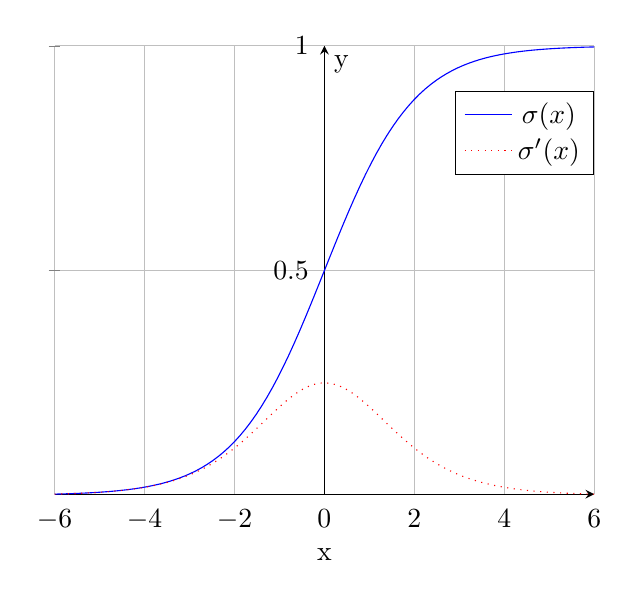
\begin{tikzpicture}[declare function={sigma(\x)=1/(1+exp(-\x));
    sigmap(\x)=sigma(\x)*(1-sigma(\x));}]
    \begin{axis}%
    [
        grid=major,     
        xmin=-6,
        xmax=6,
        axis x line=bottom,
        ytick={0,.5,1},
        ymax=1,
        ylabel= y,
        xlabel= x,
        ytick align=outside,
        ytick pos=left,
        major x tick style = transparent,
        axis y line=middle,
        samples=100,
        domain=-6:6,
        legend style={at={(1,0.9)}}     
    ]
        \addplot[blue,mark=none]   (x,{sigma(x)});
        \addplot[red,dotted,mark=none]   (x,{sigmap(x)});
        \legend{$\sigma(x)$,$\sigma'(x)$}
    \end{axis}
    \end{tikzpicture}
    
    \caption{Sigmoid function and its derivative.}
    \label{fig:sigmoid}
\end{figure}
Tranforming the data using sigmoid and then squazing it back between 0 and 1. 
Continous models can learn out-of-sample values. In this case it would be unphysical.

\subsection{Loss/ Metrics}  \label{sec:metrics}
In order to acquire a certain skill you need a measure determining how close you are. 
Use the sum of square or absolute values in order to not penalize point on the lower side of the line. Or not having to deal with negative distances. 
\begin{equation} \label{eq:mse}
    MSE(\hat{y},\hat{\tilde{y}}) = \frac{1}{n} \sum_{i=0}^{n-1}(y_i-\tilde{y}_i)^2
\end{equation} 

\begin{equation} \label{eq:ase}
    ASE(\hat{y},\hat{\tilde{y}}) =  \sum_{i=0}^{n-1}(y_i-\tilde{y}_i)^2
\end{equation} 

\begin{equation} \label{eq:r2}
    R^2(\hat{y}, \tilde{\hat{y}}) = 1 - \frac{\sum_{i=0}^{n - 1} (y_i - \tilde{y}_i)^2}{\sum_{i=0}^{n - 1} (y_i - \bar{y})^2}
\end{equation} 
where mean value of $\hat{y}$ is defined as $\bar{y} =  \frac{1}{n} \sum_{i=0}^{n - 1} y_i$. $R^2$ describes how much of the variation in the dataset you are able to capture with your model.

\subsection{Generalization} \label{sec:generalization}
% Move overfitting here
Finding a suitable curve for a set of points. Working with real data, noise is inevitable. In order to compensate, data is split into training and test (validation) sets. % better to call it something like generalization..?
Overall goal is to achieve the most general relation. \textit{For prediction purposes they can sometimes outperform fancier non-linear models, especially in situations with small numbers of training cases, low signal-to-noise ratio or sparse data.} \textbf{Hastie et al.} Overfitting becomes evident when you have a increase in the difference between the test- and training error. In non-mathematical terms, you have adjusted to much to the training data and where not able to find the general relation, program or "rules". See Figure \ref{fig:linreg_overfitting} 

\begin{figure}[hp]
    \centering
    \includegraphics[scale = 0.5]{Chapter3_Method/figs/generalization.png}
    \caption{Fitting at different levels. The optimal fit is the most general one. This is applicable to many cases. For the traditional autoregressive models, the predictor variable is the true value in the previous time step. \textbf{I'll make my own figure if we decide it should be a part of my thesis.}}
    \label{fig:linreg_overfitting}
\end{figure}

Its relevant for all ML algorithms but easiest to visualize for linear regression.
\textit{Overfitting a model is a condition where a statistical model begins to describe the random error in the data rather than the relationships between variables.}

\subsection{Automatic Optimization} \label{sec:hyperparam_tuning}
Keras-tuner. Tuning hyper-parameters.
\textit{A hyperparameter is a constant parameter whose value is set before the learning process begins.}

\textbf{Explain all the params you tune. Might be beneficially with a figure. See Rune's MS-thesis.}

\textit{Learning to forget found the best accuracy when using learning rate decay.}


Although theoretically fascinating it remains to see if LSTM provide a clear practical advantage over the autoregressive models.



\cleardoublepage

\chapter{Results and Discussion}
\section{Dataset - European Cloud Cover }
%This chapter presents the developed methodology used in the compilation of the dataset. 
This section presents the developed algorithms necessary for the compilation of the dataset \acrfull{ecc}. It is pieced together from two sources, ERA5 reanalysis and \acrlong{msg} cloud mask.

Several candidate satellites were studied before arriving at the combination of datasets presented in this chapter. Spatiotemporal consistency and resolution were given high priority. The variable cloud mask is provided by many satellites, bringing valuable information in itself, but also for the retrieval of other variables restricted to cloud free conditions, such as humidity. The satellite product chosen for this project is the \acrfull{msg}. This satellite is in geostationary orbit, and has an exceptional temporal resolution, scans every 15min. Knowing that the average lifetime of a cloud is 60min or less, it seems like a reasonable choice (\cite{lohmann2016}, pp. 19). The finished dataset, described in detail below, is named \acrfull{ecc}.

\subsection{Domain}
The geographical domain has, for this project, been restricted to latitude, $\theta \in[30,50]$ and longitude $\phi \in [-15, 25]$. The resulting dimensions of the grid become $81\times161$ pixels. Figure \ref{fig:map} shows the domain included in this dataset. The domain covers central Europe and north Africa.
\begin{figure}[h]
    \centering
    \includegraphics[scale = 1.0]{python_figs/Domain.png}
    \caption[Map over domain.]{Map showing the domain in the projection available in \acrshort{ecc}.}
    \label{fig:map}
\end{figure}

\subsection{Physical basis of variable decision} \label{sec:ecc}
The overall goal is to investigate whether basic meteorological variables such as temperature, pressure and humidity are sufficient for prediction of cloud fractional cover with a reasonable accuracy. Cloud dynamics is far more complicated than what can be describes by these variables, as discussed in Section \ref{sec:cloud_in_climate_system}.
%What is believed to be a sufficiently accurate model is further explained in Chapter \ref{ch:computer_experiments}.
The condition describing what is ``sufficiently accurate'' is further explained in Chapter \ref{ch:computer_experiments}.
%Reasonable accuracy can mean so much and it is different based on the method of evaluation and the chosen metric. A parametrization can be evaluated in isolation or in the context of a \acrshort{esm}-model. 
%There are several options when determining what is sufficiently accurate, a method can be evaluated in isolation and in the context of a climate model. In isolation it should be better than a a benchmark (chosen by ??) and in the context of a climate model it would be reducing the spread of uncertainty related to the variable we are predicting. 

This project is a \textit{proof of concept study} aimed to demonstrate the feasibility of using \acrshort{ai} to parametize \acrshort{cfc}. Employing data driven learning to represent cloud physics and dynamics in its full complexity requires measurements from technologies not yet invented. If they did exist, the computational cost would be enormous, and even then there would be no guarantee that the model performance would be %\textcolor{red}{the?} 
state-of-the-art.
%Not feasible in the foreseeable future to incorporate all the effects of micro-physics at a sufficient accuracy. 

Macrophysics properties describes the cloud as a unit, using properties like base height, top height, thickness, fractional cover and regime (also known as type). Microphysical processes are all mechanisms involving the particles forming a cloud. Examples of properties used to quantify the microphysical state
%\textcolor{red}{Synes "making up" a cloud hørtes litt rart ut, men det er du som er skyeksperten. Ville vurdert en annen beskrivelse hvis du har}. Examples of these variable \textcolor{red}{I setningen før har du kalt det for microphysical processes som er alle mechanisms. ville da også vurdert å bruke det videre "Examples of these mechanisms/microphysiacal processes are...." og evt. " and is treated as variables in the model/study" eller noe lignende} 
are \acrshort{ccn} and droplet number concentrations (\cite{Grabowski2019ModelingBetter}). Precipitation formation and cloud optical thickness are affected by changes on a microphysical level. However, they are undeniably closely related to the macrophysical properties of the cloud. Imagine precipitation without a cloud fractional cover? 

Reliable estimates of large-scale variables are available from using reanalyse or other climate models. Restricting the focus to the macrophysical aspect of clouds  makes it reasonable to chose these as explanatory variables and thereby ensuring that it is possible to build usable application of this parameterization in the future.

%Focusing on the macrophysical aspect of clouds its is reasonable to chose large-scale variables \textcolor{red}{Rar setning. gir ingen mening å bruke "its". Mener du kanskje "Focusing on the macro-physical aspect of clouds, it is reasonable to chose large-scale variables,..."}, for which reliable estimates are available from using reanalyse or other climate models, thereby ensuring that it is possible to build usable application of this in the future. \textcolor{red}{ALTFOR lang setning. Hele avsnittet er en setning! }
%\textcolor{red}{Focusing on the macro-physical aspect of clouds, it is reasonable to chose large-scale variables. Because, reliable estimates are available from the use of reanalyse or other climate models. It then ensures that it is possible to build usable application of this (hva er this? the variables?) in the future.}
For this dataset, all variables are produced by ERA5. Some variables have been chosen because they are reliable and fundamental meteorological variables, e.g. temperature and surface pressure. Others because they are essential in cloud formation, e.g. specific and relative humidity. They are all retrieved from the surface or the closest pressure level (1000hPa). The following section gives a brief introduction to their role in cloud formation. %\textcolor{red}{(Nå er du midt i seksjonen, så føles litt rart at du kommer med dette her, men kan kanskje heller si at "the rest of the section gives a brief ...."}

From the weather maps on the news, low and high pressure systems might be familiar terms. Low pressure systems are often associated with precipitation, while high pressure systems are associated with nice weather. The earth is not equally heated due to the earths spherical geometry. Warmer air rises, generating a low pressure at the surface. As the air rises the temperature decreases. From Equation \eqref{eq:clausius_clapeyron} it can be shown that, colder air can retain less vapour, enhancing the rate at which saturation is achieved. Under supersaturated conditions some of the vapour condenses, generating cloud water, forming a cloud, and occasionally precipitation. Summer is often associated with convective motions generating cumulus type clouds. %Evaporation rates 
%In presence of water at the surface, evaporation rates are also higher in a warmer climate \textcolor{red}{eller ikke? Fordamping drives vel av forskjellen i luftfuktighet ved bakken og luften i tillegg til vind? SElv om det er veldig varmt, men høy luftfuktighet så vil du ha lite fordamping. Så drivkraften er ikke varme. Tror ligningen er noe som fordamping = (e-es)*u hvor e er vannmetning i lufta og es ved overflaten eller noe og u er vind (men dette er tatt ut av hukommelsen og jeg ville sjekket det i Dingman)}. \textcolor{red}{Ellers et veldig bra avsnitt! Tydelig og enkelt forklart på en bra måte}

In areas of lower pressure, the surrounding air will flow toward the low pressure centre to offset the pressure difference. Induced by earths rotation the Coriolis effect force winds of low pressure system to swirl counterclockwise north of the equator and clockwise south of the equator, causing an accumulation of air in the centre of low pressure system. Pushing it to higher altitudes in the atmosphere. A high pressure system exhibit the exact opposite behaviour, it swirls in the reverse direction, and the air flows from the centre. Diverging air masses cause sinking motions of parcels from higher in the atmosphere to fill the void. 
% air from higher in the atmosphere to sink and fill the space left.
% \textit{Air from higher in the atmosphere sinks down to fill the space left as air moves outward.} 
Winds transports the substances suspended in air, such as pollutants and humidity. 

The dataset includes both relative and specific humidity. Relative humidity is a measure of how much vapour the air contains, relative to how much it can hold at a certain temperature. At relative humidity of 1 the air is at its dew point, and for higher values clouds form, under such supersaturated conditions it is often referred to as \textbf{X}, and therefore it is common to limit the range of relative humidity to be between 0 and 1. However the variable is still a measure of the identical ratio, and this explains why values exceeding 1 is present in the dataset. Relative humidity is unitless and for higher values the air is more humid.

Specific humidity is the ratio between mass of vapour and mass of air, with unit of $kg kg^{-1}$ (\cite{lohmann2016}, pp. 53-54). Whether relative or specific humidity is the better predictor is not clear a priori. The data is gathered from the model level closest to the surface, at an altitude of 1000hPa (\cite{lohmann2016}, pp. 81-84). \textbf{Les sidene igjen. Siteringen er nok på feil plass...}

\subsection{Area Weighting Regridding Scheme (AWRS)} \label{sec:remapping}
Computing cloud fractions based on cloud mask requires a regridding scheme. Common schemes for solving similar tasks are mean, nearest neighbour or area weighting. For this particular task, the pixels are of uneven size and the area weighted scheme seemed most appropriate. 

This section provides a step-by-step description of the necessary data processing done for the compilation of \acrshort{ecc}, transforming clouds masks provided in \textit{space-view} to cloud fractions on a uniform grid. \acrshort{eumetsat} doesn't provide suitable software to tackle this particular task (personal communication EUMETSAT staff). Building the dataset requires the implementations of software with functionality to perform the regridding, described in detail below, named the \acrfull{awrs}.

The regridding algorithm consist of two modules; \textit{(1) detection} and \textit{(2) area weighting algorithmn}. Let the subscripts denote the dataset pertaining to a particular grid. Grid\textsubscript{MSG} refers to the space-view grid of the \acrlong{msg} and grid\textsubscript{ECC} refers to the uniform grid originating from ERA5. Note that grid\textsubscript{ECC} is identical to  grid\textsubscript{ERA5}. The \textit{detection algorithmn}, determines the contributing pixel from grid\textsubscript{MSG} 
to the particular cells in the other coordinate system,
grid\textsubscript{ERA5} 
and their classification into the different categories such as \textit{corner}, \textit{centre}, \textit{left}, \textit{right}, \textit{upper} and \textit{lower boundary}. These categories are later used to isolate the portion of the pixel contributing to grid\textsubscript{ECC}.
%This is necessary to compute the area of the overlapping pixels. 
%\textbf{Include somewhere? In order to compute the area of the boundary pixels, their centre need to be rectified to the centre of the subsection that fall within the boundaries of grid\textsubscript{ECC}, and the pixel extent need to be updated.}
The second module, \textit{the area weighting}, consist of the category based area weighting algorithm based on the developed equations.

\subsubsection{Equations describing grid area}
Based on the assumptions  of a spherical earth the pixels areas are computed using spherical coordinates. Figure \ref{fig:spherical_coords} shows a square projected on to a sphere. Deriving the equation for computing the area of a square in spherical coordinates, requires integrating over changes in latitude, $d\theta$ and longitude, $d\phi$. In Equation \eqref{eq:sphere_integral} the variables of integration is given a prime to keep them distinct from the integration boundaries.
\begin{figure}
    \centering
    
    
\tdplotsetmaincoords{60}{110}
%
\pgfmathsetmacro{\rvec}{1.0}
\pgfmathsetmacro{\thetavec}{30}
\pgfmathsetmacro{\phivec}{60}

\pgfmathsetmacro{\deltathetavec}{40}
\pgfmathsetmacro{\deltaphivec}{80}

%
\begin{tikzpicture}[scale=5,tdplot_main_coords]
    \coordinate (O) at (0,0,0); % origo

    \coordinate (z) at (0, 0, 1.0); % origo
    %\draw[thin, <->] (1, 0.7, 1.16) -- (1, 0.52, 1.2) node[pos = 0.8, above right]{\Large $d\theta$};
    
    \draw[very thick,->] (0,0,0) -- (1.7, 0, 0) node[anchor=north east]{\Large $x$};
    \draw[very thick,->] (0,0,0) -- (0, 1.7, 0) node[anchor=north west]{\Large $y$};
    \draw[very thick,->] (0,0,0) -- (0, 0, 1.7) node[anchor=south]{\Large $z$};
    \shade[ball color = teal, opacity = 0.1] (0,0,0) circle [radius=\rvec];
    \draw (0,0,0) circle [radius=\rvec];
    
    \tdplotsetcoord{P}{\rvec}{\thetavec}{\phivec}
    \tdplotsetcoord{dP}{\rvec}{\deltathetavec}{\phivec}
    
    \tdplotsetcoord{G}{\rvec}{\thetavec}{\deltaphivec}
    \tdplotsetcoord{dG}{\rvec}{\deltathetavec}{\deltaphivec}

    \draw[very thick, color=teal, opacity = 0.3] (O) -- (G) node[above right]  {};
    \draw[very thick, color=teal, opacity = 0.6] (O) -- (dG) node[above right] {};    
    \draw[very thick, color=teal, opacity = 0.6] (O) -- (P) node[above right]  {};
    \draw[very thick, color=teal, opacity = 0.6] (O) -- (dP) node[above right] {};
    
    \draw[dashed, color=teal] (O) -- (Pxy);
    \draw[dashed, color=teal] (dP) -- (Pxy);
    %\draw[dashed, color=red] (Pz) -- (Py);


    %\draw[dashed, color=red] (dP) -- (Pxy);
    
    \draw[dashed, color=teal] (O) -- (Gxy);
    \draw[dashed, color=teal] (dG) -- (Gxy);
    \draw[dashed, color=black,looseness = 10, bend left] (z) -- (G)  node[pos = 0.6, above right] {\Large $rsin\theta$};
    \draw[dashed, color=teal,looseness = 10, bend left] (z) -- (G);
    \draw[dashed, color=teal, bend right] (P) -- (z);
    
    
    \draw [] (\phivec:0.5)  arc (\phivec:\deltaphivec:0.5) node [below right, pos=0.3] {\Large $d\phi$};

    
    %\tdplotdrawarc[tdplot_rotated_coords, ->]{(dP)}{.7}{(Pxy)}
    
    \draw[dashed, very thick, color=teal, fill = teal, opacity = 0.2] (P) -- (dP) -- (dG) -- (G) -- (P);
    \draw[dashed, very thick, color=teal] (P) -- (dP) -- (dG) -- (G) -- (P);
    \draw[dashed, color=black] (dG) -- (G) node[pos = 0.5, above right] {\Large $rd\theta$};
    \draw[dashed, color=teal] (dG) -- (G);    \tdplotdrawarc[]{(O)}{0.4}{0}{\phivec}{anchor=north}{\Large $\phi$}
    %\tdplotdrawarc{(O)}{0.2}{0}{\deltathetavec}{anchor=north}{$\theta$}

    \tdplotsetthetaplanecoords{\phivec};
    
    \tdplotdrawarc[tdplot_rotated_coords]{(0,0,0)}{0.8}{0}%
        {\thetavec}{anchor=south west}{\Large $\theta$};
    
    \tdplotdrawarc[tdplot_rotated_coords, pos = 0.5]{(0,0,0.2)}{0.26}{0}%
        {\thetavec}{anchor = south west,shift={(4mm,-5mm)}}{\Large $d\theta$};
        
    %\tdplotdrawarc[tdplot_rotated_coords, <->]{(0.1, 0.2, 0)}{.5}{0}{\thetavec}{anchor=east}{\Large $d\theta$}
    \shade[ball color=teal,tdplot_screen_coords,opacity=0.1] (O) circle[radius=\rvec];
    \foreach \X/\Y in {xy/z,yz/x,zx/y}
        {\begin{scope}[canvas is \X\space plane at \Y=\rvec]
         \fill circle[radius=1pt];
        \end{scope}}
    \end{tikzpicture}
    
    \caption{Map projection}
    \label{fig:spherical_coords}
\end{figure}
The general expression for the area of a square in spherical coordinates, is given by the following integral,
\begin{equation} \label{eq:sphere_integral}
    A = R^2\int_{ \theta - \delta \theta }^{\theta + \delta \theta} \int_{ \phi - \delta \phi }^{\phi + \delta \phi} cos\left( \theta' \right) d\phi' d\theta'
\end{equation}
%This can be rewriting into, \textbf{needs indices $(i, j)$ ..?}
the equation can be rewritten into,
\begin{equation} \label{eq:sphere_finish}
    A \left( \theta, \phi, \delta \theta, \delta \phi   \right)= 2R^2 \left( sin\left( \theta + \delta \theta  \right) - sin\left(  \theta - \delta \theta  \right) \right) \delta \phi
\end{equation}
where $R=6378km$ denotes the distance to earths centre, $\theta$ the latitude and $\phi$ the longitude. Relating Equations \eqref{eq:sphere_integral} and \eqref{eq:sphere_finish} to Figure \ref{fig:spherical_coords} by setting $d \theta = 2 \delta \theta$ and $d \phi = 2 \delta \phi$. The implementation is scaled by $R$.

The equations used to compute the area weighted cloud fractional cover is as follows,
\begin{equation} \label{eq:area_weighting}
    CFC_{ECC} = \frac{1}{A} \sum_{i=0}^{N} a_i m_i
\end{equation}
where,
\begin{equation} \label{eq:tot_area}
    A = \sum_{i=0}^{N} a_i
\end{equation}
Inserting $m_i = 1$ $\forall$ $i \in [0,N]$ into Equation \eqref{eq:area_weighting} results in $CFC_{ECC}=1$, independent of $a_i$, proving that the minor overlap between pixels in Figure \ref{fig:pixels_contributing_to_cell} doesn't affect the range of cloud fractions, which remains between 0 and 1.

\subsubsection{Estimating properties of grid\textsubscript{MSG}}
% Estimating the extent of the cell.
The coordinate information is provided in grids of latitudes, $\theta$ (degrees north), and longitudes, $\phi$ (degrees east) values. The coordinate represent the centre of a pixel. To acquire the information about the extent of cells in a non-uniform grid require some simplifications. 

%%%%%%%%%%%%% PART ONE
Computing the area weighted average of cloud masks requires detecting the grid\textsubscript{MSG}
contributing to the grid\textsubscript{ERA5} cell, and computing their area. The pixels are classified into five categories; \textit{centre}, \textit{left}, \textit{right}, \textit{up} and \textit{down boundary}.
%The detection algorithm is straight forward, overlapping pixels are included and labelled with a suitable category.
The cloud mask pixels are smallest at the nadir point, decreasing in all directions. Figure \ref{fig:estimate_dlon} illustrates this by showing an example of three neighbouring pixels. In this example the apparent pixel size increases going eastward. Consequently, there is an asymmetry between neighbouring pixels. The distance from the centre to the right and left neighbour is unequal. In order to take advantage of the analytical expression derived in Equation \eqref{eq:sphere_finish}, the extent of a contributing pixel is approximated by averaging the right and left distances. The categorisation is illustrated in Figure \ref{fig:pixels_contributing_to_cell} using different colours.

\tdplotsetmaincoords{60}{110}
%
\pgfmathsetmacro{\rvec}{1.6}
\pgfmathsetmacro{\thetavec}{30}
\pgfmathsetmacro{\phivec}{60}

\pgfmathsetmacro{\deltathetavec}{40}
\pgfmathsetmacro{\deltaphivec}{80}

\begin{figure}
    \centering
    
    
\tdplotsetmaincoords{60}{110}
%
\pgfmathsetmacro{\rvec}{1.0}

\pgfmathsetmacro{\thetavec}{30}
\pgfmathsetmacro{\deltathetavec}{40}
\pgfmathsetmacro{\deltatwothetavec}{50}
\pgfmathsetmacro{\deltathreethetavec}{60}

\pgfmathsetmacro{\phivec}{-30}
\pgfmathsetmacro{\deltaphivec}{10}
\pgfmathsetmacro{\deltatwophivec}{50}
\pgfmathsetmacro{\deltathreephivec}{90}



\begin{tikzpicture}[scale=5,tdplot_main_coords, 
                    mycirc/.style={circle,fill=blue!20, minimum size=0.5cm}]

    %%%%%%%%%%%%%% Setting up axis and coordinate system.
    \coordinate (O) at (0,0,0); % origo
    \coordinate (z) at (0, 0, \rvec); % origo
    %\draw[thin, <->] (1, 0.7, 1.16) -- (1, 0.52, 1.2) node[pos = 0.8, above right]{\Large $d\theta$};
    \draw[very thick,->, opacity = 1.] (0,0,0) -- (1.7, 0, 0) node[anchor=north east]{\Large $x$};
    \draw[very thick,->,  opacity = 1.] (0,0,0) -- (0, 1.7, 0) node[anchor=north west]{\Large $y$};
    \draw[very thick,->,  opacity = 1.] (0,0,0) -- (0, 0, 1.7) node[anchor=south]{\Large $z$};
    \shade[ball color = teal, opacity = 0.1] (0,0,0) circle [radius=\rvec];
    \draw (0,0,0) circle [radius=\rvec];

    
    \tdplotsetcoord{a}{\rvec}{\deltathetavec}{\phivec}
    \tdplotsetcoord{b}{\rvec}{\deltatwothetavec}{\phivec}
    % Changeing the rightmost part 
    \tdplotsetcoord{c}{\rvec}{\deltathetavec-5}{\deltaphivec}
    \tdplotsetcoord{d}{\rvec}{\deltatwothetavec+5}{\deltaphivec}
    
    \draw[dashed, very thick, color=teal, fill = teal, opacity = 0.2] (a) -- (b) -- (d)-- (c) -- (a);
    \draw[dashed, very thick, color=teal] (a) -- (b) -- (d)-- (c) -- (a);

    \tdplotsetcoord{a}{\rvec}{\deltathetavec-5}{\deltaphivec}
    \tdplotsetcoord{b}{\rvec}{\deltatwothetavec+5}{\deltaphivec}
    \tdplotsetcoord{c}{\rvec}{\deltathetavec-10}{\deltatwophivec}
    \tdplotsetcoord{d}{\rvec}{\deltatwothetavec+10}{\deltatwophivec}
    
    \draw[dashed, very thick, color=teal, fill = teal, opacity = 0.2] (a) -- (b) -- (d)-- (c) -- (a);
    \draw[dashed, very thick, color=teal] (a) -- (b) -- (d)-- (c) -- (a);
        
    % First column
    %\node[draw] at (0, -2)  (c)     {C};
    %\node[draw] at (0.3, -0.25, 0.5) {$\phi_{(i,j-1)}$};
    %\node[draw, thick] at (0.5, 0.3, 0.65) {$\phi_{(i,j)})$};
    %\node[draw, thick] at (0.5, 0.73, 0.87) {$(i,j+1)$};
    \filldraw [teal, label=above:{$\phi_{(i,j-1)}$}]  (0.3, -0.25, 0.5) circle (1pt);
    \filldraw [teal, label=above:{$\phi_{(i,j-1)}$}]  (0.5, 0.3, 0.65)  circle (1pt);
    \filldraw [teal, label=above:{$\phi_{(i,j-1)}$}]  (0.5, 0.73, 0.87) circle (1pt);
    
    \tdplotsetcoord{a}{\rvec}{\deltathetavec-10}{\deltatwophivec}
    \tdplotsetcoord{b}{\rvec}{\deltatwothetavec+10}{\deltatwophivec}
    \tdplotsetcoord{c}{\rvec}{\deltathetavec-15}{\deltathreephivec}
    \tdplotsetcoord{d}{\rvec}{\deltatwothetavec+15}{\deltathreephivec}
    
    \draw[dashed, very thick, color=teal, fill = teal, opacity = 0.2] (a) -- (b) -- (d)-- (c) -- (a);
    \draw[dashed, very thick, color=teal] (a) -- (b) -- (d)-- (c) -- (a);
    
    \draw [decorate,decoration={brace, amplitude=12pt, mirror}, xshift=0pt, yshift=0pt]
    (0.3, -0.25, 0.1) -- (0.5, 0.83, 0.47) node [black,midway,xshift=0.2cm, yshift = -1.5cm, very thick] {\Large $\left| \phi_{i+1,j} - \phi_{i-1, j} \right| $};
    
    \draw [decorate,decoration={brace, amplitude=12pt}, xshift=0pt, yshift=0pt]
    (0.5, 0.3, 0.65) -- ((0.5, 0.5, 0.73) node [black,midway,xshift=0cm, yshift = 2.cm, very thick] {\Large $\delta \phi_{(i, j)}$};

    \tdplotsetthetaplanecoords{\phivec};
    \shade[ball color=teal,tdplot_screen_coords,opacity=0.1] (O) circle[radius=\rvec];
    \foreach \X/\Y in {xy/z,yz/x,zx/y}
        {\begin{scope}[canvas is \X\space plane at \Y=\rvec]
         \fill circle[radius=1pt];
        \end{scope}}
    \end{tikzpicture}
    
    \caption{Illustrating the relative size of three neighbouring pixels on a sphere in the \textit{space-view} grid provided by EUMETSAT. The following example explain the changes in longitude, $\phi$, varying in eastward direction, denoted $i$. The expression is shown in Equation \eqref{eq:app_lon}. 
    The same principles applies in the latitudinal direction, see Equation \eqref{eq:app_lat}.  }
    \label{fig:estimate_dlon}
\end{figure}

\begin{figure}
    \centering
    \includegraphics{python_figs/example_remapping_lat45_lon25.pdf}
    \caption{Example showing the contributing pixels to the remapping of pixel $(25, 45)$. The pixels from the satellite is classified into corner (grey), centre (pink), right (purple), left (yellow), down (green) and up (blue) boundary. The dense black line is the pixel in grid\textsubscript{ECC}, and the other pixels shows the contributing pixels from grid\textsubscript{MSG}.}
    \label{fig:pixels_contributing_to_cell}
\end{figure}

Approximation of $d\phi$ and $d\theta$ have been done based on the two-dimensional fields of latitude and longitude values according to the below equations.
Longitudinal values vary along the first dimension, denoted with index i. The estimated half the extent of a pixel in grid\textsubscript{MSG} is approximated by Equation \eqref{eq:app_lon}. Latitudinal changes are in north-south direction, along the second-axis, here denoted with index, j. Equation \eqref{eq:app_lat} describes the distance from the centre to the upper and lower boundary.
% \eqref{eq:app_lon} and  \eqref{eq:app_lat}. 
%The horizontal extent of a pixel $(i,j)$ be determined by the the averaged distance between the longitude of neighbouring pixels. 
%, see Equation \eqref{eq:app_lon}. The same principles applies in the latitudinal direction, this version is shown in Equation \ref{eq:app_lat}.
\begin{equation} \label{eq:app_lon}
    \delta \phi_{i,j} = \left| \frac{\phi_{i+1,j} - \phi_{i-1, j}}{4} \right|
\end{equation}
\begin{equation} \label{eq:app_lat}
    \delta \theta_{i,j} = \left| \frac{\theta_{i,j+1} - \theta_{i, j-1}}{4} \right|
\end{equation}

The ``square'' in grid\textsubscript{MSG} resembles a trapezium, as illustrated in Figure \ref{fig:estimate_dlon}. As far as the author know, it doesn't exist an analytical solution to an area of a trapezium in spherical coordinates. Also, it is not clear if approximating the area with another numerical method would reduce the overall uncertainty. However, it would most likely increase the computational time. 
A visual inspection of the relation between both grids is provided in 
Figure \ref{fig:pixels_contributing_to_cell}. Based on the small overlapping areas, it appears to be a reasonable simplification at the latitudes and longitudes of interest. This particular pixel was chosen since the largest overlap is expected in the periphery of grid\textsubscript{ECC}. The inclusion of the boundary pixels involve estimating the ``new'' centre and the extent of the contributing portion. Defined as the subset falling within the boundaries of grid\textsubscript{ECC}. Due to the small overlap between contribution pixel, occasionally more than four pixels are classified as corners. For the sake of simplicity the corner pixels where omitted from the calculations of cloud fraction. This may have caused the circular pattern shown in Figure \ref{fig:area_pixel_signal}. The areas decrease poleward, as illustrated in Figure \ref{fig:relative_size_neigbouring_pixels}. This again have most likely enlarged the radius of the circular pattern.
\begin{figure}[ht]
    \centering
    \includegraphics{python_figs/signal_area_pixel.pdf}
    \caption{Pixel areas decreasing poleward, also the pattern appear to be more pronounced close to the meridian decreasing in both east and west direction.}
    \label{fig:area_pixel_signal}
\end{figure} 

\tdplotsetmaincoords{60}{110}
%
\pgfmathsetmacro{\rvec}{1.6}
\pgfmathsetmacro{\thetavec}{30}
\pgfmathsetmacro{\phivec}{60}

\pgfmathsetmacro{\deltathetavec}{40}
\pgfmathsetmacro{\deltaphivec}{80}

\begin{figure}
    \centering
    
    
\tdplotsetmaincoords{60}{110}
%
\pgfmathsetmacro{\rvec}{1.0}

\pgfmathsetmacro{\thetavec}{30}
\pgfmathsetmacro{\deltathetavec}{40}
\pgfmathsetmacro{\deltatwothetavec}{50}
\pgfmathsetmacro{\deltathreethetavec}{60}

\pgfmathsetmacro{\phivec}{-30}
\pgfmathsetmacro{\deltaphivec}{10}
\pgfmathsetmacro{\deltatwophivec}{50}
\pgfmathsetmacro{\deltathreephivec}{90}

\begin{tikzpicture}[scale=5,tdplot_main_coords]

    %%%%%%%%%%%%%% Setting up axis and coordinate system.
    \coordinate (O) at (0,0,0); % origo
    \coordinate (z) at (0, 0, \rvec); % origo
    %\draw[thin, <->] (1, 0.7, 1.16) -- (1, 0.52, 1.2) node[pos = 0.8, above right]{\Large $d\theta$};
    \draw[very thick,->, opacity = 1.] (0,0,0) -- (1.7, 0, 0) node[anchor=north east]{\Large $x$};
    \draw[very thick,->,  opacity = 1.] (0,0,0) -- (0, 1.7, 0) node[anchor=north west]{\Large $y$};
    \draw[very thick,->,  opacity = 1.] (0,0,0) -- (0, 0, 1.7) node[anchor=south]{\Large $z$};
    \shade[ball color = teal, opacity = 0.1] (0,0,0) circle [radius=\rvec];
    \draw (0,0,0) circle [radius=\rvec];

    %%%%%%%%%%%%%%%%%%%%%%%%%%%% first column
    \tdplotsetcoord{P}{\rvec}{\thetavec}{\phivec}
    \tdplotsetcoord{dP}{\rvec}{\deltathetavec}{\phivec}
    \tdplotsetcoord{G}{\rvec}{\thetavec}{\deltaphivec}
    \tdplotsetcoord{dG}{\rvec}{\deltathetavec}{\deltaphivec}
    
    \draw[dashed, very thick, color=teal, fill = teal, opacity = 0.2] (P) -- (dP) -- (dG) -- (G) -- (P);
    \draw[dashed, very thick, color=teal] (P) -- (dP) -- (dG) -- (G) -- (P);
    
    \tdplotsetcoord{a}{\rvec}{\deltathetavec}{\phivec}
    \tdplotsetcoord{b}{\rvec}{\deltatwothetavec}{\phivec}
    \tdplotsetcoord{c}{\rvec}{\deltathetavec}{\deltaphivec}
    \tdplotsetcoord{d}{\rvec}{\deltatwothetavec}{\deltaphivec}
    
    \draw[dashed, very thick, color=teal, fill = teal, opacity = 0.2] (a) -- (b) -- (d)-- (c) -- (a);
    \draw[dashed, very thick, color=teal] (a) -- (b) -- (d)-- (c) -- (a);
    
    \tdplotsetcoord{e}{\rvec}{\deltatwothetavec}{\phivec}
    \tdplotsetcoord{f}{\rvec}{\deltathreethetavec}{\phivec}
    \tdplotsetcoord{g}{\rvec}{\deltatwothetavec}{\deltaphivec}
    \tdplotsetcoord{h}{\rvec}{\deltathreethetavec}{\deltaphivec}
    
    \draw[dashed, very thick, color=teal, fill = teal, opacity = 0.2] (e) -- (f) -- (h)-- (g) -- (e);
    \draw[dashed, very thick, color=teal] (e) -- (f) -- (h)-- (g) -- (e);

    %%%%%%%%%%%%%%%%%%%%%%%%%%%%%%%% second column
      
    \tdplotsetcoord{P}{\rvec}{\thetavec}{\deltaphivec}
    \tdplotsetcoord{dP}{\rvec}{\deltathetavec}{\deltaphivec}
    \tdplotsetcoord{G}{\rvec}{\thetavec}{\deltatwophivec}
    \tdplotsetcoord{dG}{\rvec}{\deltathetavec}{\deltatwophivec}
    
    \draw[dashed, very thick, color=teal, fill = teal, opacity = 0.2] (P) -- (dP) -- (dG) -- (G) -- (P);
    \draw[dashed, very thick, color=teal] (P) -- (dP) -- (dG) -- (G) -- (P);
  
      
    \tdplotsetcoord{a}{\rvec}{\deltathetavec}{\deltaphivec}
    \tdplotsetcoord{b}{\rvec}{\deltatwothetavec}{\deltaphivec}
    \tdplotsetcoord{c}{\rvec}{\deltathetavec}{\deltatwophivec}
    \tdplotsetcoord{d}{\rvec}{\deltatwothetavec}{\deltatwophivec}
    
    \draw[dashed, very thick, color=teal, fill = teal, opacity = 0.2] (a) -- (b) -- (d)-- (c) -- (a);
    \draw[dashed, very thick, color=teal] (a) -- (b) -- (d)-- (c) -- (a);
  
  
    \tdplotsetcoord{e}{\rvec}{\deltatwothetavec}{\deltaphivec}
    \tdplotsetcoord{f}{\rvec}{\deltathreethetavec}{\deltaphivec}
    \tdplotsetcoord{g}{\rvec}{\deltatwothetavec}{\deltatwophivec}
    \tdplotsetcoord{h}{\rvec}{\deltathreethetavec}{\deltatwophivec}
    
    \draw[dashed, very thick, color=teal, fill = teal, opacity = 0.2] (e) -- (f) -- (h)-- (g) -- (e);
    \draw[dashed, very thick, color=teal] (e) -- (f) -- (h)-- (g) -- (e);
    
    
    %%%%%%%%%%%%%%%%%%%%%%%%%%%%%%%% third column
    \tdplotsetcoord{P}{\rvec}{\thetavec}{\deltatwophivec}
    \tdplotsetcoord{dP}{\rvec}{\deltathetavec}{\deltatwophivec}
    \tdplotsetcoord{G}{\rvec}{\thetavec}{\deltathreephivec}
    \tdplotsetcoord{dG}{\rvec}{\deltathetavec}{\deltathreephivec}
    
    \draw[dashed, very thick, color=teal, fill = teal, opacity = 0.2] (P) -- (dP) -- (dG) -- (G) -- (P);
    \draw[dashed, very thick, color=teal] (P) -- (dP) -- (dG) -- (G) -- (P);
  
    \tdplotsetcoord{a}{\rvec}{\deltathetavec}{\deltatwophivec}
    \tdplotsetcoord{b}{\rvec}{\deltatwothetavec}{\deltatwophivec}
    \tdplotsetcoord{c}{\rvec}{\deltathetavec}{\deltathreephivec}
    \tdplotsetcoord{d}{\rvec}{\deltatwothetavec}{\deltathreephivec}
    
    \draw[dashed, very thick, color=teal, fill = teal, opacity = 0.2] (a) -- (b) -- (d)-- (c) -- (a);
    \draw[dashed, very thick, color=teal] (a) -- (b) -- (d)-- (c) -- (a);
  
    \tdplotsetcoord{e}{\rvec}{\deltatwothetavec}{\deltatwophivec}
    \tdplotsetcoord{f}{\rvec}{\deltathreethetavec}{\deltatwophivec}
    \tdplotsetcoord{g}{\rvec}{\deltatwothetavec}{\deltathreephivec}
    \tdplotsetcoord{h}{\rvec}{\deltathreethetavec}{\deltathreephivec}
    
    \draw[dashed, very thick, color=teal, fill = teal, opacity = 0.2] (e) -- (f) -- (h)-- (g) -- (e);
    \draw[dashed, very thick, color=teal] (e) -- (f) -- (h)-- (g) -- (e);
    
    %%%%%%%%%%%%%%%%%%%%%%%%%% Adding coordinate information

    % First column
    \draw[thick](0.3, -0.25, 0.5)node[scale=0.8, rotate = -15]{$(i,j-1)$};
    \draw[thick](0.3, -0.17, 0.7)node[scale=0.8, rotate = -15]{$(i+1,j-1)$};
    \draw[thick](0.3, -0.3, 0.3)node[scale=0.8, rotate = -15]{$(i-1,j-1)$};

    % Second column
    \draw[thick](0.5, 0.3, 0.65)node[scale=0.8, rotate = 5]{$(i,j)$};
    \draw[thick](0.5, 0.3, 0.85)node[scale=0.8, rotate = 5]{$(i+1,j)$};
    \draw[thick](0.5, 0.3, 0.45)node[scale=0.8, rotate = 5]{$(i-1,j)$};
    
    % Third column
    \draw[thick](0.5, 0.73, 0.87)node[scale=0.8, rotate = 35]{$(i,j+1)$};
    \draw[thick](0.5, 0.8, 0.7)node[scale=0.8, rotate = 35]{$(i-1,j+1)$};

    \draw[thick](0.05, 0.45, 0.73)node[scale=0.8, rotate = 35]{$(i+1,j+1)$};


    %\draw[dashed, color=teal] (dG) -- (G); 
    
    %\draw[very thick, color=teal, opacity = 0.3] (O) -- (G) node[above right]  {};
    %\draw[very thick, color=teal, opacity = 0.6] (O) -- (dG) node[above right] {};    
    %\draw[very thick, color=teal, opacity = 0.6] (O) -- (P) node[above right]  {};
    %\draw[very thick, color=teal, opacity = 0.6] (O) -- (dP) node[above right] {};
    
    %\draw[dashed, color=teal] (O) -- (Pxy);
    %\draw[dashed, color=teal] (dP) -- (Pxy);
    %\draw[dashed, color=red] (Pz) -- (Py);


    %\draw[dashed, color=red] (dP) -- (Pxy);
    
    %\draw[dashed, color=teal] (O) -- (Gxy);
    %\draw[dashed, color=teal] (dG) -- (Gxy);
    %\draw[dashed, color=black,looseness = 10, bend left] (z) -- (G)  node[pos = 0.6, above right] {\Large $rsin\theta$};
    %\draw[dashed, color=teal,looseness = 10, bend left] (z) -- (G);
    %\draw[dashed, color=teal, bend right] (P) -- (z);
    
    %\draw [] (\phivec:0.5)  arc (\phivec:\deltaphivec:0.5) node [below right, pos=0.3] {\Large $d\phi$};

    %\tdplotdrawarc[tdplot_rotated_coords, ->]{(dP)}{.7}{(Pxy)}

    %\draw[dashed, color=black] (dG) -- (G) node[pos = 0.5, above right] {\Large $rd\theta$};
   %\tdplotdrawarc[]{(O)}{0.4}{0}{\phivec}{anchor=north}{\Large $\phi$}
    %\tdplotdrawarc{(O)}{0.2}{0}{\deltathetavec}{anchor=north}{$\theta$}

    %\tdplotdrawarc[tdplot_rotated_coords]{(0,0,0)}{0.8}{0}%
    %    {\thetavec}{anchor=south west}{\Large $\theta$};
    
    %\tdplotdrawarc[tdplot_rotated_coords, pos = 0.5]{(0,0,0.2)}{0.26}{0}%
    %    {\thetavec}{anchor = south west,shift={(4mm,-5mm)}}{\Large $d\theta$};
        
    %\tdplotdrawarc[tdplot_rotated_coords, <->]{(0.1, 0.2, 0)}{.5}{0}{\thetavec}{anchor=east}{\Large $d\theta$}
    
    \tdplotsetthetaplanecoords{\phivec};
    \shade[ball color=teal,tdplot_screen_coords,opacity=0.1] (O) circle[radius=\rvec];
    \foreach \X/\Y in {xy/z,yz/x,zx/y}
        {\begin{scope}[canvas is \X\space plane at \Y=\rvec]
         \fill circle[radius=1pt];
        \end{scope}}
    \end{tikzpicture}
    
    \caption{Estimating the changes in latitude and longitude}
    \label{fig:estimate_dlat_dlon}
\end{figure}

\subsection{Verification of AWRS}
The regridding scheme is a set of algorithms. Before the production of the full dataset it is important verify the correctness the algorithms of \acrshort{awrs}.

%%%%%%%%%%%%%%%%%%%%%% TEST 1 - Formula to compute the area 
The computations of the areas are the foundation of the \acrshort{awrs}, and it it crucial to verify that the algorithm is correct. CDO (\cite{cdo}) provide functionality to compute gridarea of a uniform grid using the code inserted below.
\begin{verbatim}
$ cdo gridarea era5data.nc gridarea.nc     
\end{verbatim}
To verify the implementations of Equation \eqref{eq:sphere_finish}, the grid areas of ERA5 is computed using both CDO and the self implemented algorithm. Both versions produce the same results.
% må jeg skrive hvor like 
Emphazising that the self implemented code is scaled by $R$ to be consistent CDO. Multiplication followed by division of the same number provides no additional information, and there is the off chance of introducing additional numerical errors. 

%%%%%%%%%%%%%%%%% TEST 2 -- vis regridding
A reason of confusion in the process of developing the algorithm of the \acrshort{awrs} algorithm arose from the different rotations of the data provided by the \acrshort{grib} and \acrshort{netcdf} files. The coordinate information is availble in \acrshort{netcdf}, but the file-size is to large to store all data in this format, therefore the data is downloaded in \acrshort{grib}, as mention in Section \ref{sec:EUMETSAT_cloud_mask}. The \acrshort{grib}-file is provided as the left and right flipped version of the  \acrshort{netcdf}-file. A fast modular test to check the regridding routine is to insert the raw data including the land and sea masks. Figure \ref{fig:visual_inspection_regridding} shows a example of the regridding of the raw data from 2\textsuperscript{nd} May 2009. Clouds are illustrated in white, land mask in teal and ocean in purple. The original data also include the category off-earth disk, this is not a member of the chosen subset. By regridded the raw data it quickly becomes apparent whether correct domain has been used, and evident if the algorithm generates any discontinuities in space. 
\begin{figure}
    \centering
    \includegraphics{python_figs/visual_regridding.pdf}
    \caption{Result from regridding raw data, provided with land and sea masks in the absence of clouds. Land is illustrated in teal, ocean in purple and clouds in white.}
    \label{fig:visual_inspection_regridding}
\end{figure}

\subsection{Missing Data} \label{sec:missing_values}
Missing values is inevitable when working with observational data. Sensors fail to collect measurements and data is missing. This can either be individual pixels or entire disks. In this project single NaN values are no pressing issue since they are remapped to fractions by using the area weighted of the other values. Contributing NaN pixels are counted and stored for future use in \acrshort{ecc}.
\begin{figure}
    \centering
    \includegraphics[scale = 1.0]{python_figs/heatmap_missing_values.pdf}
    \caption{Heatmap summarising missing hours per month for all years.}
    \label{fig:heatmap_missing_values}
\end{figure}
\begin{figure}
    \centering
    \includegraphics[scale = 1.0]{python_figs/heatmap_missing_values_monthly_sum.pdf}
    \caption{Barplot showing the monthly sum of missing values. This excludes the contribution from the period of 2004 before the satellite was operational.}
    \label{fig:barplot_missing_values}
\end{figure}
In some cases the sensor fail to scan and in other cases the data has been destroyed prior to archiving. Independant of the cause, the result is the same, the data can never be recovered. %Further down the chain of supply, the missing data can cause issues for the process of downloading. Consequently, the requested data has entered infinity loop without being detected by \acrshort{eumetsat}. In combination with 
The maximum limit of pending request restricted to 20 have caused some delay. The data in each request amount to approximately 3.5 months of hourly data. 

Missing timestamps results in missing disks. When available the closest time step within the previous and trailing 45 minutes is used to fill the gap. A summary of missing values per month in the data set is provided in Figure \ref{fig:heatmap_missing_values}. Aggregation of missing values per month is presented in Figure \ref{fig:barplot_missing_values}. The plot is ment to illustrate any seasonal biases. The months of 2004 prior to the operalization of the satellite is not included as missing values.

METeosat provide a two satellite system, occasionally both standby and the operational scan at the same time, as mentioned in Section \ref{sec:meteosat}.
%To reduce the perturbations due to parallax (see Section X) of cloud, given a choice the operational satellite is chosen \textcolor{red}{(skjønte ikke setningen)}. 
In cases of technical failures, the standby scan is used. The scans are done from a different nominal position. However, the coordinate systems remain the same, since the standby scan is rectified to the position of the operational satellite before the product is released (personal communication \acrshort{eumetsat} staff). Comparing simultaneous measurements for the operational and the standby METeosat satellites, it becomes clear that they are disimilar. However, this doesn't occur to frequently and there has been no effort in quantifying the magnitude of the parallax, to correcting for for the bias it may introduce.
% again you have no numbers on the times the standby satellite is used.... 

Manually generated datasets are prone to human error, especially in the case where user need to download individual time steps to fill the gaps. The missing values was were double checked, but there is no guarantee that a few additional time steps is available. In summary the workflow has been as follows, the author downloaded the data, detect missing times and manually choose the closest time step available within the previous and trailing 45 minutes. In retrospect the, the downloading options (API or GUI) provided by the satellite service should be taken into account when choosing the data. A great API can potentially be a large time saver.

\subsection{Masks} \label{sec:mask}
The land sea masks are regridded from the HTAP-masks provided by \acrfull{metno}. In its original format the HTAP masks have a $0.1^o$ resolution and global coverage, not including the polar regions. These are regridded to a suitable resolution of $0.25^o$ using functionality available in PyAEROCOM (\cite{pyaerocom}). %(\href{https://pyaerocom.met.no/}{https://pyaerocom.met.no/}). 
This is a python toolbox developed within the \acrfull{aerocom} project. To avoid storing redundant data, only domain specific data is made available in the project supplementary repository. For more details on supplementary material, see Section \ref{sec:structure_and_implementations}.
%To keep memory-requirements to a minimum only the parts of the filters relevant domain is stored in the supplementary material for this project.
\begin{figure}
    \centering
    \includegraphics{python_figs/filters.pdf}
    \caption{Figure shows all filters, in white, available in the python package ``sciclouds''.}
    \label{fig:filters_subplot}
\end{figure}

Filters available in the supplementary material are \textit{land}, \textit{sea}, \textit{coastline} and \textit{artefact}. The coastline is defined to be all pixels that are not either 100\% land or sea. A threshold based binary classification is used to separate the coastline pixels into land or ocean. The threshold is set to 50\%. Pixels containing at least 50\% of sea is most likely affected by maritime conditions, making it reasonable to classify them as sea pixels.
\begin{figure}
    \centering
    \includegraphics{python_figs/example_artefact.pdf}
    \caption[Artefact in European Cloud Cover dataset.]{The results after regridding revels a artefact. This is a snapshot from May the second 2004 at noon. The frequency of occurrence is currently unknown.}
    \label{fig:example_artefact}
\end{figure}
Based on a visual comparison to Figure \ref{fig:example_artefact}, the artefact is defined to be all coastline pixels obeying the following inequality,  %\eqref{eq:artefact_condition}.
\begin{equation} \label{eq:artefact_condition}
    \theta + \frac{1}{3}\phi < 40
\end{equation}
All filters are displayed in Figure \ref{fig:filters_subplot}. 
%shows a subplot of all filters, including the artefact detecting filter. 
The signal form the artefact filter when applied to \acrshort{ecc} seem to follow a normal distribution as shown Figure \ref{fig:signal_artefact}. To get an idea of the frequency of appearance, it is necessary to detect when it appears in isolation and not in cloud. It could, for instance, be done by studying the histograms from the ratio of the artefact signal and a buffered artefact filter.
% Different approaches for detecting the artefact, separating the land, sea and coastline pixels. Filters to remove artefact in future. Can also use this compute statistics over land and ocean. Add land sea mask as subplot. 
No efforts have been made to remove the artefact from the data. %It is a thesis in itself %to remove the artefact 
%without introducing other complications like gaps in the dataset and or removing parts of an actual cloud.\textcolor{red}{Tenker det er unødvendig å ta med.... De skjønner at du har gjort mye jobb og at det er mye du kunne gjort, men ved å fortelle dem hvor mye jobb det er ved ulike oppgaver er ikke din oppgave her. Hold deg til problemstillingen din. }

\subsection{Statistical Properties in ECC}
To summarise and present the content of \acrshort{ecc} statistical properties are used. For clarity, the period used in this section is 2004 to 2018. The properties selected in this study is mean, minimum (min), maximum (max), median, \acrfull{std} and \acrfull{mad}. The most important results is presented in this section, and complementary figures can be found in the Appendix \ref{ch:appendix_statistic}. 
The data varies in space an time. Statistical properties are calculated over one or both these axis. %Determines the dimensions of the results. 
%\textbf{ Computing the statistical properties over one dimension, for instance time, leaves the spatial distribution of this property. Computing the statistics over space, leaves the temporal dimension. Computing the statistics over space and time leaves one value.} 

\subsubsection{Statistics over space and time}
%%% BAR PLOT GLOBAL STATISTICS
To study the statistical properties at different parts of the domain the filters, shown in Figure \ref{fig:filters_subplot}, were applied to the data before computing the statistical properties. Figure \ref{fig:bar_plot_global_stats} shows a barplot summarising the statistical properties for the five variables (Temperature, Surface Pressure, Cloud fractional cover, Specific and Relative humidity) and four filters (coast, land, sea and all). It shows minor differences between the statistical properties applied. The largest difference can be seen in the maximum value of relative humidity, where the maximum above land are larger than compared to ocean. The relative difference in magnitude between \acrshort{mad} and \acrshort{std} and the other variables from the reanalysis dataset, is solid. Most likely because the data is smoothed as a consequence of using assimilation model. 
\begin{figure}[ht]
    \centering
    \includegraphics{python_figs/bar_plot_global_statistics_new_legend.pdf}
    \caption{Bar plot showing global statistics for different filters.}
    \label{fig:bar_plot_global_stats}
\end{figure}

\subsubsection{Temporal statistics}
%%%%%%%%%%%%%%%%%%%%%%%%%%%%%%%%%%% MONTHLY MEANS
Figure \ref{fig:monthly_mean_ts_vars} shows the spatially averaged monthly mean values for all values. Seasonal effects and differences between land and ocean is evident among all variables. For temperature and relative humidity, a more pronounced seasonal cycle over land, compared to ocean, is evident. The remaining variables appear to have a small shift towards higher values.
\begin{figure}[ht]
    \centering
    \includegraphics{python_figs/monthly_means.pdf}
    \caption{Spatially averaged monthly values. Filters are applied for land and sea.}
    \label{fig:monthly_mean_ts_vars}
\end{figure}

The spatially averaged time series for the first week of August in 2012 is shown in Figure \ref{fig:first_week_august_2012}. Illustrating the relative strength of the signal feed to the input sequence. As a reference, the signal over land and ocean is provided. All variables display diurnal variations. Because of the different intervals of the axes, the magnitude of the signal proves difficult to determine from such a plot. The surface pressure over land and ocean appear to be a scaling of the ``no filter''. A common factor for all variables is the position if the filters relevant to each other, ``sea'' > ``no filter'' > ``land''. In some cases the monthly average temperature over land is higher than over ocean.
%Surface pressure provide nearly constant values and doesn't appear to be a good predictor. If a model predicting the same value as the day before, it doesn't provide more information. \textcolor{red}{En model kan vel gi samme informasjon som dagen før så lenge observasjonene ikke endrer seg. Ser ikke ut som cloud fractional cover helle rikke endrer seg så mye eller temperaturen. Temperaturen endrer seg bare med ca. 5 grader og det er vel ikke spesielt mye? Men du vet best, ville bare reagert på at det kan være aksene som gjør at det ser ut som en stor forskjell uten at det nødvendigvis er det. }
\begin{figure}[ht]
    \centering
    \includegraphics{python_figs/spatially_averaged_one_week_from_2012-08-01.png}
    \caption{Spatially averaged time series from the first week of August 2012.}
    \label{fig:first_week_august_2012}
\end{figure}


\subsubsection{Temporal statistics}
All the statistical properties computed over time for the variable \acrshort{cfc} in \acrshort{ecc} is plotted in 
Figure \ref{fig:all_stats_tcc}. Similar figures for the remaining variables in the dataset is presented in Section \ref{sec:all_stats}. %in the Appendix \ref{ch:appendix_statistic}. 
With the exception of minimum and maximum value, the cloud cover is affect by the coastline. 
%% CLOUD FRACTIONAL COVER
\begin{figure}[ht]
    \centering
    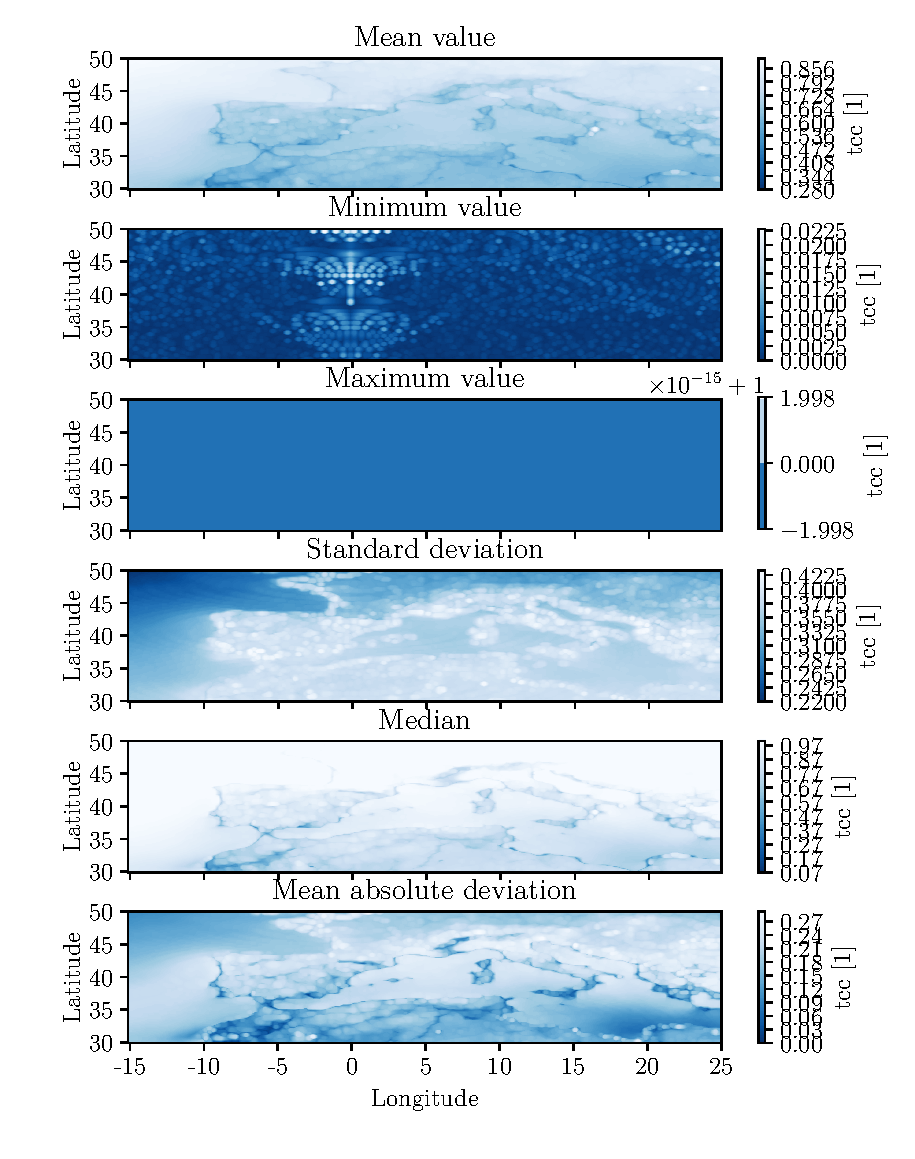
\includegraphics{python_figs/all_stat_variable_tcc.pdf}
    \caption{Contour plot showing the local (pixel) statistics for cloud fractional cover.}
    \label{fig:all_stats_tcc}
\end{figure}

The mean values displayed in figure \ref{fig:all_stats_tcc}, show that on average the coastline have a lower cloud cover than the adjacent areas. This is supported by the bar plot, see Figure \ref{fig:bar_plot_global_stats}. 

From the minimum values of \acrshort{cfc} it becomes evident that there is another artefact present in the dataset. This pattern is most likely caused by the remapping routine. Figure \ref{fig:area_pixel_signal} shows the patterns of magnitude of the areas contributing to a pixel. One might expect all pixels to be without cloud cover for at least on hour over the period of 14 years, but this is not the case. The maximum value is as expected, one over the entire region, indicating that at some point every pixel is full of clouds. The standard deviation is higher over land, this is caused by larger variation in cloud cover in these regions. The median and \acrshort{mad} 
% Det er jo ikke rart for mad er medianen av en differanse.
show similar patterns, this is not suprising since \acrshort{mad} is short for \acrlong{mad}, where the lowest values are found along the coast.

\subsubsection{Correlation between cloud cover and environmental variables}
%%% CORRELATION
Correlation describes how strong a pair of variables are linearly related. A positive correlation tells you that an increase in one variable results in an increase in the other. A negative correlation describes the opposite connection, implying that an increase in one variable cause a decrease in the other.
\begin{figure}[ht]
    \centering
    \includegraphics{python_figs/correlation_figure.pdf}
    \caption{Contour plot showing the correlation coefficient between environmental variables and cloud fractional cover.}
    \label{fig:correlation_tcc_vs_envio}
\end{figure}

The linear correlation coefficient from pairs of cloud cover and environmental variables such as temperature, pressure, relative and specific humidity is shown in Figure \ref{fig:correlation_tcc_vs_envio}. Recall that all environmental variables is produced by reanalysis. Pink illustrates negative correlation while green illustrates a positive correlation. Note that different patterns emerge from all variables. %, implying that they could be useful as predictors. 

Over land relative humidity is dominated by positive correlation to cloud cover, some part of Africa and the ocean in eastern Mediterranean has a negative correlation. The image of the surface pressure is remarkable similar, they share a pattern, but have opposite signs. The negative sign seems reasonable, since high pressure is often caused by sinking motions in the atmosphere and clouds are formed by rising motions. 

Specific humidity shows a clear shift at longitudinal degree 10. The land area in the west are positively correlated while the eastern part are  negatively correlated. 

In most locations temperature is negatively correlated with cloud cover except in parts of the Alps, north coast of France and in north Africa. This seems reasonable since warmer air can retain more vapours.%, on the other hand this could enhance evaporation rate, making more vapour available for condensing onto particles. 

% Finished regriddidng files.
\subsection{Summary}
\acrshort{ecc} comprises of five variables; temperature, pressure, cloud fractional cover, relative and specific humidity. These are collected from two sources; ERA5 and EUMETSAT. The resolution available in ERA5 was preserved, while remapping the cloud mask to cloud fractions cover. 
% duplication
The final product consist of %the variables temperature, pressure, cloud fraction, specific humidity and relative humidity, available
hourly data on a $0.25^o$ uniform grid resolution in the period from April 2004 to December 2018. Cloud fractional cover (\acrshort{cfc}) is produced from area weighting cloud masks. The \acrshort{awrs} is described in Section \ref{sec:remapping}. The remaining variables are on their original format as provided by \acrfull{ecmwf}. A summary of the original sources of the dataset is given in Table \ref{tab:dataset_summary}. More details on ERA5 is available in Section \ref{sec:era5} and for the cloud mask in Section \ref{sec:EUMETSAT_cloud_mask}. 
\begin{table}[ht]
    \centering
    \resizebox{\textwidth}{!}{%
\begin{tabular}{c|c|c|c|c|}
\cline{2-5}
\multirow{4}{*}{}                                 & \multicolumn{2}{c|}{\textbf{ERA5}}                                                                                                   & \multicolumn{2}{c|}{\textbf{MSG}}                                                                                                                \\ \cline{2-5} 
                                                  & \textbf{Type}                     & \textbf{Variables}                                                                               & \textbf{Type}                                                               & \textbf{Variables}                                                  \\ \cline{2-5} 
                                                  & Surface                           & \begin{tabular}[c]{@{}c@{}}2m Temperature\\ Surface pressure\end{tabular}                        & \multirow{2}{*}{Satelite retrival}                                          & \multirow{2}{*}{Cloud Mask}                                         \\ \cline{2-3}
                                                  & 1000 hPa                          & \begin{tabular}[c]{@{}c@{}}Relative Humidity\\ Specific Humidity\end{tabular}                    &                                                                             &                                                                     \\ \hline
\multicolumn{1}{|c|}{\textbf{Projection}}         & \multicolumn{2}{c|}{Uniform grid}                                                                                                    & \multicolumn{2}{c|}{Space-view grid}                                                                                                            \\ \hline
\multicolumn{1}{|l|}{\textbf{Spatial resolution}} & \multicolumn{2}{c|}{$0.25^o$}                                                                                                        & \multicolumn{2}{c|}{-}                                                                                                                            \\ \hline
\multicolumn{1}{|c|}{\textbf{Output Frequencey}}  & \multicolumn{2}{c|}{Hourly}                                                                                                          & \multicolumn{2}{c|}{15 min}                                                                                                                       \\ \hline
\multicolumn{1}{|c|}{\textbf{Availability}}       & \multicolumn{2}{c|}{\begin{tabular}[c]{@{}c@{}}1979-onwards\\ Expected to be available from \\ 1950 some time in 2020.\end{tabular}} & \multicolumn{2}{c|}{2004-onward}                                                                                                                 \\ \hline
\multicolumn{1}{|c|}{\textbf{License}}           & \multicolumn{2}{c|}{\begin{tabular}[c]{@{}c@{}}Open Access. Need user \\ from Copernicus Data Storage.\end{tabular}}                  & \multicolumn{2}{c|}{\begin{tabular}[c]{@{}c@{}}Researcher Licences\\ to get 15min resolution.\\ Open access (need user) \\  at hourly resolution\end{tabular}} \\ \hline
\end{tabular}
}
\caption{Summary of data used to compile \acrshort{ecc}.}
\label{tab:dataset_summary}
\end{table}
%Fractional cloud cover is computed from the cloud mask product retrieved by the second generations METeosat satellites. You can read more about this data in section \ref{sec:meteosat}. For simplicity we will refer to this dataset as European Cloud Cover Dataset, ECC from now on. The visual comparison between raw satellite images and cloud amount seem to agree. The cloud fractional distribution also retain the same shape as ERA5 and MODIS 6.1 Terra in the period from 2004 to 2018. \textbf{kilde?}

%\textbf{Something is missing here -- a table?}

%\subsection{Licences and Downloading Data} \label{sec:downloading_data}
%Scripts for downloading the ERA5 data used in this thesis is available in the project GitHub on \href{https://github.com/hannasv/MS/tree/metos/downloading{\_}RA}{https://github.com/hannasv/MS/tree/metos/downloading{\_}RA}. However you will need to create a CDS-user. Follow the instructions on ECMWF homepages on \textit{how to download ERA5}. There are no scripts available for downloading METEOSAT data this is done using satellite retrievals at EUMETSATs Earth Observation Portal. Its freely available in hourly resolution. Scientist can apply for increased resolution up to 15min. Choose the cloud mask product in grb-format. By running \textbf{X - legg inn filnavn} you can generate your own files for regridding. The supplementary material only include the domain used in this thesis, because of GitHub has a maximum limit allowed for uploading. 

\cleardoublepage
\section{Computer Experiments} \label{ch:computer_experiments}
This section describes the setup and configuration of the computational experiments conducted in this study, and the accompanied results. The first sections provide details on framework, structure and implementations. The following sections describes the experimental design, and the hyperparameters tuned, 
% A configuration is a set of parameters set prior to training. These are often referred to as hyperparameters, 
divided into two sections, one for \acrshort{convlstm}-models and another for \acrshort{ar}-models. All models are evaluated on their ability to reproduce the cloud cover in the period from 2014 including 2018. At the end, the best configuration from each of the statistical model types are evaluated on their ability to perform a 24-hour cloud cover forecast and compared against existing parameterizations in \acrshort{era5}.

\subsection{Framework, Structure and Implementation} \label{sec:structure_and_implementations} \label{sec:framework}
The numerical methods used in this study are described in Chapter \ref{ch:num_methods}. The code is available on GitHub in the project repository named ``MS'' on \href{https://github.com/hannasv/MS}{https://github.com/hannasv/MS}. Instructions for downloading 
reanalysis (ERA5) data using python is provided. 
The dataset, \acrshort{ecc}, is not published because of a licenses on the \acrshort{msg} data. 
%The repository contains everything need to reproduce the results in this study.
%The experiments are conducted in notebooks and the developed modules are stored in the package ``sciclouds''. Descriptions on how to acquire the data (scripts if possible) and project environment is provided to simplify the process.

The code is developed in Python 3.7, a popular language for scientific software development. The source code is stored in the package \textit{sciclouds}, made available on GitHub through the project repository. Developed modules draw inspiration from the structure of \textit{scikit-learn} (\cite{sklearn_api}).
%and the \textit{keras-tuner} (\cite{chollet2015kerastuner}). 
%The \acrshort{convlstm} is implemented %in \textit{keras} (\cite{chollet2015keras})
%using \textit{tensorflow v 2.0} . %The \textit{keras-tuner} is used to automize the hyperparameter search (\cite{chollet2015kerastuner}). 
The \acrshort{convlstm} is implemented using Tensorflow's keras API (\cite{tensorflow2015}) which simplifies many aspects of building and executing machine learning models. To utilize the analytical solution the \acrshort{ar}-models are trained and evaluated using self-implemented modules.
%The \acrshort{ar}-models are trained and evaluated using self implemented modules. The idea was to utilize the analytical solution of the least squares problem. 
%Many regression modules provide a numerical solution, not the analytical. 
The python package ``sciclouds'' provides a self-implemented version of \acrshort{ar}-models, using the analytical solution to the least squares problem derived in Section \ref{sec:ARmodels}.

Visualizations are generated using \textit{Matplotlib} (\cite{matplotlib}),  \textit{Seaborn} (\cite{seaborn}) and maps using the package \textit{Cartopy} (\cite{Cartopy}). Other illustrations are developed using TIkZ, a language used for producing technical illustrations within the environment of LaTeX.

The package versions are documented in the \textit{requirements.txt} and the project environment called ``sciclouds'' is ready for installation. This is a conda environment, the yaml-file lists the Python packages and requirements necessary for running this code. Below you find the code example for cloning the project and installing the environment.

% Included in the readme file on github. 
\begin{verbatim}
git clone https://github.com/hannasv/MS.git
cd MS
conda env create -f environment.yml
conda activate sciclouds
python setup.py install # installing package from source
\end{verbatim}

Supplementary material for remapping satellite data and filtering masks is available in the supplementary repository \href{https://github.com/hannasv/MS-suppl}{https://github.com/hannasv/MS-suppl}. %To make use of all the functionality available trought ``MS'', the supplementary repository needs to be cloned in the same directory.
The filters are generated from within the environment of PyAEROCOM (\cite{pyaerocom}). 


%Complex computations will cause memory growth, dependant on how many intermediate computations it needs to store. This is the case for \acrshort{convlstm}. To speed up the development process the software is developed on a subset of \acrshort{ecc}. Small adjustments needs to be made, running experiments on the entire data. For instance threads deadlock when extracting large amounts of data. This is a precautionary measure to avoid overloading the system. \textbf{Possible to develop code to do Hyperparameter tuning based on }
%For a more detailed description please see the project repository described in Section \ref{sec:structure_and_implementations}.

\subsection{Hardware} \label{sec:hardware}
%How to deal with big datasets that will easily eat up you memory? ``Big data'' involve processing large amounts of data that does not fit into memory. Processing substantial amounts of data require expert knowledge about distributed systems and analysing for system bottlenecks.  %Although theoretically fascinating it remains to see if \acrshort{convlstm} provide a clear practical advantage over the autoregressive models.
%Conducting experiments on big datasets require external computational resources.  
The experiments described below, are conducted on a 
%This study had access to a 
DGX-2 system consisting of 16 NVIDIA Tesla V100 GPUs, each of 32Gb local memory and 1.5Tb shared memory. %The resources was available through the \acrfull{ex3} project hosted at Simula. 
%This study was awarded access to 1 GPU and 1024G part of the memory. 
The data is stored on a \acrfull{rdma} accessed over Infiniband. %\textit{The best choice of collective implementation depends upon the number and kind of \acrshort{gpu}s, and the network interconnect in the cluster.} 
The DGX-2 system is designed for a high level concurrency and scheduling workers competing for system resources.
%The hardware sets the limitations for efficiency of pipelines and training procedure. 
%\textit{NVIDIA V100 GPU -- The eX3 infrastructure includes a DGX-2 system consisting of 16 NVIDIA Tesla V100 GPUs, allowing simultaneous communication between all eight GPU pairs at 300 GBps through the 12 integrated NVSwitches. This gives a theoretical system-wide system bi-directional  bandwidth of 2.4 TBps. All GPUs have 32 GB of local memory (total of 512 GB) and share a 1.5 TB main memory. The total system has 81,920 CUDA cores, and 10,240 Tensor cores delivering 2 Petaflops of tensor performance. The peak performance in double precision is 125 Teraflops.}
%Working on such a monstrosity pose additional challenges related to porting existing code and virtual environments, developing and debugging code. To eventually end up with an%a achieved 
%acceptable level of efficiency and reliability. \textbf{må de siteres? (\cite{ex3docs} and \cite{ex3homepage}).} 
\begin{table}[ht]
    \centering
    \begin{tabular}{c|c}
        Device &  Type  \\ \hline
        GPU & Tesla V100-SXM3-32GB \\
        CPU & DualProcessor AMD Epyc7601 (SMT2) w/2TB ram and 4TB NVMe 
    \end{tabular}
    \caption{Hardware specifications for the environment used on \acrshort{ex3}. The operating system is Ubuntu 18.04.4.}
    \label{tab:hardware_ex3}
\end{table}
%\textbf{TS: Mye av teksten frem til dette punktet egner seg egentlig bedre i et Appendix}
%TS: Mye av teksten frem til dette punktet egner seg egentlig bedre i et Appendix
%\subsection{Model Setup and Evaluation}
%The following sections contain the configurations of the models compiled for this study. A configuration is a set of parameters set prior to training. These are often referred to as hyperparameters, as mentioned in Section \ref{sec:artificial neural networks}.

%A model is compiled based on a choice of hyperparameters. It is a set of decisions made prior to training, as mentioned in Section \ref{sec:artificial neural networks}.
In the search for the best model configuration, different combinations of hyperparameters are evaluated based on a metric. % mention why you chose M;A;E?
This study evaluate models based on \acrfull{mae}, see Section \ref{sec:metrics} for more details.

For the more complex \acrshort{dl}-models, the choice of architecture (model configuration) can easily overload the system memory resources. 




%This could have been done using spaced sampling, attempting lags of 1, 2, 5, 10. The result becomes the same, however for large model there might be some time to save.

\subsection{Training, validation and test split}
Gradient methods are at the heart of every machine 
learning algorithms. This type of optimization is based on the principle that the model is continuously evaluated against the validation dataset and weights are adjusted to reduce the loss. This raises the need for two datasets during training. The \acrshort{ar}-models are computed based on an analytical solution and have no need for the extra data set. 

Based on the assumption that the most resent partition is representative for the near future, both models were tested on 2014 to 2018. The \acrshort{ar}-model is trained on the period 2004 to 2013, while the \acrshort{convlstm} is trained on  2004 to 2011 and validated on 2012 to 2013.

Other notable differences in the input data is related to handling missing values.  
%Missing data arise from failed retrivals. Consequently entire grids are missing and not individual pixels. 
The \acrshort{ar}-models use shorter sequences, and samples containing missing values are simply removed. The \acrshort{convlstm}-model utilize longer sequences, and missing values are replaced by the out-of-sample value, $c=1.5$. 

%The test period was chosen based on the assumption that the latest period is most representative for the climate in the near future. The handling \textbf{(nytt ord)} of gaps, provide an additional difference to the datasets used as input for the \acrshort{ar} and the \acrshort{convlstm}-models. The order of the \acrshort{ar}-model determines the length of the training sequence. All samples with gaps in the requested sequence are disregarded causing a reduction in the data basis for a model of a particular order, determined by the number of lags. For the \acrshort{convlstm} these gaps are filled with an out-of-sample value, $c=1.5$. 
\subsection{Autoregressive models (AR)}
In the search for the best model configuration, 

The \acrshort{ar}-models follow another strategy. For this study the simplest models was trained first, followed by a gradual increase in complexity.

In this study a \acrshort{ar}-model is composed of 13041 individual regression models, one for each grid box. Four hyperparameters are possible to tune, \textit{feature scaling of the predictors}, the \textit{inclusion of bias}, \textit{number of lags} and a \textit{potential inclusion of environmental variables}. Varying combinations of these parameters results in the set of models trained in this study. More theoretical details can be found in Section \ref{sec:ARmodels}. 

\subsubsection{Feature Scaling} \label{sec:scaling_predictors}
Feature scaling is used to standardize the predictor variables.
\begin{equation} \label{eq:scaling_data}
    \mathbf{x} = \frac{\mathbf{x} - \bar{\mathbf{x}}}{\text{STD}(\mathbf{x})}
\end{equation}
The transformation is computed by applying Equation \eqref{eq:scaling_data} to the predictors, represented by $\mathbf{x}$. $\bar{\mathbf{x}}$ is its average and STD is its standard deviation. The resulting data has a reshaped distribution resembling a standard normal distribution, with zero mean and unit variance. This offers an additional benefit of increased numerical stability. %When applied the predictors is transformed according to the following Equation \ref{eq:scaling_data}. 
%The feature scaling is applied after the partitioning into training and test portions. 

It is important to perform the transformation after the data is split into training and test. The mean and standard deviation should be computed based on the training set and applied to both sets. The model is trained to find relations in transformed data. Consequently the test data need to be transformed before the model can be evaluated. 

The partitioning of datasets prior to the transformation is necessary to avoid a information leak between the test data and the trained model. If it was done differently it would result in an unrepresentative measure on performance.

 

%\subsubsection{Transforming target} \label{sec:transforming_target}
%A trick to avoid predicting unphysical values is fitting against a transformed target. In this study, the target, \acrfull{cfc} ranges from 0 to 1. By applying the inverse sigmoid transformation, see Equation \eqref{eq:inv_sigmoid} the target takes values from the entire real axis $(-\infty, \infty)$. 
%\begin{equation} \label{eq:inv_sigmoid}
%   \sigma^{-1} \left( x \right) = ln \left(\frac{x}{x - 1 + \epsilon} \right)
%\end{equation}
%In the above equation $\epsilon = 10^{-300}$ is added as a precaution for when $x=1$ and division by zero would occur. This would result in the non-numerical value, $-\infty$. The inverse transformation of this is ordinary sigmoid, see Equation \eqref{eq:sigmoid}. By applying this equation values return to the range between 0 and 1, alleviating predictions of out-of-sample values. The sigmoid function is described in Section \ref{sec:artificial neural networks} in the context of its abilities as an activation function in machine learning models and its graph is displayed in Figure \ref{fig:activation_function_example}.

\subsubsection{Lags and Environmental variables}
The dataset prepared for a particular model is determined by the number of lags and the inclusions of environmental variables (temperature, surface pressure, relative and specific humidity). This controls a models the number of degrees of freedom. All models are trained either on the full set of environmental variables or none of them. They never appear in isolation. 

Lags describe the number of previous timesteps of \acrshort{cfc} included as a predictor. For example, if the lag is three, $L=3$, then the \acrshort{cfc} is predicted based on the cloud cover for the previous three hours. To clear any confusion, all time steps back three hours are included.

%%%%%%%%%%%%%%%%%%%%%%%%%%%%%%%%%%%%%%%%%%%%% TRUDE RETTET OVER HER

\subsubsection{Experimental setup} \label{sec:experiments_ar}
The naming conventions for the \acrshort{ar}-models used in this study $AR_{TB_L}$ or $TR_{TB_L}$. $AR$ or $TR$ describe whether the environmental variables are included in the dataset of not. $TR$ is short for traditional and represent the case when environmental variables is omitted. \acrshort{ar} represent the opposite, their inclusion. B represent bias, T symbolize that scaling predictors is applied and $L_x$ reveals the number of lags, represented with $x$.  

%This description elaborated in Table \ref{tab:ar_model_config}.
To ease the understanding of the naming convention used, Table \ref{tab:ar_model_config} provide four examples. Applying the following convention, $\times$ denoted not applied, \checked denotes applied.
The hyperparameters bias and transformation of the predictors is mutually exclusive. Applying both have no benefits as the transformation could cancel the effect of the bias when subtracting the mean. 
\begin{table}[h]
    \centering
    %\resizebox{\textwidth}{!}{%
    \begin{tabular}{ccccc}
 & \textbf{Feature Scaling} & \textbf{Lag} &\textbf{ Environmental Variables} & \textbf{Bias} \\ \hline
    \multicolumn{1}{c}{\textbf{$TR_{B_1}$}} & $\times$  & 1 & $\times$ & \checked   \\ \hline
    \multicolumn{1}{c}{\textbf{$AR_{B_0}$}} & $\times$  & 0 & \checked  & \checked  \\ \hline
    \multicolumn{1}{c}{\textbf{$AR_{T_1}$}} & \checked  & 1 & \times & \times  \\ \hline
    \multicolumn{1}{c}{\textbf{$AR_{B_4}$}} & $\times$  & 4 & \checked & \checked  \\ \hline
    \end{tabular}%
    %}
    \caption{Example configuration of \acrshort{ar}-models, where $\times$ denoted not applied, \checked denotes applied.}
    \label{tab:ar_model_config}
\end{table}

\subsubsection{Evaluation}
The models are all evaluated using \acrfull{mae} and the \acrshort{ar}-models are optimized to fit the next timestep, not longer sequences. Figure \ref{fig:heatmap_ar_models} show the performance of all \acrshort{ar}-models included in this study, varying the number of lags on the first axis and the other hyperparameters on the second axis. The score is computed computed by using Equation \eqref{eq:mae}, and putting the parameters $m = 81$, $n=161$ and $k=43824$. 
\begin{figure}
    \centering
    \includegraphics{python_figs/heat_ar_model_mae_test_score.png}
    \caption{Heatmap showing the area averaged test \acrshort{mae} for all the \acrshort{ar}-models included in this work. }
    \label{fig:heatmap_ar_models}
\end{figure}

With the exception of the $AR-T$-configuration, most models increase most rapidly in performance when adding the first lag. The performance continue to increase for larger numbers of lags, but at a much slower rate. This shows that the cloud cover at previous timesteps is a useful predictor. The largest variations in performance is caused by varying configurations of $AR$, $B$, $T$ and $TR$. 

%%%%%%%%%%%%%%%%%%%%% Ta for deg alle variablene. 
The models employing, $T$ have the lowest score. A grid \acrshort{mae} of roughly $0.5$ is quite a lot when the target varies in the range from 0 to 1. The inclusion of a bias, in combination with $AR$ improves the performance, for $TR$ it has the opposite effect and decrease the performance. In conclusion, $T$ is not a setting for the cloud forecasting problem.


The $TR$-configuration perform a lot better than $T$, and the set of models lie close to $0.14$. Since $AR$ outperforms $TR$ for all configurations, except for $T$. This indicates that the environmental variables provide useful information.

The skill of the best model, $AR-B-L_5$, is $0.04901$, which is great.
% This is to great, the model overfitted and is unable to generalize
Showing that there is enough information in the set of environmental variables and previous cloud cover to predict one hour into the future.
\subsubsection{Weights in $\mathbf{AR-B-L_5}$}
%%%%%%%%%%%%%%%%%%%% TEXT ON WEIGHTS 
\begin{figure}
    \centering
    \includegraphics[scale=0.9]{python_figs/weights_AR-B-L5_best_ar_model.png}
    \caption{The weights of the $AR-B-L_5$-model.}
    \label{fig:weights_best_model}
\end{figure}
Figure \ref{fig:weights_best_model} shows the weights in $AR-B-L5$. The colorbars are different for all subplots, but the colors are consistent. Red being positive and blue is negative. The \acrshort{ar}-model is a weighted sum over all the variables. Negative input values are unphysical, with the exception of $r$, it is not present, as documented in Section \ref{sec:all_stats}. In the case of relative humidity, $r$ they are rarely present, but exist, and the minimum values is $-6.6505$. 

Surface pressure is negative for the entire grid. Higher pressure produce larger reductions in cloud cover. This is in agreement with the cloud physics described in Section X, stating that in areas of high pressure are assosiated with descending airmasses and that does not produce clouds. 

%\textbf{The follwowing statement is true for the remaining variables}
For the other variables, positive values contribute to cloud formation and negative values to dissipation.

By studying the weights of the five hours of previous timesteps its clear that they all contribute in producing cloud cover, there $L_1$ have the highest weights. They are close to one for the entire grid. The minor change for increasing number of lags, shown in Figure \ref{fig:heatmap_ar_models}, can be attributed to the small magnitude of the weights of other lags. 
%\textbf{This explains the copying effect seen in the sequence plotted.}

The behavior of relative and specific humidity is puzzling, they exhibit the approximately opposite pattern. North Africa has one sign, and Europe has another. In most regions where relative humidity produce clouds, specific humidity reduce it cloud cover. In regions over Spain the same appears to be going on with temperature and specific humidity. 

\clearpage

\subsection{Convolutional LSTM (ConvLSTM)}
\textbf{Therefore the tuning of \acrshort{convlstm}-models was done manually. There is a mind-boggling amount of choices for hyperparameters, the initial configuration used in the conducted experiments for this project draw inspiration from this paper by \citeauthor{SunAirLSTM} (\citeyear{SunAirLSTM}).
The models are described in Section \ref{sec:related_work}.}

The formulation of the air quality forecasting problem presented by \citeauthor{SunAirLSTM} is similar to the formulation of the cloud fractional cover forecasting problem presented in this study. 
%The machine learning experimental setup is adopted from the paper \citepaper{SunAirLSTM}.
% Endrer på arkitekturen - denne bruker -train - validation - test, en hvis prosentandel a
This study adopts the machine learning setup in \citepaper{SunAirLSTM}. Manually tuning of the models are applied to avoid a breakdown of the computer caused by to many parameters. When building \acrshort{convlstm} networks, the list of tunable parameters is extensive. In this work a subset of them is tuned and the rest is kept constant.

The following section describe the tuned hyperparameters, batch size, sequence length, number of hidden state and the dimensions of the kernel (\textbf{med fnutter?}). The dataset is partitioned into subsets called batches. The batch size is the number of sequences a weight update is based on. Epochs describes the number of times the model loops over the entire dataset, \textbf{denne varierer du jo strengt talt ikke}. The sequence length is the number of timestamps a model is optimized to learn to predict. The number of hidden states it the number of filters it learns in each layer, see Section \ref{sec:convolutional neural network} for a detailed description of hidden states. 
The filter\textbf{eller kernel} size determines the number of neighbors influencing an activation. Using kernel 1x1 results in the state-to-state transitions similar to \acrshort{ar}-models by removing interactions between adjacent pixels. A more detailed description on these parameters is provided in Sections \ref{sec:convolutional neural network} to \ref{sec:convolutional_lstm}. 

This section describe the hyperparameters kept constant. Between each \acrshort{convlstm}-layer there is a \acrfull{batchnorm}-layer, implemented using default settings. This was first used by \citepaper{ioffe2015batch} convolutional neural network and it showed three benefits, the network was less sensitive to the weight initialization, learning rate and it didn't need dropout. Another hyperparameter, which randomly removing some of the trained weights to prevent overfitting. This is computationally expensive, disabling dropout accelerate the training process.
``Padding same'' is applied to all \acrshort{convlstm}-layer, to make sure the input and output dimensions are the same, see Section \ref{sec:padding}. The model returns a sequence and the input sequences are not shuffled. The output filter and kernel size is one to concatenate all the previous hidden states to one without altering the output dimension. This is necessary to predict a sequence of cloud fractional covers. 

The weights were initialized based on the scheme ``LeCun uniform''  (\cite{Lecun98efficientbackprop}). Callbacks such as %early stopping was impleme with patience \textbf{forgot to apply this when rerunning the models..} of 10 epochs and 
terminate on NaN's have been applied to avoid prolonged training time. The optimizer ADAM is used with the following settings, $\text{learning rate}=0.001$, $\text{beta1}=0.9$, $\text{beta2}=0.999$, $\text{epsilon}=1e-07$ (\cite{Kingma2015Adam:Optimization}). The default settings in Tensorflow use $\text{epsilon}=1e-08$. The loss function is \acrfull{mse}, and the models are evaluate based on \acrfull{mae}.
Both functions are described in more detail in Section \ref{sec:metrics}. %The main difference between these functions is that \acrshort{mse} penalize points further away. This has its advantages in training the model, but makes it more difficult to interpret the results. The squared numbers in the range 0 to 1 shrink.

\subsubsection{Experimental setup}
Models are given names based on an extension of the convention from \citepaper{precip_nowcasting}.
The batch size and sequence length is included and 
the resulting naming convention is  $ConvLSTM-B_{x}-SL_{y}-\text{hidden states}-filter$\times$filter$. Table \ref{tab:convlstm_config} provide a set of example configurations, here the square brackets list the number of hidden states in each of the layers, so if the bracket has three members the network have three layers. 

\begin{table}[hp]
    \centering
    \resizebox{\textwidth}{!}{%
    \begin{tabular}{ccccc}
     \textbf{ConvLSTM Model} & \textbf{Sequence Length} & \textbf{Batch Size} & \textbf{Hidden States} & \textbf{Kernels} \\ \hline
    $B_{10}-SL_{24}-16-3\times3-16-3\times3$ & 24 & 10 & [16, 16]   & [3, 3] \\ \hline
    $B_{10}-SL_{24}-32-1\times1-32-1\times1$ & 24 & 10 & [32, 32]  & [1, 1] \\ \hline
    $B_{10}-SL_{24}-32-3\times3-32-3\times3$ & 24 & 10 & [32, 32] & [3, 3] \\ \hline
    $B_{10}-SL_{24}-32-5\times5-32-5\times5$ & 24 & 10 & [32, 32] & [5, 5] \\ \hline
    $B_{10}-SL_{24}-8-3\times3-8-3\times3-8-3\times3$ & 24 & 10 & [8, 8, 8] & [3, 3, 3] \\ \hline
    $B_{5}-SL_{6}-32-3\times3-32-3\times3-32-3\times3$ & 6 & 5 & [32, 32, 32] & [3, 3, 3] \\ \hline
    \end{tabular}%
    }
    \caption{Examples of \acrshort{conv}-model names and their configurations.}
    \label{tab:convlstm_config}
\end{table}

\subsubsection{Evaluation}
The input volume of \acrshort{convlstm}-models are different from the \acrshort{ar}-model, and the axis ``batch'' and ``sequence length'' are merged before the score is computed computed by using Equation \eqref{eq:mae}, and putting the parameters $m = 81$, $n=161$ and $k=43680$. Note that the $k$ value is a bit smaller than for \acrshort{ar}-models, this is caused by employing the ``drop remainder batch'' during training. 

\begin{figure}
    \centering
    \includegraphics{python_figs/epoch_vs_loss.pdf}
    \caption{The loss of the trained model as a function of epochs.}
    \label{fig:convlstm_loss}
\end{figure}

Figure \ref{fig:convlstm_loss} shows the loss curves in the training process for all the compiled models in this study. As expected, they all ``learn'' the most rapidly in the beginning of the training process. This is shown in the figure as the steep drop i loss between epochs the first and second epoch. 
%\textbf{Note that the training loss is higher than the validation loss since there is a higher number of samples in this set and the loss is not scaled by the number of samples.} 

%%%%%%%%%%%%%%%%%%%%%%%%% The copied dictionary is the result from tf.evaluate. 
\begin{table}[]
    \centering
    \resizebox{\textwidth}{!}{
    \begin{tabular}{c|lccc}
    \textbf{ConvLSTM Model} & \textbf{Train Loss} & \textbf{Val Loss} & \textbf{Test Loss} & \textbf{Num. Params.} \\ \hline 
    $B_{10}-SL_{24}-16-3\times3-16-3\times3$ & 0.1779 & 0.1547 & 0.1575 &  30 296\\ \hline
    % {"loss": 0.15752051770687103, "mean_squared_error": 0.15752056241035461, "r2_keras": 0.15506696701049805, "mean_absolute_error": 0.34570422768592834}

    $B_{10}-SL_{24}-32-1\times1-32-1\times1$ & 0.1817 & 0.1617 & 0.1649 & 13 464 \\ \hline
    % {"loss": 0.1649022251367569, "mean_squared_error": 0.1649022400379181, "r2_keras": 0.1159096509218216, "mean_absolute_error": 0.35085538029670715}
    \rowcolor{cyan!15}
    $B_{10}-SL_{24}-32-3\times3-32-3\times3$ & 0.1731 & 0.1497 & 0.1534 & 115 864 \\ \hline
    %{"loss": 0.15340088307857513, "mean_squared_error": 0.15340085327625275, "r2_keras": 0.17754235863685608, "mean_absolute_error": 0.33814743161201477}
    
    $B_{10}-SL_{24}-32-5\times5-32-5\times5$ & 0.1755 & 0.1564 & 0.1589 & 320 664 \\ \hline
    % {"loss": 0.15889282524585724, "mean_squared_error": 0.15889279544353485, "r2_keras": 0.147248774766922, "mean_absolute_error": 0.34079509973526}
    
    $B_{10}-SL_{24}-8-3\times3-8-3\times3-8-3\times3$ &  0.1817 & 0.1615 & 0.1634 & 12 920 \\ \hline
    % {"loss": 0.16335555911064148, "mean_squared_error": 0.16335561871528625, "r2_keras": 0.12448494136333466, "mean_absolute_error": 0.3477591276168823}
    
    $B_{5}-SL_{6}-32-3\times3-32-3\times3-32-3\times3$ & 0.1686 & 0.1615  & 0.1633 &  189 848 \\ \hline
    %{"loss": 0.1632702797651291, "mean_squared_error": 0.16327014565467834, "r2_keras": 0.09565786272287369, "mean_absolute_error": 0.3411720395088196}
    
      \end{tabular}
    }
    \caption{Results, metrics and number of parameters for the trained models. The best model \acrshort{convlstm}-model is highlighted in light blue. The loss presented is averged over on batch, this is the keras default. Should I scale this by 43824, which is the total number of hours in the period}
    \label{tab:convlstmLoss}
\end{table}
From Figure \ref{fig:convlstm_loss} and Table \ref{tab:convlstmLoss}  its clear that the best performing \acrshort{convlstm}-model is the $ConvLSTM-B_{10}-SL_{24}-32-3\times3-32-3 \times3$ (highlighted in blue). It has the lowest test and validation loss after 40 epochs. Another model $ConvLSTM-B_{5}-SL_{6}-32-3\times3-32-3 \times3-32-3 \times3$ had a better training loss. As you might have deduced based on the similarities in the names, the have similar architectures.
The last model has an additional layer, this may have allowed it to learn a better representation on the training data presented, however the models are evaluated on unseen data and $ConvLSTM-B_{10}-SL_{24}-32-3\times3-32-3 \times3$ goes out winning.

In some cases reducing the spatiotemporal resolution will enable the model to learn even more (\cite{precip_nowcasting}). This is arguably not applicable for this task, since cloud cover has an average lifetime of one hour, as mentioned in Section \ref{sec:cloud_in_climate_system}. If applied it would most likely produce a significant loss of information.

\textbf{Overgangs ...}
Proving that this study has trained a \acrshort{convlstm}-model on a larger amount of data than earlier studies. Comparisons of input data to the works by \citeauthor{precip_nowcasting} (\citeyear{precip_nowcasting}) and \citeauthor{SunAirLSTM} (\citeyear{SunAirLSTM}), is done based on input volumes. The dimensions are flattened to generalize the comparison. \citepaper{precip_nowcasting} is trained on $1,629,600,000$ data points, \citepaper{SunAirLSTM} on $28,513,800$ and \acrshort{ecc} on $21,220,315,200$. Consequently, the models in this study is trained on more than 10 times the amount of data.

$ConvLSTM-B_{10}-SL_{24}-32-3\times3-32-3 \times3$-model architecture is shown in Figure \ref{fig:best_ml_architecture}. The model consist of three \acrshort{batchnorm} and  \acrshort{convlstm}-layer pairs. Both \acrshort{convlstm} layer have 32 hidden states and a $3\times 3$ kernel. The output layer has one hidden state and the kernel dimension of $1\times 1$. The input shape is $10\times24\times81\times161\times4$ and output $24\times81\times161\times1$. 
\begin{figure}
    \centering
    \begin{tikzpicture}[x={(1,0)},y={(0,1)},z={({cos(60)},{sin(60)})},
font=\sffamily\small,scale=1.9] % 1.7 passer bra på siden.

\tikzset{circle dotted/.style={dash pattern=on .05mm off 2mm,
                                         line cap=round}}

%
% comment these out if you want to see where the axes point to
% \draw[-latex] (0,0,0) -- (3,0,0) node[below]{$x$};
% \draw[-latex] (0,0,0) -- (0,3,0) node[left]{$y$};
% \draw[-latex] (0,0,0) -- (0,0,3) node[below]{$z$};
% a plane
\tikzset{pics/fake box/.style args={% #1=color, #2=x dimension, #3=y dimension, #4=z dimension
#1 with dimensions #2 and #3 and #4}{
code={
\draw[teal,ultra thin,fill=#1]  (0,0,0) coordinate(-front-bottom-left) to
++ (0,#3,0) coordinate(-front-top-right) --++
(#2,0,0) coordinate(-front-top-right) --++ (0,-#3,0) 
coordinate(-front-bottom-right) -- cycle;
\draw[teal,ultra thin,fill=#1] (0,#3,0)  --++ 
 (0,0,#4) coordinate(-back-top-left) --++ (#2,0,0) 
 coordinate(-back-top-right) --++ (0,0,-#4)  -- cycle;
\draw[teal,ultra thin,fill=#1!80!black] (#2,0,0) --++ (0,0,#4) coordinate(-back-bottom-right)
--++ (0,#3,0) --++ (0,0,-#4) -- cycle;
\path[teal,decorate,decoration={text effects along path,text={BATCH NORM}}] (#2/2,{3.4+(#3-2)/2},0) -- (#2/2,0,0);
}
}}
%3.0/1.5, 3.0/3.3, 3.0/5.0
\foreach \X / \Y in {3.0/1.3, 3.0/3., 3.0/4.6} 
%2.2,2.2,2.0
{
\draw pic (box1-\Y) at (\Y,-\X/2,0) {fake box=white!70!teal with dimensions 0.5 and {2*\X} and 1*\X};
}

%%%%%%%%%%%%%%%%%%%%%%%%%%%%%%%%%%%% 
\tikzset{pics/fake box/.style args={% #1=color, #2=x dimension, #3=y dimension, #4=z dimension
#1 with dimensions #2 and #3 and #4}{
code={
\draw[gray,ultra thin,fill=#1]  (0,0,0) coordinate(-front-bottom-left) to
++ (0,#3,0) coordinate(-front-top-right) --++
(#2,0,0) coordinate(-front-top-right) --++ (0,-#3,0) 
coordinate(-front-bottom-right) -- cycle;
\draw[gray,ultra thin,fill=#1] (0,#3,0)  --++ 
 (0,0,#4) coordinate(-back-top-left) --++ (#2,0,0) 
 coordinate(-back-top-right) --++ (0,0,-#4)  -- cycle;
\draw[gray,ultra thin,fill=#1!80!black] (#2,0,0) --++ (0,0,#4) coordinate(-back-bottom-right)
--++ (0,#3,0) --++ (0,0,-#4) -- cycle;
\path[gray,decorate,decoration={text effects along path,text={CONV LSTM}}] (#2/2,{3.4+(#3-2)/2},0) -- (#2/2,0,0);
}
}}

%%%%%%%%%%%%%%%%%%%%%%%%%%%%%%
\foreach \X / \Y in {3.0/1.6, 3.0/3.3, 3.0/4.9}
%2.2,2.2,2.0
{
\draw pic (box1-\Y) at (\Y,-\X/2,0) {fake box=white!70!gray with dimensions 0.5 and {2*\X} and 1*\X};
}

%\foreach \X/\Col in {0.0/red,0.2/green,0.4/cyan, 0.6/yellow, 6.8/blue} %{6.5/red,6.7/green,6.9/blue}
%{\draw[canvas is yz plane at x = \X, transform shape, draw = black, fill = \Col!50!white, opacity = 0.5] (0,0.5) rectangle (2,-1.5);}

%\draw[gray!60,thick] (-0.1,-0.1,-1.6) coordinate (1-1) -- (-0.1,-0.1,0.6) coordinate (1-2) -- (-0.1, 2.,0.6) coordinate (1-3) -- (-0.1, 2.1,-1.6) coordinate (1-4) -- cycle;
%\draw[gray!60,thick] (0.8,-0.1,-1.6) coordinate (2-1) -- (0.8,-0.1,0.6) coordinate (2-2) -- (0.8, 2.,0.6) coordinate (2-3) -- (0.8,2.1,-1.6) coordinate (2-4) -- cycle;

%%%%%%%%%%%%%%%%%%%%%%%%%%%%%%%%%%%% 
\tikzset{pics/fake box/.style args={% #1=color, #2=x dimension, #3=y dimension, #4=z dimension
#1 with dimensions #2 and #3 and #4}{
code={
\draw[gray,ultra thin,fill=#1]  (0,0,0) coordinate(-front-bottom-left) to
++ (0,#3,0) coordinate(-front-top-right) --++
(#2,0,0) coordinate(-front-top-right) --++ (0,-#3,0) 
coordinate(-front-bottom-right) -- cycle;
\draw[gray,ultra thin,fill=#1] (0,#3,0)  --++ 
 (0,0,#4) coordinate(-back-top-left) --++ (#2,0,0) 
 coordinate(-back-top-right) --++ (0,0,-#4)  -- cycle;
\draw[gray,ultra thin,fill=#1!80!black] (#2,0,0) --++ (0,0,#4) coordinate(-back-bottom-right)
--++ (0,#3,0) --++ (0,0,-#4) -- cycle;
\path[gray,decorate,decoration={text effects along path,text={INPUT}}] (#2/2,{2.4+(#3-2)/2},0) -- (#2/2,0,0);
}
}}

%%%%%%%%%%%%%%%%%%%%%%%%%%%%%%
\foreach \X / \Y in {3.0/-1.0}
%2.2,2.2,2.0
{
\draw pic (box1-\Y) at (\Y,-\X/2,0) {fake box=white!70!green with dimensions 2. and {2*\X} and 1*\X};
}

\tikzset{pics/fake box/.style args={% #1=color, #2=x dimension, #3=y dimension, #4=z dimension
#1 with dimensions #2 and #3 and #4}{
code={
\draw[gray,ultra thin,fill=#1]  (0,0,0) coordinate(-front-bottom-left) to
++ (0,#3,0) coordinate(-front-top-right) --++
(#2,0,0) coordinate(-front-top-right) --++ (0,-#3,0) 
coordinate(-front-bottom-right) -- cycle;
\draw[gray,ultra thin,fill=#1] (0,#3,0)  --++ 
 (0,0,#4) coordinate(-back-top-left) --++ (#2,0,0) 
 coordinate(-back-top-right) --++ (0,0,-#4)  -- cycle;
\draw[gray,ultra thin,fill=#1!80!black] (#2,0,0) --++ (0,0,#4) coordinate(-back-bottom-right)
--++ (0,#3,0) --++ (0,0,-#4) -- cycle;
\path[gray,decorate,decoration={text effects along path,text={OUTPUT}}] (#2/2,{2.6+(#3-2)/2},0) -- (#2/2,0,0);
}
}}

\foreach \X / \Y in {3.0/6.1}
%2.2,2.2,2.0
{
\draw pic (box1-\Y) at (\Y,-\X/2,0) {fake box=white!70!blue with dimensions 1.0 and {2*\X} and 1*\X};
}

%\foreach \X in {4,1,3}
%{\draw[gray!60,thick] (1-\X) -- (2-\X);}

\node[draw,single arrow, orange,fill=orange!30] at (0.7, 0.5,0) {BATCH};
\node[draw,single arrow, orange,fill=orange!30] at (2.4, 0.5,0) {$3\times 3$};
\node[draw,single arrow, orange,fill=orange!30] at (4., 0.5,0) {$3\times 3$};
\node[draw,single arrow, orange,fill=orange!30] at (5.6, 0.5,0) {$1\times 1$};

%\begin{scope}[on background layer]
%\node[orange,thick,rounded corners,fill=orange!30,fit=(A1) (A3)]{};
%\node[gray,thick,rounded corners,fill=gray!10,fit=(B1) (B3)]{};
%\end{scope}

%\foreach \X in {1,2,3}
%{\draw[-latex] (A\X) -- (B2);}

\draw[thick](0.2, 3.3)node[scale=1.]{\small $10\times 24\times 81\times 161 \times 4 $};
\draw[thick](1.5, -2)node[scale=1.]{\small $10\times 24\times81\times 161 \times 32 $};
\draw[thick](3.8, 3.3)node[scale=1.]{\small $10\times 24\times 81\times 161 \times 32 $};
\draw[thick](5.0, -2)node[scale=1.]{\small $10\times 24\times 81\times 161 \times 1 $};
\draw[thick](6.6, 3.3)node[scale=1.]{\small $10\times 24\times 81\times 161 \times 1 $};
\end{tikzpicture}
    \caption{The architecture of the cloud cover forecasting model developed in this study. }
    \label{fig:best_ml_architecture}
\end{figure}
In Figure \ref{fig:best_ml_architecture} is illustrated as a green box. The full details of the 5-dimensional input volume is displayed in Figure \ref{fig:input_volume_conv_lstm}. The input volume is divided into batches, for this model, a batch consist of a 10 sequences. A sequence is a timeseries of 24 hours. Each hour is $81\time161\times4$-dimensional, consisting of grids the four environmental variables, temperature, surface pressure, relative and specific humidity. 

\begin{figure}
    \centering
    
\tikzset{every picture/.append style={scale=1.0}}
\begin{tikzpicture}[x={(1,0)},y={(0,1)}, z={({cos(60)},{sin(60)})},
font=\sffamily\small, scale=1.0]

\tikzset{pics/fake box/.style args={% #1=color, #2=x dimension, #3=y dimension, #4=z dimension
#1 with dimensions #2 and #3 and #4}{
code={
\draw[teal,ultra thin,fill=#1,opacity=0.25]  (0,0,0) coordinate(-front-bottom-left) to
++ (0,#3,0) coordinate(-front-top-right) --++
(#2,0,0) coordinate(-front-top-right) --++ (0,-#3,0) 
coordinate(-front-bottom-right) -- cycle;
\draw[teal,ultra thin,fill=#1, opacity=0.25] (0,#3,0)  --++ 
 (0,0,#4) coordinate(-back-top-left) --++ (#2,0,0) 
 coordinate(-back-top-right) --++ (0,0,-#4)  -- cycle;
\draw[teal,ultra thin,fill=#1!80!black, opacity=0.25] (#2,0,0) --++ (0,0,#4) coordinate(-back-bottom-right)
--++ (0,#3,0) --++ (0,0,-#4) -- cycle;
\path[teal,decorate,decoration={text effects along path,text={}}] (#2/2,{3.4+(#3-2)/2},0) -- (#2/2,0,0);
}
}}

%%%%%%%%%% Green box in the back symbolizing batches 
\foreach \X / \Y in {2.3/-1.5} {
\draw pic (box1-\Y) at (\Y,-\X/,0) {fake box=green with dimensions 14.6 and {2*\X} and 1*\X};
}


%%%%%%%%%%%%%%%%%%%%%%%%%%%%%% BLUE BOX
\foreach \X / \Y in {1.5/-1.0, 1.5/6} {
\draw pic (box1-\Y) at (\Y,-\X/,0) {fake box=white!25!cyan with dimensions 6.9 and {2*\X} and 1*\X};
}


%%%%%%%%%%%%%%%%%%%%%%%%%%%%%%% Weather data volume 1.
\foreach \X/\Col in {0.0/red, 0.2/green, 0.4/cyan, 0.6/yellow} %{6.5/red,6.7/green,6.9/blue}
{\draw[canvas is yz plane at x = \X, transform shape, draw = black, fill = \Col!50!white, opacity = 0.5] (0,0.5) rectangle (2,-1.5);}

%\draw[gray!60,thick] (-0.1,-0.1,-1.6) coordinate (1-1) -- (-0.1,-0.1,0.6) coordinate (1-2) -- (-0.1, 2.,0.6) coordinate (1-3) -- (-0.1, 2.1,-1.6) coordinate (1-4) -- cycle;

%\draw[gray!60,thick] (0.8,-0.1,-1.6) coordinate (2-1) -- (0.8,-0.1,0.6) coordinate (2-2) -- (0.8, 2.,0.6) coordinate (2-3) -- (0.8,2.1,-1.6) coordinate (2-4) -- cycle;

%\foreach \X in {4,1,3}{\draw[gray!60,thick] (1-\X) -- (2-\X);}

\tikzset{pics/fake box/.style args={% #1=color, #2=x dimension, #3=y dimension, #4=z dimension
#1 with dimensions #2 and #3 and #4}{
code={
\draw[teal,ultra thin]  (0,0,0) coordinate(-front-bottom-left) to
++ (0,#3,0) coordinate(-front-top-right) --++
(#2,0,0) coordinate(-front-top-right) --++ (0,-#3,0) 
coordinate(-front-bottom-right) -- cycle;
\draw[teal,ultra thin] (0,#3,0)  --++ 
 (0,0,#4) coordinate(-back-top-left) --++ (#2,0,0) 
 coordinate(-back-top-right) --++ (0,0,-#4)  -- cycle;
\draw[teal,ultra thin,fill=#1!80!black] (#2,0,0) --++ (0,0,#4) coordinate(-back-bottom-right)
--++ (0,#3,0) --++ (0,0,-#4) -- cycle;
\path[teal,decorate,decoration={text effects along path,text={}}] (#2/2,{3.4+(#3-2)/2},0) -- (#2/2,0,0);
}
}}

%%%%%%%%%%%%%%%%%%%%%%%%%%%%%%%%%%%%%%%%%%%%

%%%%%%%%%%%%%%%%%%%%%%%%%%%%%% BLUE BOX

\foreach \X/\Col in {2.0/red,2.2/green,2.4/cyan, 2.6/yellow} %{6.5/red,6.7/green,6.9/blue}
{\draw[canvas is yz plane at x = \X, transform shape, draw = black, fill = \Col!50!white, opacity = 0.5] (0,0.5) rectangle (2,-1.5);}

\foreach \X/\Col in {5.0/red,5.2/green,5.4/cyan, 5.6/yellow} %{6.5/red,6.7/green,6.9/blue}
{\draw[canvas is yz plane at x = \X, transform shape, draw = black, fill = \Col!50!white, opacity = 0.5] (0,0.5) rectangle (2,-1.5);}

%%%%%%%%%%%%%%% Second bow
\foreach \X/\Col in {7.0/red,7.2/green,7.4/cyan, 7.6/yellow} %{6.5/red,6.7/green,6.9/blue}
{\draw[canvas is yz plane at x = \X, transform shape, draw = black, fill = \Col!50!white, opacity = 0.5] (0,0.5) rectangle (2,-1.5);}

\foreach \X/\Col in {9.0/red,9.2/green,9.4/cyan, 9.6/yellow} %{6.5/red,6.7/green,6.9/blue}
{\draw[canvas is yz plane at x = \X, transform shape, draw = black, fill = \Col!50!white, opacity = 0.5] (0,0.5) rectangle (2,-1.5);}

\foreach \X/\Col in {12.0/red,12.2/green,12.4/cyan, 12.6/yellow} %{6.5/red,6.7/green,6.9/blue}
{\draw[canvas is yz plane at x = \X, transform shape, draw = black, fill = \Col!50!white, opacity = 0.5] (0,0.5) rectangle (2,-1.5);}

%%%%%%%%%%%%%%%%%%% ADDING TEXT
\node[color = gray, thick] at (6, 3.3) {\Large Batch \#0};
\node[color = blue!60, thick] at (1.0, -2.0) {\large SEQUENCE \#0};
\node[color = blue!60, thick] at (8.0, -2.0) {\large SEQUENCE \#1};
\node[color = gray, thick, rotate=60] at (0.3, 0.1) {$T00$};
\node[color = gray, thick, rotate=60] at (2.3, 0.05) {$T01$};
\node[color = gray, thick, rotate=60] at (5.3, 0.0) {$T23$};

\node[color = gray, thick, rotate=60] at (7.3, 0.1) {$T00$};
\node[color = gray, thick, rotate=60] at (9.3, 0.05) {$T01$};
\node[color = gray, thick, rotate=60] at (12.3, 0.0) {$T23$};


%%%%%%%%%%%%%% Dotted lines
\path[draw, thick, dotted] (3.0, 0.5) edge (4., 0.5);
\path[draw, thick, dotted] (10.0, 0.5) edge (11., 0.5);

\end{tikzpicture}
%\end{document}

    %\includegraphics[scale=0.6]{ChapterX_Results_and_Conclusion/computational_experiments/temp_input_volume.png}
    \caption{Detailed sketch of the input volume to the $ConvLSTM-B_{10}-SL_{24}-32-3\times3-32-3 \times3$-model. Showing the content of the two first sequences in the first batch.}
    \label{fig:input_volume_conv_lstm}
\end{figure}

To explore the importance of spatial information from neighboring pixels the model the $ConvLSTM-B_{10}-SL_{24}-32-1\times1-32-1 \times1$-model was trained and compared to the best model. %This is the architecture is the most similar \acrshort{ar}-models. 
As expected, this model has a higher loss than its sibling trained using a $3\times 3$. This is shown in Table \ref{tab:convlstmLoss} summarizing the losses for all models in this study.
%you can see it has the worst Test loss among the trained models. This indicate that information from adjacent pixels is useful. Its necesarry to mention that there is a significant difference between a \acrshort{ar}-model and a \acrshort{convlstm}-model with $1\times 1$ kernel and that is that the \acrshort{ar}-model train a different weight in all pixels, while the \acrshort{convlstm}-model utilize the same weights over the entire grid. 
%Not suprising ths that the number of parameters increase as the kernel increasse. 
%\clearpage
\cleardoublepage

\subsection{Temporal Performance}
This section contains the evaluation of the $ConvLSTM-B_{10}-SL_{24}-32-3\times3-32-3 \times3$, $AR-B-L_5$ and \acrshort{era5} against \acrshort{ecc}. The metric used is \acrshort{mae} and the period is from 01.01.2014 to 31.12.2018. In making these comparison, please keep in mind that \acrshort{ar}-model is optimized to fit and evaluated on its ability to predict one timestep. The \acrshort{convlstm}-model is trained and evaluated on its ability to fit a sequence of 24-hours.\textbf{ Some of the dependant variables to the parameterization in \acrshort{era5} is assimilated against a lot of observations, including radiance's from \acrlong{msg}} \cite{ERA52020}.

Figures \ref{fig:MAE_era}, \ref{fig:MAE_convlstm} and \ref{fig:MAE_AR} display the temporal skill of the parameterization.% on the task of predicting the cloud fraction cover in \acrshort{ecc}. 
%They scales are different in all the plots, and 
They show different regional biases. All models show clear distinction between land and ocean, the outline of Europe and North Africa is clearly visible.
As a whole the \acrshort{era5} have a more spotted pattern than the others. All models get a high skill in the Atlantic off coast of Spain and France. The same pattern can be found in Figure \ref{fig:deviation_sp} showing the standard deviation in surface pressure, but its most like not related.

The regions of low biases in Figures \ref{fig:MAE_AR} and \ref{fig:MAE_convlstm} are the same regions exhibiting a low mean and median cloud cover as shown in Figure \ref{fig:all_stats_tcc}.

Both these representations of \acrshort{cfc} have trouble with the Nile Delta. This doesn't not seem to be the case for $AR-B-L_5$. The correlation between \acrshort{ecc} to relative humidity is high compared to adjacent regions, as shown in Figure \ref{fig:correlation_tcc_vs_envio}. It is also worth mentioning that the bias and weight for $r$ is high in this region, which might explain the superior performance of \acrshort{ar}.
%%%%%%%%%%%%%%%%%%%%%%%%%%%%%%%%%%%%%%% Commenting on spatial patterens
\begin{figure}[ht]
    \centering
    \includegraphics{python_figs/mae_era_vs_target_test_period_2014_to_2018.png}
    \caption{Evaluation of the parametrization in ERA5.}
    \label{fig:MAE_era}
\end{figure}
\begin{figure}[ht]
    \centering
    \includegraphics{python_figs/mae_convlstm_vs_target_test_period_2014_to_2018.png}
    \caption{Evaluation of the parameterization made by the $ConvLSTM-B_{10}-SL_{24}-32-3\times3-32-3 \times3$-model.}
    \label{fig:MAE_convlstm}
\end{figure}
\begin{figure}[ht]
    \centering
    \includegraphics{python_figs/mea_best_ar_model_tcc_L5_in_folder_AR-B-L5.png}
    \caption{Evaluation of the parameterization made by the $AR-B-L_5$-model. The white dots visible is in total 12/13041 regression model having numerical issues related to non-invertable matrices.}
    \label{fig:MAE_AR}
\end{figure}

%%%%%%%%%%%%%%%%%%%%%%%%%%%%%%% Commenting on accumulated score 
%Table \ref{tab:tot_mae_score} summarise the \acrshort{mae} over the entire domain. Keep in mind that these number are not directly comparable, ERA5 is assimilated, its a forecast rerun and bias corrected against observations. The \acrshort{convlstm}-model use the reanalysis data (environmental variables only) at each timestep to predict sequences of cloud cover. The ar model use the target at previous timesteps and reanalysis data 

%%%%%%%%%%%%%%%%%%%%%%%%%%%%%%% Mention nan values in 
Unfortunately it was not recognized before later in this study that 
some models issues when training. Half of these problems are numerical issues related to matrix inversions and the other half is related to corrupt files. It is reason to believe this occurred during training since other configuration have results for all pixels. The temporal performance of other \acrshort{ar}-models can be found in the Appendix \ref{app:mae_plots}.

%%%%%%%%%%%%%%%%% OK OG PÅ RETT PLASS
Table \ref{tab:tot_mae_score} summarize the spatially averaged performance of the models. These results indicate that the overall best parameterization is made by the $AR-B-L5$-model. %This comparison is is a bit misleading since its evaluated on its ability to predict one time step ahead, which is a lot simpler task, than \acrshort{convlstm}-model, which is trained to predict 24 hours. 
\begin{table}[]
    \centering
    \begin{tabular}{llll}
    \multicolumn{1}{c}{\textbf{}} & \textbf{ERA5} & \multicolumn{1}{c}{\textbf{AR}} & \multicolumn{1}{c}{\textbf{ConvLSTM}} \\ \hline
    MAE & 0.20386150843063067 & 0.040505112009342946 &  0.3362179514756918
    \end{tabular}
    \caption{\acrshort{mae} for the different cloud fractional cover parameterizations. }
    \label{tab:tot_mae_score}
\end{table}

\subsection{24-hour Cloud Cover Forecast}
%$AR-B-L_5$ $ConvLSTM-B_{10}-SL_{24}-32-3\times3-32-3 \times3$
This section provides a visual comparison of the $AR-B-S-L5$-model, $ConvLSTM-B_{10}-SL_{24}-32-3\times3-32-3 \times3$-model, ERA5 against \acrshort{ecc} on their ability on forecasting cloud cover 24-hours starting from January 2\textsuperscript{nd} 2014.

Figure \ref{fig:pred_sequence} shows the first six hours of the evolution cloud cover for the different models. The forecast produced by the different models are presented in their own column and the time progress down the rows. The 24-hour forecast is split into four figures and the full series is presented in Appendix \ref{app:pred_sequence}. 

%%%%%%%%%%% Presenter det du ser i en og en kolonne åså oppsmmerer du til slutt.
%%%%%%%%%% ERA5
\acrshort{era5} shows the most resembles to \acrshort{ecc}. This is not suprising since its the most complex parameterization included in this study, see Section \ref{sec:era5_param} for more details. \acrshort{era5} distribute the cloud over the same regions, but it has smoother transitions between cloudy and non-cloudy areas, which leads to a reduces total cloudyness compared to \acrshort{ecc}.

%%%%%%%%%%%%%%%%%%%%% CONVLSTM
There are few cloud present in the first few hours of the \acrshort{convlstm}-produced forecast. The cloud fractional cover developed slowly. From nine o'clock onwards, there is a significant overcast situation developed over parts Europe and Egypt. In general the forecast is a lot blurrier than \acrshort{ecc}. The time delay, present in the start of the forecast, may be explained by the fact that the forecast is not initiated with a cloud cover, only the environmental variables. Requires a few timesteps to spin-up/ develop the cloud cover.
%\textbf{Timedelay I guess this sorta makes sence since its not initiated with any cloud cover its needs a spin up}
% The outline of Europe is clearly visible.

%%%%%%%%%% AR
At first sight, the $AR-B-L_5$ appear to be very sensitive to the initial conditions. The first hour is a remarkable match, the following hours are not. It looks like the model creates a less cloudy copy of itself and present it as the next prediction. Near the end of the forecast, almost all clouds have dissipated leaving a few in Europe. This ``copy''-effect as it will be referred to as of now can most likely be caused by the weights of $L_1$ being close to $0.9$ as shown in Figure \ref{fig:weights_best_model}. The forecast is shown in isolation in Figure \ref{fig:timelapse_ar} and the spatial averaged cloud cover is included in the title. In the start of the forecast is has $0.6732$ which is reduced to $0.3676$ after 24-hours.

%%%% TARGET PREDICITON ERA5
\begin{figure}[ht]
    \centering
    \includegraphics[sale=0.1]{python_figs/comparing_seq_part_1_of4_jan2.png}
    \caption{First six hours of a 24-hours forecast. The full forecast can be found in Appendix \ref{app:pred_sequence}.}
    \label{fig:pred_sequence}
\end{figure}

The displayed sequence predicted by $ConvLSTM-B_{10}-SL_{24}-32-3\times3-32-3 \times3$-model contain no out of sample values, but it is worth mentioning that for the entire period $0.5\%$ of the values produces are below zero, the lowest being -1, non above 1. 
%17140/3129840 = 0.005476318278250646

%%%%%%%%%%%%%%%%%%%%%%%%R und av med oppsummering av MAE table og 
Table \ref{tab:24hr_mae_score} shows the skill of the different models on predicting this 24 hours sequence. $ConvLSTM-B_{10}-SL_{24}-32-3\times3-32-3\times3$ rank highest having a score of 0.20386, ERA5 rank second with  $0.33622$ and $AR-B-L_5$ last with  $0.48502$. Note that a mean deviation of 0.46 is quite large when the data in question vary from 0 to 1. 
\begin{table}[]
    \centering
    \begin{tabular}{cccc}
    \multicolumn{1}{c}{\textbf{}} & \textbf{ERA5} & \multicolumn{1}{c}{$\mathbf{AR-B-L_5}$} & \multicolumn{1}{c}{\textbf{$\mathbf{ConvLSTM-B_{10}-SL_{24}-32-3\times3-32-3\times3}$}} \\ \hline
    \textbf{MAE} & 0.392 & 0.485 & 0.278 \\ \hline
    \textbf{MIN} & 0.0 & 0.004 & 0.0 \\ \hline
    \textbf{MAX} & 1.0 & 1.028 & 1.0 \\ 
    \end{tabular}
    \caption{\acrshort{mae}, minimum and maximum values for the 24-hour forecast period of 2\textsuperscrip{nd} January 2014. }
    \label{tab:24hr_mae_score}
\end{table}

The minimum value in this prediction (AR) is positive, and the maximum is $1.028$. It a hundred and three percent cloudy. 

To the authors surprise the Figure \ref{fig:timelapse_1x1} appears to have a more realistic cloud forecast than \ref{fig:timelapse_3x3}, which is surprising - It has a lower score.

%%%%%%%%%%%%%%%%%%% Practical implications
\section{Practical implications - OUTDATED} \label{sec:practical_implications}
It is necessary to have a understanding of the needs of the end product before conducting large machine learning projects. Answering questions like: What will it be used for and how can it be implemented in useful way?

A major downside of the data driven learning approach is the rigid resolution. A trained model can only be used on similar problems, with the same spatiotemporal resolution. For applications like climate models, output comes in a wide range of different resolutions. Before implementing the finished product in a new model of a different resolution, it would need to be retrained on the resolution of the climate model under development. This process involves both remapping of the dataset and retraining the model at the correct resolution. This is a time consuming process involving finding a new set of hyperparameters suitable for the new resolution. % It essentially means starting over.

Once trained on global climate datasets, machine learning models provide fast results even for complex parameterisation which is what makes them suitable for the application of climate modelling. Most machine learning packages are developed using Python. \acrfull{esm} are implemented in python. Methods for including the trained parameterizations need to be developed.
 
\subsection{Any implications based on the results presented in this chapter.}

%%%%%%%%%%%%%%%%%%%%%%%%% Summary

\subsection{Summary} \label{sec:summary_num}
In this section %X antall modeller har blitt trent og evaluert på ecc. Nevn train test split?
two types models have been trained and evaluated on task of predicting cloud cover in \acrshort{ecc}.
Several configuration of each kind was considered. The best each was compared against \acrshort{era5} on producing a 24-hour cloud forecast.

As a reference \acrshort{mae}, \acrshort{era5} had $0.20386$. 
The best \acrshort{ar}-configuration is $AR-B-L_5$ \acrshort{mae} of $0.04901$. This is incrementally better than other $AR-B$-configurations by varying on number of lags. Unfortunately, the ``copy''-effect renders the model unfit to producing a realistic cloud cover further ahead in time than one hour. 
%overfittet to the cloud cover at previous timesteps. Consequently its unable to produce sequences, it simply produce dampened copies of the initial cloud cover. The \acrshort{ar}-models might be to simple for performing this task? 

$ConvLSTM-B_{10}-SL_{24}-32-3\times3-32-3\times3$ was the best \acrshort{convlstm}-configuration. 
Measured over the entire test period i did rather badly, having a \acrshort{mae} of $0.48502$. It showed skill when producing the forecast, a few hours into the forecast it was able to reproduce the cloudy regions in \acrshort{ecc}.  

%%%%%%%%%%%%%%%%%%%%% Kanskje med conclusion mat


% NOTES IN CASE I FORGET WHERE THE NUMBER CAME FROM
%\begin{enumerate}
%    \item Radar Echo: 1 sequence is 20 Frame one frame is 100x100. Train seq. 8148, 2037 for valid and 2037 for test. 
%    \item 1629600000 Num Train, 407400000 Num Valid and 407400000 num Test
%    \item KDD Weather data 21x31x5 365.25*24 (Train), 30*24(Valid, test)
%    \item 28513800 (Train) samples, 2343600 (Valid, Test)
%\end{enumerate}
%\textbf{Ønsker å understreke dette for det er }
%It is more difficult to train a models on a larger amount of data. 

\cleardoublepage

\chapter{Conclusions}

\section{Summary of contributions and main findings }
The experiments conducted in this thesis lead to the following findings. 
\begin{enumerate}
    \item finding 1
    \item finding 2
\end{enumerate}

This study have contributed with the following contributions.
\begin{enumerate}
    \item Compiled dataset 
    \item Software for generating cloud fraction based satelite imiages from meteosat. Can be applied to other geostationary satelites and to other grid resolutions by regenerating the json files.
    \item Something on the models. 
    \item Framework for comparing AR-models and ConvLSTM.
\end{enumerate}

This study shows that model X performed best. However, since such few experiments was conducted it is important to underline the potential of further development of this models. Both efficiency for regression case, and automatic hyperparameter tuning for the machine learning models. Using the keras tuner, it is made available for the reader in the project GitHub repo. It is not performed in this study due to time limitiation and limited computational resources. But here lies great potential to find the best machine learning model. 

Another area, regulationg the flow of data to optimalize the architectures possible.

Using Tensorflow the system easily adapts to other devises, making it easy to run on other clusteres as well. Removing the required knowledge of the user about distributed systems. 



\section{Future work}

Most important. Investigate model configurations to improve performance on longer sequences -- climate models typically predicts a century.

In future work it would be interesting to asses how data driven parametrisation compare to the existing parametrisaions available in the state of the art climate models. Here both the temporal and spatial resolution is a lot coarser. Other data sets could be considered. The masks in other data sets are computed based on more channels than in METeosat but the temporal resolution is a lot worse. 



\section{Final remark}
Text
\cleardoublepage

\appendix
\chapter{Statistics}
\section{Statistics}
% remove comment if you wish to add Appendix to contentsline.
%\addcontentsline{toc}{chapter}{Appendix A: How to download ERA5 data}
%%%% MEAN
\begin{figure}[ht]
    \centering
    \includegraphics{python_figs/contourplot_all_variables_mean.pdf}
    \caption{Contour plot showing the local (pixel) mean of all variables.}
    \label{fig:contour_mean_all_vars}
\end{figure}




\section{Alternative 1 - all statistical property for one variable}

%%% ALL LOCAL STATISTICS FOR VARIABLES 
%% TEMPERATURE
\begin{figure}[ht]
    \centering
    \includegraphics{python_figs/all_stat_variable_t2m.pdf}
    \caption{Contour plot showing the local (pixel) statistics for temperature.}
    \label{fig:all_stats_t2m}
\end{figure}

%% SURFACE PRESSURE 
\begin{figure}[ht]
    \centering
    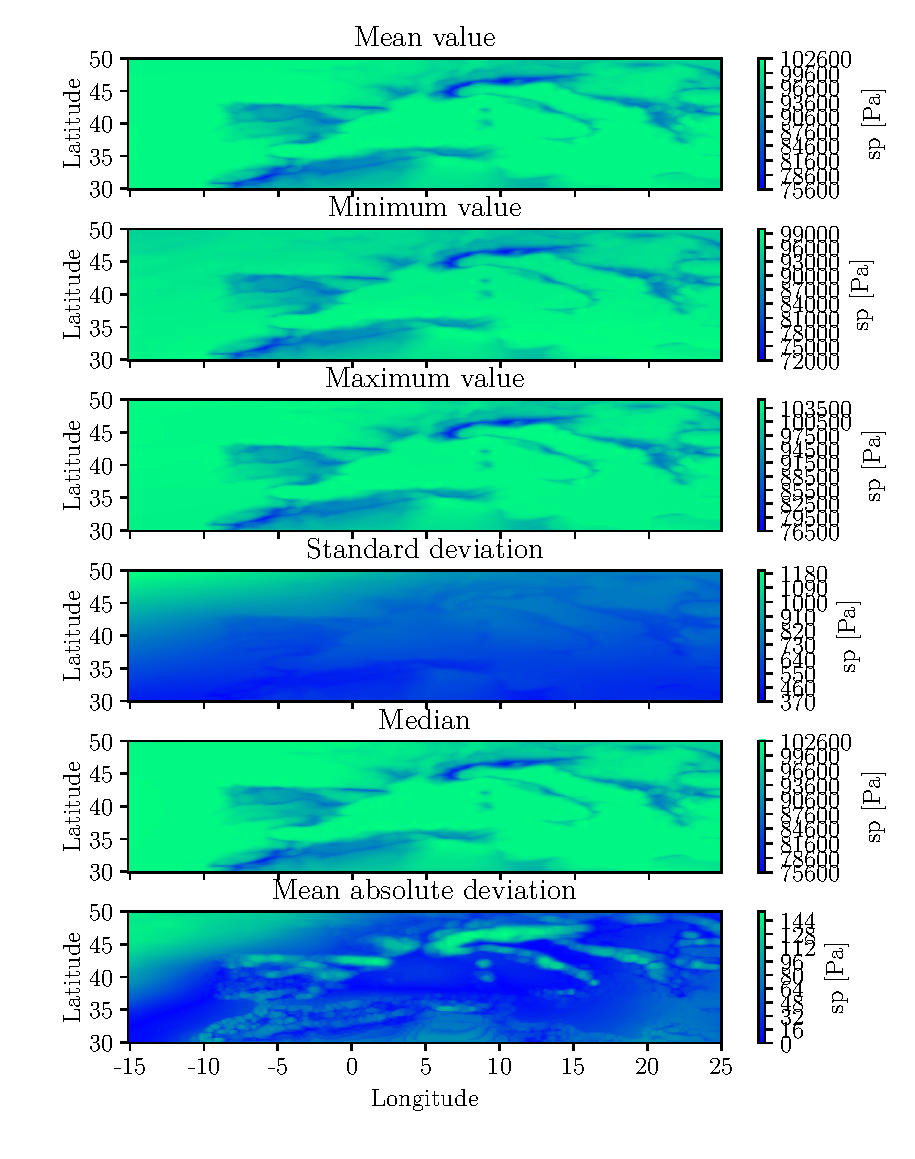
\includegraphics{python_figs/all_stat_variable_sp.pdf}
    \caption{Contour plot showing the local (pixel) statistics for surface pressure.}
    \label{fig:all_stats_sp}
\end{figure}

%% RELATIVE HUMIDITY 
\begin{figure}[ht]
    \centering
    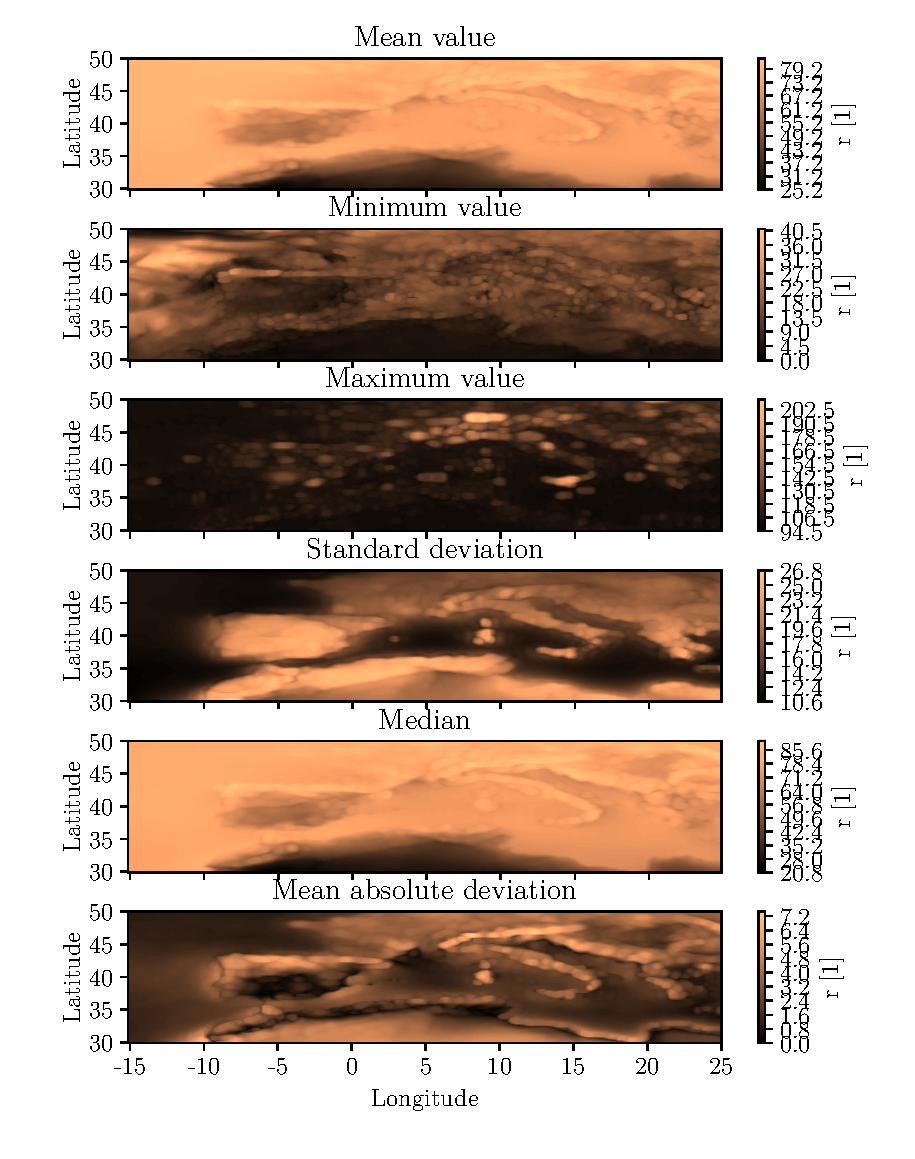
\includegraphics{python_figs/all_stat_variable_r.pdf}
    \caption{Contour plot showing the local (pixel) statistics for relative humidity.}
    \label{fig:all_stats_r}
\end{figure}


%% SPECIFIC HUMIDITY 
\begin{figure}[ht]
    \centering
    \includegraphics{python_figs/all_stat_variable_q.pdf}
    \caption{Contour plot showing the local (pixel) statistics for spesific humidity.}
    \label{fig:all_stats_q}
\end{figure}


\begin{figure}
    \centering
    \includegraphics{python_figs/signal_artefact.png}
    \caption{Occurence of artefact, keep in mind that is not made any effort to distinguish this from when the entire area has cloud cover, this could be done by the ratio of artefact signal to land or something else. }
    \label{fig:signal_artefact}
\end{figure}

%%%%%% CONTOUR PLOTS SHOWING 
%\subsection{Alternative 2 - sortert basert på statestikk }
%%%% STD
\begin{figure}[ht]
    \centering
    \includegraphics{python_figs/contourplot_all_variables_std.pdf}
    \caption{Contour plot showing the local (pixel) standard deviation of all variables.}
    \label{fig:contour_std_all_vars}
\end{figure}

%%%% MIN
\begin{figure}[ht]
    \centering
    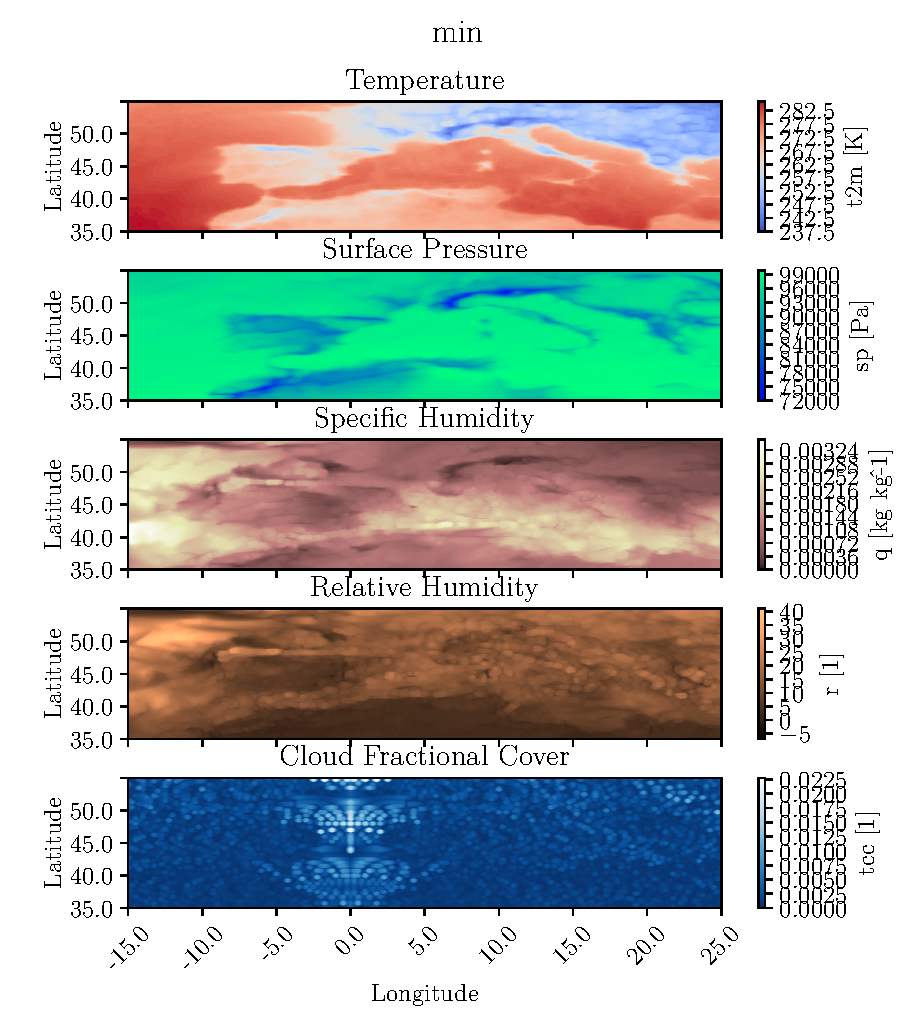
\includegraphics{python_figs/contourplot_all_variables_min.pdf}
    \caption{Contour plot showing the local (pixel) minimum of all variables.}
    \label{fig:contour_min_all_vars}
\end{figure}


%%%% MAX
\begin{figure}[ht]
    \centering
    \includegraphics{python_figs/contourplot_all_variables_max.pdf}
    \caption{Contour plot showing the local (pixel) max of all variables.}
    \label{fig:contour_max_all_vars}
\end{figure}


%%%% MAD
\begin{figure}[ht]
    \centering
    \includegraphics{python_figs/contourplot_all_variables_mad.pdf}
    \caption{NOT generated yet! Contour plot showing the local (pixel) mad of all variables.}
    \label{fig:contour_mad_all_vars}
\end{figure}


%%%% MEAN
\begin{figure}[ht]
    \centering
    \includegraphics{python_figs/contourplot_all_variables_mean.pdf}
    \caption{Contour plot showing the local (pixel) mean of all variables.}
    \label{fig:contour_mean_all_vars}
\end{figure}


%%%% MEDIAN
\begin{figure}[ht]
    \centering
    \includegraphics{python_figs/contourplot_all_variables_median.pdf}
    \caption{Contour plot showing the local (pixel) median of all variables.}
    \label{fig:contour_mean_all_vars}
\end{figure}


%%%%%%%%%%%%%%%%%%%%%%%%%%%5 seasonal statistics 

\cleardoublepage
\begin{figure}[ht]
    \centering
    \includegraphics{python_figs/contourplot_all_variables_median.pdf}
    \caption{Contour plot showing the local (pixel) median of all variables.}
    \label{fig:contour_mean_all_vars}
\end{figure}

\chapter{Performance of other models}


%%%% TARGET PREDICITON HORIZONTAL
\begin{figure}[ht]
    \centering
    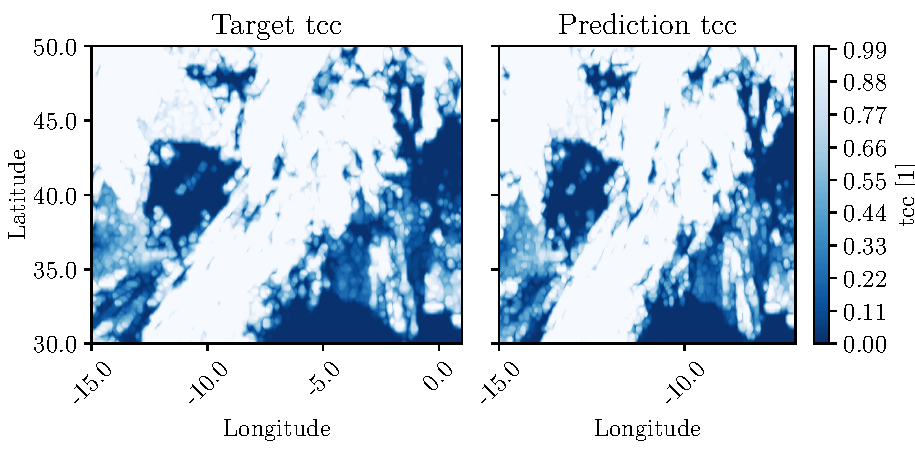
\includegraphics{python_figs/target_prediction_plot_horizonal.pdf}
    \caption{Comparison target and predicted cloud fractional cover.}
    \label{fig:target_predict_horizontal}
\end{figure}

%%%% TARGET PREDICITON HORIZONTAL
\begin{figure}[ht]
    \centering
    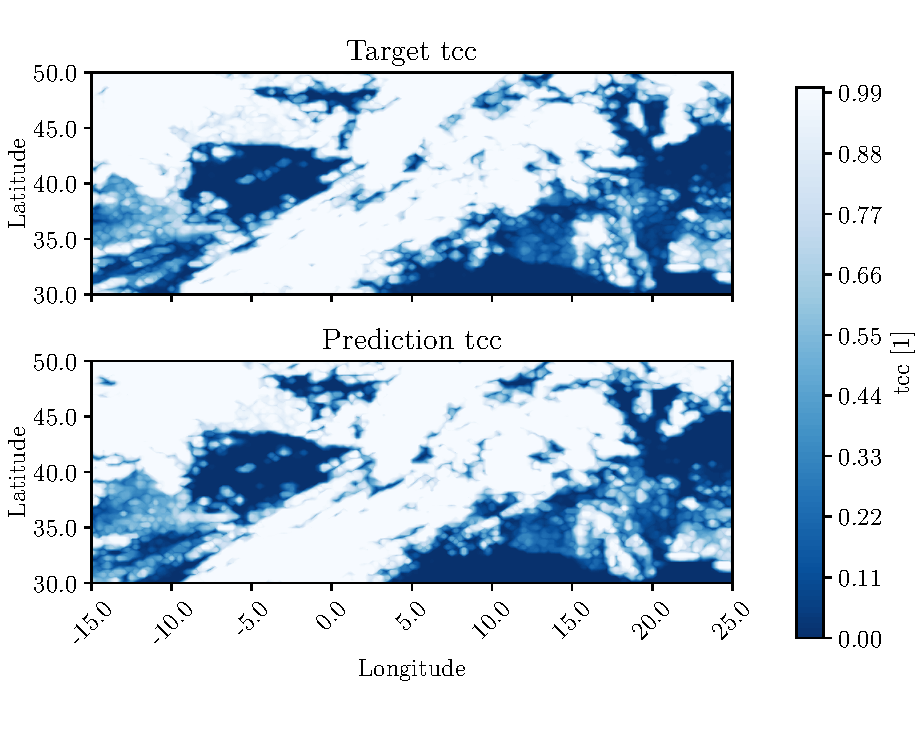
\includegraphics{python_figs/target_prediction_plot_vertical.pdf}
    \caption{Comparison target and predicted vertical cloud fractional cover.}
    \label{fig:target_predict_vertical}
\end{figure}

%%%% TARGET PREDICITON ERA5
\begin{figure}[ht]
    \centering
    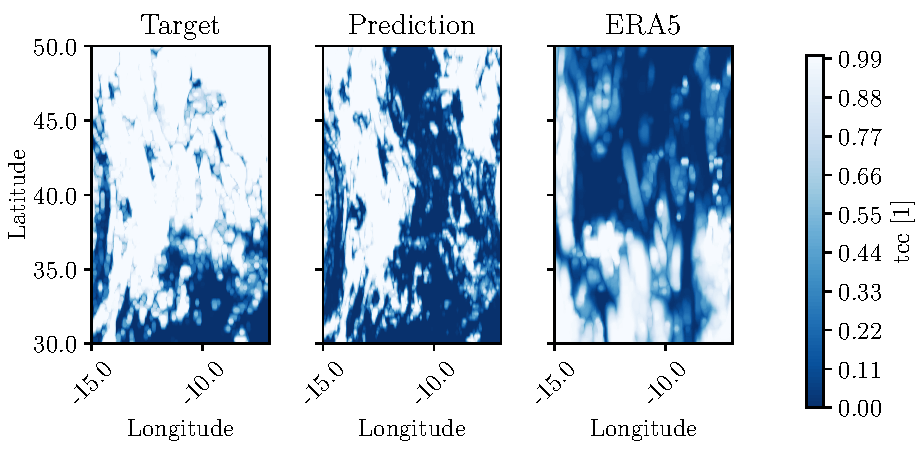
\includegraphics{python_figs/target_prediction_era5_plot_horizonal.pdf}
    \caption{Comparison target, predicted and era5 horizontal cloud fractional cover.}
    \label{fig:target_predict_era5_vertical}
\end{figure}

%%%%%%%%%% Traditional AR model
%\begin{figure}[ht]
%    \centering
%    \includegraphics{python_figs/test_traditional_ar_r2.png}
%    \caption{Trained model traditional ar of order 2. Ove land it seems ok, over ocean and montain area seems difficult.}
%    \label{fig:traditional_ar_model_order_1}
%\end{figure}

%%%%%%%%%% Dummy model performance plot
%\begin{figure}[ht]
%    \centering
%    \includegraphics{python_figs/dummy_model_performace_plot.pdf}
%    \caption{Dummy performance plot.}
%    \label{fig:dummy_performace_plot}
%\end{figure}

%%%%%%%%%% Dummy model performance plot - CROSSVALIDATION
%\begin{figure}[ht]
%    \centering
%    \includegraphics{python_figs/dummy_model_performace_cross_validation_plot.pdf}
%    \caption{Dummy performance plot - Crossvalidation edition.}
%    \label{fig:dummy_performace_plot_crossvalidation}
%\end{figure}

\cleardoublepage


\chapter{Time lapse cloud cover}

\begin{figure}[ht]
    \centering
    \includegraphics[scale=0.7]{python_figs/timelapse_cloud_cover_24hrs_from_2010-07-01.png}
    \caption{Time lapse photo, trying to detect the signal you would get from cloud cover within 24 hours.}
    \label{fig:time_lapse}
\end{figure}



\chapter{Study seasonal signals as temporal sequences - first week of every month in 2012}
%\addcontentsline{toc}{chapter}{Appendix D: Study 2012}

\begin{figure}[ht]
    \centering
    \includegraphics{python_figs/spatially_averaged_one_week_from_2012-01-01.png}
    \caption{Signal January 2012.}
    \label{fig:jan12}
\end{figure}

\begin{figure}[ht]
    \centering
    \includegraphics{python_figs/spatially_averaged_one_week_from_2012-02-01.png}
    \caption{Signal February 2012.}
    \label{fig:feb12}
\end{figure}

\begin{figure}[ht]
    \centering
    \includegraphics{python_figs/spatially_averaged_one_week_from_2012-01-01.png}
    \caption{Signal March 2012.}
    \label{fig:jan12}
\end{figure}
\begin{figure}[ht]
    \centering
    \includegraphics{python_figs/spatially_averaged_one_week_from_2012-03-01.png}
    \caption{Signal January 2012.}
    \label{fig:jan12}
\end{figure}
\begin{figure}[ht]
    \centering
    \includegraphics{python_figs/spatially_averaged_one_week_from_2012-04-01.png}
    \caption{Signal April 2012.}
    \label{fig:april12}
\end{figure}



\begin{figure}[ht]
    \centering
    \includegraphics{python_figs/spatially_averaged_one_week_from_2012-05-01.png}
    \caption{Signal May 2012.}
    \label{fig:may12}
\end{figure}


\begin{figure}[ht]
    \centering
    \includegraphics{python_figs/spatially_averaged_one_week_from_2012-06-01.png}
    \caption{Signal June 2012.}
    \label{fig:jun12}
\end{figure}

\begin{figure}[ht]
    \centering
    \includegraphics{python_figs/spatially_averaged_one_week_from_2012-07-01.png}
    \caption{Signal July 2012.}
    \label{fig:jul12}
\end{figure}

\begin{figure}[ht]
    \centering
    \includegraphics{python_figs/spatially_averaged_one_week_from_2012-08-01.png}
    \caption{Signal August 2012.}
    \label{fig:jan12}
\end{figure}

\begin{figure}[ht]
    \centering
    \includegraphics{python_figs/spatially_averaged_one_week_from_2012-09-01.png}
    \caption{Signal September 2012.}
    \label{fig:sep12}
\end{figure}


\begin{figure}[ht]
    \centering
    \includegraphics{python_figs/spatially_averaged_one_week_from_2012-10-01.png}
    \caption{Signal October 2012.}
    \label{fig:oct12}
\end{figure}


\begin{figure}[ht]
    \centering
    \includegraphics{python_figs/spatially_averaged_one_week_from_2012-11-01.png}
    \caption{Signal November 2012.}
    \label{fig:nov12}
\end{figure}

\begin{figure}[ht]
    \centering
    \includegraphics{python_figs/spatially_averaged_one_week_from_2012-12-01.png}
    \caption{Signal December 2012.}
    \label{fig:dec12}
\end{figure}

\chapter{Seasonal effects}
%\addcontentsline{toc}{chapter}{Seasonal effects}
This section has more plots. 
\begin{figure}[ht]
    \centering
    \includegraphics{python_figs/seasonal_mean_all_variables.png}
    \caption{Seasonal mean}
    \label{fig:seasonal_mean}
\end{figure}


\begin{figure}[ht]
    \centering
    \includegraphics{python_figs/seperate_colorbar_seasonal_std_all_variables.png}
    \caption{Need a colorbar for each plot to study the standard deviation, since the model output has so low std. Seasonal standarddeviation. }
    \label{fig:seasonal_std}
\end{figure}

\cleardoublepage

\addcontentsline{toc}{chapter}{Bibliography}
\printbibliography
\cleardoublepage

\end{document}
